% From https://github.com/UWIT-IAM/UWThesis

\documentclass [11pt, proquest] {uwthesis}[2015/03/03]


% fix for pandoc 1.14
\providecommand{\tightlist}{%
  \setlength{\itemsep}{0pt}\setlength{\parskip}{0pt}}

\newtheorem{theorem}{Jibberish}

\hyphenation{mar-gin-al-ia}

\usepackage[stamp]{draftwatermark}
% % Use the following to make modification
\SetWatermarkText{DRAFT}
\SetWatermarkLightness{0.95}

\usepackage[nointegrals]{wasysym} %% for the per mil symbol
\usepackage{textcomp}             %% for copyright symbol
\usepackage{lscape}               %% to allow to rotate pages to landscape
\usepackage{tabularx}             %% to adjust table column width
\usepackage{booktabs}             %% for more attractive tables
\usepackage{longtable}

% suppress bottom page numbers on first page of each chapter
% because they overlap with text
\usepackage{etoolbox}
\patchcmd{\chapter}{plain}{empty}{}{}




% Double spacing, if you want it.
% \def\dsp{\def\baselinestretch{2.0}\large\normalsize}
% \dsp

% If the Grad. Division insists that the first paragraph of a section
% be indented (like the others), then include this line:
% \usepackage{indentfirst}

%%%%%%%%%%%%%%%%%%
% If you want to use "sections" to partition your thesis
% un-comment the following:
% \counterwithout{section}{chapter}
% \setsecnumdepth{subsubsection}
% \def\sectionmark#1{\markboth{#1}{#1}}
% \def\subsectionmark#1{\markboth{#1}{#1}}
% \renewcommand{\thesection}{\arabic{section}}
% \renewcommand{\thesubsection}{\thesection.\arabic{subsection}}
% \makeatletter
% \let\l@subsection\l@section
% \let\l@section\l@chapter
% \makeatother
%
% \renewcommand{\thetable}{\arabic{table}}
% \renewcommand{\thefigure}{\arabic{figure}}
%%%%%%%%%%%%%%%%%%

%% This is my infobox class
\usepackage{graphicx}
\usepackage{xcolor}
\usepackage{mdframed}
\definecolor{infoblue}{RGB}{238, 247, 250}

% Helpful demo of using mdframded
% https://latex.org/forum/viewtopic.php?p=80700&sid=e0de1d6e3f5658d0778166a187b2a7ec#p80700
\newenvironment{infobox}
   {
    \begin{spacing}{0.95}\small
     % \raggedright
     % \textbf{Example: }%
   }{
   \end{spacing}
   }
\surroundwithmdframed[
   hidealllines=true,
   backgroundcolor=infoblue
]{infobox}

% Trick to have markdown inside of LaTeX environments get rendered
% # https://github.com/jgm/pandoc/issues/3145#issuecomment-302787889
\let\Begin\begin
\let\End\end



%% Stuff from https://github.com/suchow/Dissertate

% The following line would print the thesis in a postscript font

% \usepackage{natbib}
% \def\bibpreamble{\protect\addcontentsline{toc}{chapter}{Bibliography}}
% \bibliography{references}

\setcounter{tocdepth}{1}  % Print the chapter and sections to the toc

\usepackage{biblatex}

\prelimpages

%% from thesisdown
% To pass between YAML and LaTeX the dollar signs are added by CII
\Title{Development of word recognition in preschoolers}
\Author{Tristan Mahr}
\Year{2018}
\School{University of Wisconsin--Madison}
\Program{Communication Sciences and Disorders}
\Chair{Name of my committee chair}
\Signature{}
\Signature{}

% commands and environments needed by pandoc snippets
% extracted from the output of `pandoc -s`
%% Make R markdown code chunks work
\usepackage{array}
\usepackage{amssymb,amsmath}
\usepackage{ifxetex,ifluatex}
\ifxetex
  \usepackage{fontspec,xltxtra,xunicode}
  \defaultfontfeatures{Mapping=tex-text,Scale=MatchLowercase}
\else
  \ifluatex
    \usepackage{fontspec}
    \defaultfontfeatures{Mapping=tex-text,Scale=MatchLowercase}
  \else
    \usepackage[utf8]{inputenc}
  \fi
\fi
\usepackage{color}
\usepackage{fancyvrb}
\DefineShortVerb[commandchars=\\\{\}]{\|}
\DefineVerbatimEnvironment{Highlighting}{Verbatim}{commandchars=\\\{\}}
% Add ',fontsize=\small' for more characters per line
\newenvironment{Shaded}{}{}
\newcommand{\KeywordTok}[1]{\textcolor[rgb]{0.00,0.44,0.13}{\textbf{{#1}}}}
\newcommand{\DataTypeTok}[1]{\textcolor[rgb]{0.56,0.13,0.00}{{#1}}}
\newcommand{\DecValTok}[1]{\textcolor[rgb]{0.25,0.63,0.44}{{#1}}}
\newcommand{\BaseNTok}[1]{\textcolor[rgb]{0.25,0.63,0.44}{{#1}}}
\newcommand{\FloatTok}[1]{\textcolor[rgb]{0.25,0.63,0.44}{{#1}}}
\newcommand{\CharTok}[1]{\textcolor[rgb]{0.25,0.44,0.63}{{#1}}}
\newcommand{\StringTok}[1]{\textcolor[rgb]{0.25,0.44,0.63}{{#1}}}
\newcommand{\CommentTok}[1]{\textcolor[rgb]{0.38,0.63,0.69}{\textit{{#1}}}}
\newcommand{\OtherTok}[1]{\textcolor[rgb]{0.00,0.44,0.13}{{#1}}}
\newcommand{\AlertTok}[1]{\textcolor[rgb]{1.00,0.00,0.00}{\textbf{{#1}}}}
\newcommand{\FunctionTok}[1]{\textcolor[rgb]{0.02,0.16,0.49}{{#1}}}
\newcommand{\RegionMarkerTok}[1]{{#1}}
\newcommand{\ErrorTok}[1]{\textcolor[rgb]{1.00,0.00,0.00}{\textbf{{#1}}}}
\newcommand{\NormalTok}[1]{{#1}}
\newcommand{\OperatorTok}[1]{\textcolor[rgb]{0.00,0.44,0.13}{\textbf{{#1}}}}
\newcommand{\BuiltInTok}[1]{\textcolor[rgb]{0.00,0.44,0.13}{\textbf{{#1}}}}
\newcommand{\ControlFlowTok}[1]{\textcolor[rgb]{0.00,0.44,0.13}{\textbf{{#1}}}}


\ifxetex
  \usepackage[setpagesize=false, % page size defined by xetex
              unicode=false, % unicode breaks when used with xetex
              xetex,
              colorlinks=true,
              linkcolor=blue]{hyperref}
\else
  \usepackage[unicode=true,
              colorlinks=true,
              linkcolor=blue]{hyperref}
\fi
\hypersetup{breaklinks=true, pdfborder={0 0 0}}
\setlength{\parindent}{0pt}
\setlength{\parskip}{6pt plus 2pt minus 1pt}
\setlength{\emergencystretch}{3em}  % prevent overfull lines
\setcounter{secnumdepth}{0}



\begin{document}
\copyrightpage

\titlepage

\setcounter{page}{-1}
\abstract{Here is my abstract}

\tableofcontents
\listoffigures
\listoftables

\acknowledgments{My acknowledgments}

\dedication{\begin{center}For Penny\end{center}}

\textpages

\frontmatter

\chapter*{Preface}\label{preface}
\addcontentsline{toc}{chapter}{Preface}

This book, when finished, will contain my dissertation research.
\begin{itemize}
\tightlist
\item
  Last compiled: 2018-04-13 10:19:24
\end{itemize}
\mainmatter

\part*{Prospectus}\label{part-prospectus}
\addcontentsline{toc}{part}{Prospectus}

\chapter{Prospectus Preamble}\label{prospectus-preamble}

\section*{About This Document}\label{about-this-document}
\addcontentsline{toc}{section}{About This Document}

This document outlines the research questions, data, and methods for my
dissertation. This proposal started out as a grant-writing project, so
it has some of the touchstones of NIH F31 grant (Specific Aims,
Significance, Approach), but these sections have been expanded
considerably.

Date of oral presentation of dissertation proposal: April 3, 2017.

\section*{Dissertation Committee Members}\label{committee-members}
\addcontentsline{toc}{section}{Dissertation Committee Members}
\begin{itemize}
\item
  Jan Edwards, primary mentor and chair, Department of Hearing and
  Speech Sciences, University of Maryland
\item
  Susan Ellis Weismer, advisor at UW-Madison, Department of
  Communication Sciences and Disorders
\item
  Margarita Kaushanskaya, Department of Communication Sciences and
  Disorders
\item
  Audra Sterling, Department of Communication Sciences and Disorders
\item
  David Kaplan, Department of Educational Psychology
\item
  Bob McMurray, Department of Psychological and Brain Sciences,
  University of Iowa
\end{itemize}
\section*{Planned Dissertation
Format}\label{planned-dissertation-format}
\addcontentsline{toc}{section}{Planned Dissertation Format}

Two thematically related manuscripts, one for each specific aim, to be
completed by Summer 2018.

\chapter{Specific Aims}\label{specific-aims}

Individual differences in language ability are apparent as soon as
children start talking, but it is difficult to identify children at risk
for language delay or disorder. Recent work suggests word recognition
efficiency---that is, how well children map incoming speech to
words---may help identify early differences in children's language
trajectories. Children learn spoken language by listening to caregivers,
so children who are faster at recognizing words have an advantage for
word learning. This view is borne out by some studies suggesting that
children who are faster at processing words show greater vocabulary
gains months later (e.g., Weisleder \& Fernald,
\protect\hyperlink{ref-Weisleder2013}{2013}).

We do not know, however, how word recognition itself develops over time
within a child. This is an important open question because word
recognition may provide a key mechanism for understanding how individual
differences emerge in word learning and persist into early language
development. Without a developmental account of word recognition, we
lack the context for understanding individual differences in lexical
processing. Thus, even the big-picture questions are unclear: Do early
differences persist over time so that faster processors remain
relatively fast later in childhood? Or, is such a question ill-posed
because the magnitude of the differences among children shrink with age?
I plan to address this gap in knowledge by analyzing three years of word
recognition data collected in recently completed longitudinal study of
180 children.

In particular, I will examine the development of \emph{familiar word
recognition}, \emph{lexical competition,} and \emph{fast referent
selection} (the ability to map novel words to novel objects in the
moment). Through these analyses, I will develop a fine-grained
description of how the dynamics of word recognition change year over
year, and I will study how differences in word recognition performance
relate to child-level measures (such as vocabulary and speech
perception). I will complement these empirical analyses with
computational cognitive models. With these models, I will simulate the
word recognition data from each year and study how the models need to
change to adapt to children's developing word recognition abilities.
These simulations can identify plausible psychological mechanisms that
underlie changes in word recognition behavior.

\section{Specific Aim 1 (Familiar Word Recognition and Lexical
Competition)}\label{specific-aim-1-familiar-word-recognition-and-lexical-competition}

\textbf{To characterize the development of familiar word recognition and
lexical competition, I will analyze data from a visual world paradigm
experiment, conducted at age 3, age 4, and age 5.}

In these eyetracking experiments, children were presented with four
images of familiar objects and heard a prompt to view one of the images.
The four images included a target word (e.g., \emph{bell}), a
semantically related word (\emph{drum}), a phonologically similar word
(\emph{bee}), and an unrelated word (\emph{swing}). I will use a series
of growth curve analyses to describe how children's familiar word
recognition develop year over year. Of interest is how individual
differences at Year 1 persist into Year 3. I will also analyze how
expressive vocabulary and lexical processing develop together over time.
Lastly, I will examine the children's looks to the distractors to study
the developmental course of lexical competition from similar sounding
and similar meaning words. Changes in sensitivity to competing words can
reveal how lexical competition emerges as a byproduct of learning new
words.

\section{Specific Aim 2 (Referent Selection and
Mispronunciations)}\label{specific-aim-2-referent-selection-and-mispronunciations}

\textbf{To characterize how fast referent selection develops
longitudinally, I will analyze data from a looking-while-listening
mispronunciation experiment, conducted at age 3, age 4, and age 5.}

In these eyetracking experiments (Law \& Edwards,
\protect\hyperlink{ref-MPPaper}{2015}; based on White \& Morgan,
\protect\hyperlink{ref-WhiteMorgan2008}{2008}), children saw an image of
a familiar object and an unfamiliar object, and they heard either a
correct production of the familiar object (e.g., \emph{soup}), a
one-feature mispronunciation of the familiar object (\emph{shoop}), or a
novel word unrelated to either image (\emph{cheem}). The correct
productions test familiar word recognition and the nonwords test fast
referent selection. The mispronunciations test a child's phonological
categories (whether the child permits, rejects, or equivocates about
mispronunciations).

I will use growth curve analyses to study how children's responses to
the three word types change over time. I will examine familiar word
recognition and fast referent selection to determine which feature of
lexical processing better predicts vocabulary growth. I plan to examine
dissociations or asymmetries in these forms of processing within
children as a way to empirically assess the claim that ``novel word
processing (referent selection) is not distinct from familiar word
recognition'' (McMurray, Horst, \& Samuelson,
\protect\hyperlink{ref-McMurray2012}{2012}). Finally, I will examine how
individual differences in vocabulary and speech perception predict
responses to mispronunciations and novel words.

\section{Summary}\label{summary}

This project investigates how word recognition develops during the
preschool years. There has been no research studying word recognition
longitudinally after age two. Findings will show how individual
differences in lexical processing change over time and can reveal how
low-level mechanisms underlying word recognition mature longitudinally
in children. These findings will have translational value by studying
processing abilities that subserve word learning and by assessing the
predictive relationships between early word recognition ability and
later language outcomes.

\chapter{Significance}\label{significance}

\section{Public Health Significance}\label{public-health-significance}

Vocabulary size in preschool is a robust predictor of later language
development, and early language skills predict early literacy skills at
school entry (P. L. Morgan, Farkas, Hillemeier, Hammer, \& Maczuga,
\protect\hyperlink{ref-Morgan2015}{2015}). By studying the mechanisms
that shape word learning, we can understand how individual differences
in language ability arise and identify strategies for closing language
gaps between children. Word recognition---the process of mapping
incoming speech sounds to known or novel words---has been shown to
predict later language outcomes. We do not know how this ability
develops over time, and we do not know when word recognition is most
predictive of future outcomes. This project will provide an integrated
account of how word recognition and its relationship with vocabulary
size change from age~3 to age~5.

\section{Scientific Significance}\label{scientific-significance}

\subsection{Lexical Processing
Dynamics}\label{lexical-processing-dynamics}

Mature listeners recognize words by continuously evaluating incoming
speech input for possible word matches through lexical competition. The
first part of a word activates multiple candidate words in parallel, and
these candidates compete so that the best-fitting word is recognized.
For example, the onset ``bee'' might activate the candidates \emph{bee},
\emph{beam}, \emph{beetle}, \emph{beak}, \emph{beaker},
\emph{beginning}, and so on, but an additional ``m'' would narrow the
candidates to just \emph{beam}. Semantic relationships also influence
lexical processing, and cascading phonological-semantic effects---e.g.,
where \emph{castle} activates the phonologically similar \emph{candy}
which in turn activates the semantically related \emph{sweet}---have
been demonstrated (Marslen-Wilson \& Zwitserlood,
\protect\hyperlink{ref-Marslen-Wilson1989}{1989}). Both low-level
phonetic cues and high-level grammatical, semantic and pragmatic
information can influence this process, but the \emph{continuous
processing of multiple competing candidates} is the essential dynamic
underlying word recognition (Magnuson, Mirman, \& Myers,
\protect\hyperlink{ref-Magnuson2013}{2013}).

What about young children who know considerably fewer words? Eyetracking
studies with toddlers have suggested a developmental continuity between
toddlers and adult listeners. Children recognize words incrementally
(Swingley, Pinto, \& Fernald,
\protect\hyperlink{ref-Swingley1999}{1999}), match truncated words to
their intended referents (Fernald, Swingley, \& Pinto,
\protect\hyperlink{ref-Fernald2001}{2001}), and use information from
neighboring words in a sentence to facilitate word recognition. This
information can be grammatical: Lew-Williams \& Fernald
(\protect\hyperlink{ref-Lew-Williams2007}{2007}) found that
Spanish-acquiring preschoolers can use grammatical gender on determiners
(\emph{el} or \emph{la}) to anticipate the word named in a two-object
word recognition task. The information can also be subcategorical
phonetic variation: We found that English-acquiring toddlers look
earlier to a named image when the coarticulatory formant cues on word
\emph{the} predict the noun of the sentence, compared to tokens with
neutral coarticulation (Tristan Mahr, McMillan, Saffran, Ellis Weismer,
\& Edwards, \protect\hyperlink{ref-Mahr2015}{2015}).

There is some evidence for lexical competition where children are
sensitive to phonological and semantic similarities among words. Ellis
Weismer, Haebig, Edwards, Saffran, \& Venker
(\protect\hyperlink{ref-EllisWeismer2016}{2016}) showed that toddlers
(14--29 months old) looked less reliably to a named image when the
onscreen competitor was a semantically related word or perceptually
similar image. In Law, Mahr, Schneeberg, \& Edwards
(\protect\hyperlink{ref-RWLPaper}{2016}), preschoolers (28--60 months
old) demonstrated sensitivity to semantic and phonological competitors
in a four-image eyetracking task. Huang \& Snedeker
(\protect\hyperlink{ref-Huang2011}{2011}) presented evidence of
cascading semantic-phonological activation in five-year-olds such that
for a target word like \emph{log}, children looked more to an indirect
phonological competitor like \emph{key} (competing through its
activation of \emph{lock}) than they looked to an unrelated image like
\emph{carrot}. In contrast to these studies which all demonstrate
interference from similar words, Mani \& Plunkett
(\protect\hyperlink{ref-Mani2010}{2010}) demonstrated cross-modal
phonological priming effects in 18-month-olds. In this study, a picture
of prime word (e.g., cat or teeth) was presented in silence; then two
images (e.g., cup and shoe) were presented, one of which was named
(\emph{cup}). Children on average looked more to the target word (like
\emph{cup}) when it was primed by an image of a phonological neighbor
(like \emph{cat}), and the children performed at chance when the prime
was not related to the named word. Mani, Durrant, \& Floccia
(\protect\hyperlink{ref-Mani2012}{2012}) found a similar result for
cascading phonological-semantic priming with 24-month-olds: Children
looked more to a target \emph{shoe} compared to a distractor \emph{door}
when primed by an image of \emph{clock}, assumed to activate \emph{sock}
which primed \emph{shoe}.

The above studies involved young children of different ages tested under
different procedures, sometimes in different dialects and languages.
Averaging these results together, so to speak, the studies suggest that
early word recognition demonstrates some hallmarks of adult behavior:
Continuous processing of words, integration of information from
different levels of representation, and the influence of similar,
unspoken words on recognition of a word. Nevertheless, we only have a
fragmented view of how familiar word recognition and lexical competition
develop within children.

One open question is how lexical competition develops within children.
For example, do phonological similar words exert more interference
during word recognition as children grow older? As a guiding hypothesis,
we can think of word learning as a gradual process where familiarity
with a word moves from shallow receptive knowledge to deeper expressive
knowledge. In adult listeners, words compete and inhibit one another, so
that a word is truly ``learned'' and integrated into the lexicon when it
can influence the processing of other words (a line of reasoning
reviewed by Kapnoula, Packard, Gupta, \& McMurray,
\protect\hyperlink{ref-Kapnoula2015}{2015}). Increasing sensitivity to
similar sounding words over time would reveal that children improve
their ability to consider multiple candidates in parallel. By studying
how sensitivity to similar-sounding and similar-meaning words develop
over time and within ever-growing vocabularies, this project can reveal
how children come to process words efficiently.

Another avenue for studying word recognition is to examine how listeners
respond to unfamiliar or novel stimuli. A productive line of research
has found that children are sensitive to mispronunciations during word
recognition (e.g., Swingley \& Aslin,
\protect\hyperlink{ref-Swingley2000}{2000},
\protect\hyperlink{ref-Swingley2002}{2002}). White \& Morgan
(\protect\hyperlink{ref-WhiteMorgan2008}{2008}) presented toddlers with
images of a familiar and novel object, and children heard a correct
production of the familiar object, mispronunciations of the familiar
object of varying severity, or an unrelated nonword. Toddlers looked
less to a familiar word when the first segment was mispronounced.
Moreover, they demonstrated graded sensitivity such that a 1-feature
mispronunciation yielded more looks to an image than a 2-feature
mispronunciation, and a 2-feature mispronunciation yielded more looks
than a 3-feature one. Finally, in the nonword condition, the children
looked more to the novel object than the familiar one, demonstrating
\emph{fast referent selection} as they associated novel words to novel
objects in the moment. A similar pattern of effects was observed in the
mispronunciation study by Law \& Edwards
(\protect\hyperlink{ref-MPPaper}{2015}) with preschoolers mapping real
words to familiar objects, nonwords to novel objects, and equivocating
about mispronunciations of familiar words.

As with lexical competition, it is unclear how children's responses to
mispronunciations and novel words change over time or how individual
differences among children change over time. For example, do children
become more forgiving of mispronunciations as they mature and learn more
words? We might expect so, as children become more experienced at
listening to noisy, degraded, or misspoken speech.

Another open question involves the development of fast referent
selection. At face value, we might expect a child's ability to associate
new words with unfamiliar objects to be more direct measure of
word-learning capacity than a child's ability to process known words.
Under this assumption, we would expect individual differences in fast
referent selection to be highly correlated with vocabulary growth. But
McMurray et al. (\protect\hyperlink{ref-McMurray2012}{2012}) propose
that the same basic process is at play in both recognition of familiar
words and fast association of nonwords. In experiments, the observed
behaviors are the same: Children hear a word and direct their attention
to an appropriate referent. This project can tackle these questions by
describing how mispronunciations are processed as children grow older
and by examining whether familiar word recognition and fast referent
selection dissociate and which one is a better predictor of vocabulary
growth.

\subsection{Individual Differences in Word
Recognition}\label{individual-differences-in-word-recognition}

We have a rough understanding of the development of word recognition,
and these gaps in knowledge matter because young children differ in
their word recognition abilities. These differences are usually measured
using \emph{accuracy} (a probability of recognizing to a word) or
\emph{efficiency} (a reaction time or some measure of how quickly
accuracy changes over time). These differences are consequential too, as
word recognition differences correlate with other language measures
concurrently, retrospectively, and prospectively.

The best predictor of lexical processing efficiency is concurrent
vocabulary size: Children who know more words look more quickly and
reliably to a named word (e.g., Law \& Edwards,
\protect\hyperlink{ref-MPPaper}{2015}).

This fact deserves a brief reflection: Suppose the information
processing mechanism behind word recognition were just a naïve table
search. Then this finding is somewhat puzzling: Children with larger
lexicons have to find a needle in a larger haystack---yet this apparent
liability is an advantage. That is why the search analogy is naïve. One
explanation follows from the earlier described idea about graded word
learning: Children become better at recognizing words as they learn more
words because they extract regularities and discover similarities among
words and develop more efficient lexical representations---the haystack
develops regularity and becomes easier to search.

Although it is a robust predictor of word recognition, vocabulary size
is nonspecific. For lexical processing dynamics, vocabulary size can be
considered an indicator for the organization and efficiency of a child's
lexicon, but it also correlates with other (meaningful) differences.
Vocabulary is related to differences in speech perception (Cristia,
Seidl, Junge, Soderstrom, \& Hagoort,
\protect\hyperlink{ref-Cristia2014_Review}{2014}) and environmental
factors like language input (e.g., Hart \& Risley,
\protect\hyperlink{ref-HartRisley}{1995}; Hoff,
\protect\hyperlink{ref-Hoff2003}{2003}). For instance, measures of
speech perception at 6--8 months predict vocabulary size at 24 months
(Kuhl et al., \protect\hyperlink{ref-Kuhl2008}{2008}; e.g., Tsao, Liu,
\& Kuhl, \protect\hyperlink{ref-Tsao2004}{2004}), so processing predicts
future vocabulary predicts concurrent processing.

A related complication is the apparent predictive validity of word
recognition measures. Marchman \& Fernald
(\protect\hyperlink{ref-MarchmanFernald2008}{2008}) found that
vocabulary size and lexical processing efficiency at age~2 jointly
predicted working memory scores and expressive language scores at age~8.
This result would suggest domain-general processing advantages influence
word learning. Fernald \& Marchman
(\protect\hyperlink{ref-Fernald2012}{2012}) also found that late talkers
who looked more quickly to a named word at 18 months showed larger gains
in vocabulary by 30 months compared to late-talkers who looked more
slowly at 18 months. Weisleder \& Fernald
(\protect\hyperlink{ref-Weisleder2013}{2013}) found that lexical
processing and language input at 19~months predict vocabulary size at 25
months and that lexical processing mediated the effect of language
input.

Word recognition efficiency and vocabulary size are interconnected
measures with concurrent and predictive associations. This project can
clarify this relationship by examining the co-development of word
recognition, vocabulary size, and speech perception. In particular, I
will ask how individual differences in word recognition change over time
alongside differences in vocabulary. I can also which features of word
recognition (fast referent selection, lexical competition, etc.) are
most predictive of vocabulary outcomes at age~5. The additional measures
of speech perception can also help clarify the specific effects of
vocabulary size on word recognition.

\subsection{Summary}\label{summary-1}

This project studies word recognition in children over three years, so
it will provide the first longitudinal study of word recognition in
preschoolers. Children in this cohort cover a range of vocabulary scores
at Time~1, and this variability allows one to investigate individual
differences in vocabulary and word recognition over time and assess the
predictive value of these measures. Furthermore, this project studies
word recognition in two experimental tasks that can tap into different
aspects of word recognition. Specifically, a four-image experiment with
semantic and phonological foils allows me to study how lexical
competition develops, and a two-image experiment with nonwords and
mispronunciations enables me to study how fast referent selection
develops over time as well. I will use mixed effects modeling to study
not just gross measures of accuracy or interference from distractors,
but the time course and lexical dynamics of word recognition using
growth curve analyses.

\chapter{Research Hypotheses}\label{research-hypotheses}

In this section, I outline the main hypotheses I plan to study for each
specific aim. This section is intended to preregister the main analyses
for this project, so I can cleanly separate confirmatory and exploratory
results.

\section{Specific Aim 1 (Familiar Word Recognition and Lexical
Competition)}\label{specific-aim-1-familiar-word-recognition-and-lexical-competition-1}
\begin{itemize}
\item
  Children's accuracy and efficiency of recognizing words will improve
  each year.
\item
  There are stable individual differences in lexical processing of
  familiar words such that children who are relatively fast at age~3
  remain relatively fast at age~4 and age~5.
\item
  However, the magnitude of these individual differences diminishes over
  time, as children converge on a mature level of performance for this
  paradigm.
\item
  As a consequence, individual differences in word recognition at age~3,
  for example, will be more discriminating and predictive of age~5
  language outcomes than differences at age~4.
\item
  Children will become more sensitive to lexical competitors as they
  age, based on the hypothesis that children discover similarities among
  words as a consequence of learning more and more words.
\item
  Children will differ in their sensitivity to lexical competitors, and
  these individual differences will correlate with other child-level
  measures.
\end{itemize}
\section{Specific Aim 2 (Referent Selection and
Mispronunciations)}\label{specific-aim-2-referent-selection-and-mispronunciations-1}
\begin{itemize}
\item
  Children's accuracy and efficiency of recognizing real words and
  fast-associating nonwords will improve each year.
\item
  Performance in real word recognition and fast association of nonwords
  will be highly correlated, based on the hypothesis that the same
  process (referent selection) operates in both situations.
\item
  Under the alternative hypothesis, real word recognition and fast
  referent selection reflect different skills with different
  developmental trajectories. Thus, if there is any dissociation between
  recognition of real words and nonwords, it will be observed in younger
  children.
\item
  Although these two measures will be correlated, I predict performance
  in the nonword condition will be a better predict of future vocabulary
  growth than performance in the real word condition. This hypothesis is
  based on the idea that fast referent selection is a more relevant
  skill for learning new words than recognition of known words.
\item
  For the mispronunciations, I predict children with larger vocabularies
  (that is, older children) will be more likely to tolerate a
  mispronunciation as a production of familiar word compared to children
  with smaller vocabularies.
\item
  Mispronunciations that feature later-mastered sounds (e.g.,
  \emph{rice}/\emph{wice}) will be more likely to be associated to novel
  objects than earlier-mastered sounds (\emph{duck}/\emph{guck}).
\end{itemize}
\part*{Aim 1: Familiar Word Recognition and Lexical
Competition}\label{part-aim1}
\addcontentsline{toc}{part}{Aim 1: Familiar Word Recognition
and Lexical Competition}

\chapter{Method}\label{aim1-method}

\section{Participants}\label{participants}

The participants were 28--39 months-old at Age~3, 39--52 at Age~4, and
51--65 at Age~5. Approximately, 180 children participated at Age~3, 170
at Age~4, and 160 at Age~5. Of these children, approximately 20 were
identified by their parents as late talkers. Prospective families were
interviewed over telephone before participating in the study. Children
were not scheduled for testing if a parent reported language problems,
vision problems, developmental delays, or an individualized education
program for the child. Recruitment and data collection occurred at two
Learning to Talk lab sites---one at the University of Wisconsin--Madison
and the other at the University of Minnesota.

Table \ref{tab:participant-info} summarizes the cohort of children in
each year of testing. The numbers and summary statistics here are
general, describing children who participated at each year, but whose
data may have been excluded from the analyses. Some potential reasons
for exclusion include: excessive missing data during eyetracking,
experiment or technology error, developmental concerns not identified
until later in study, or a failed hearing screening. Final sample sizes
will depend on the measures needed for an analysis and the results from
data screening checks. I disclose all measurements and data exclusions
following guidelines by the Center for Open Science (Nosek et al.,
\protect\hyperlink{ref-OSF_Statement}{2014}).
\begin{longtable}[]{@{}llll@{}}
\caption{\label{tab:participant-info} Participant characteristics. Education
levels: \emph{Low}: less than high school, or high school;
\emph{Middle}: trade school, technical or associates degree, some
college, or college degree; and \emph{High}: graduate
degree.}\tabularnewline
\toprule
& Year 1 (Age 3) & Year 2 (Age 4) & Year 3 (Age 5)\tabularnewline
\midrule
\endfirsthead
\toprule
& Year 1 (Age 3) & Year 2 (Age 4) & Year 3 (Age 5)\tabularnewline
\midrule
\endhead
N & 184 & 175 & 160\tabularnewline
Boys, Girls & 94, 90 & 89, 86 & 82, 78\tabularnewline
Maternal education: Low, Middle, High & 15, 98, 71 & 12, 92, 71 & 6, 90,
64\tabularnewline
Dialect: MAE, AAE & 171, 13 & 163, 12 & 153, 7\tabularnewline
Parent-identified late talkers & 20 & 19 & 16\tabularnewline
Age (months): Mean (SD) {[}Range{]} & 33 (3) {[}28--39{]} & 45 (4)
{[}39--52{]} & 57 (4) {[}51--66{]}\tabularnewline
EVT-2 standard score: Mean (SD) & 115 (18) & 118 (16) & 118
(14)\tabularnewline
PPVT-4 standard score: Mean (SD) & 113 (17) & 120 (16) &
---\tabularnewline
GFTA-2 standard score: Mean (SD) & 92 (13) & --- & 91
(13)\tabularnewline
\bottomrule
\end{longtable}
\section{Procedure}\label{procedure}

This experiment used a version of the Visual World Paradigm for word
recognition experiments (Law et al.,
\protect\hyperlink{ref-RWLPaper}{2016}). In eyetracking studies with
toddlers, two familiar images are usually presented: a target and a
distractor. This experiment is a four-image eyetracking task that was
designed to provide a more demanding word recognition task for
preschoolers. In this procedure, four familiar images are presented
onscreen followed by a prompt to view one of the images (e.g.,
\emph{find the bell!}). The four images include the target word (e.g.,
\emph{bell}), a semantically related word (\emph{drum}), a
phonologically similar word (\emph{bee}), and an unrelated word
(\emph{swing}). Figure~\ref{fig:sample-vw-screen} shows an example of a
trial's items. This procedure measures a child's real-time comprehension
of words by capturing how the child's gaze location changes over time in
response to speech.




\begin{figure}
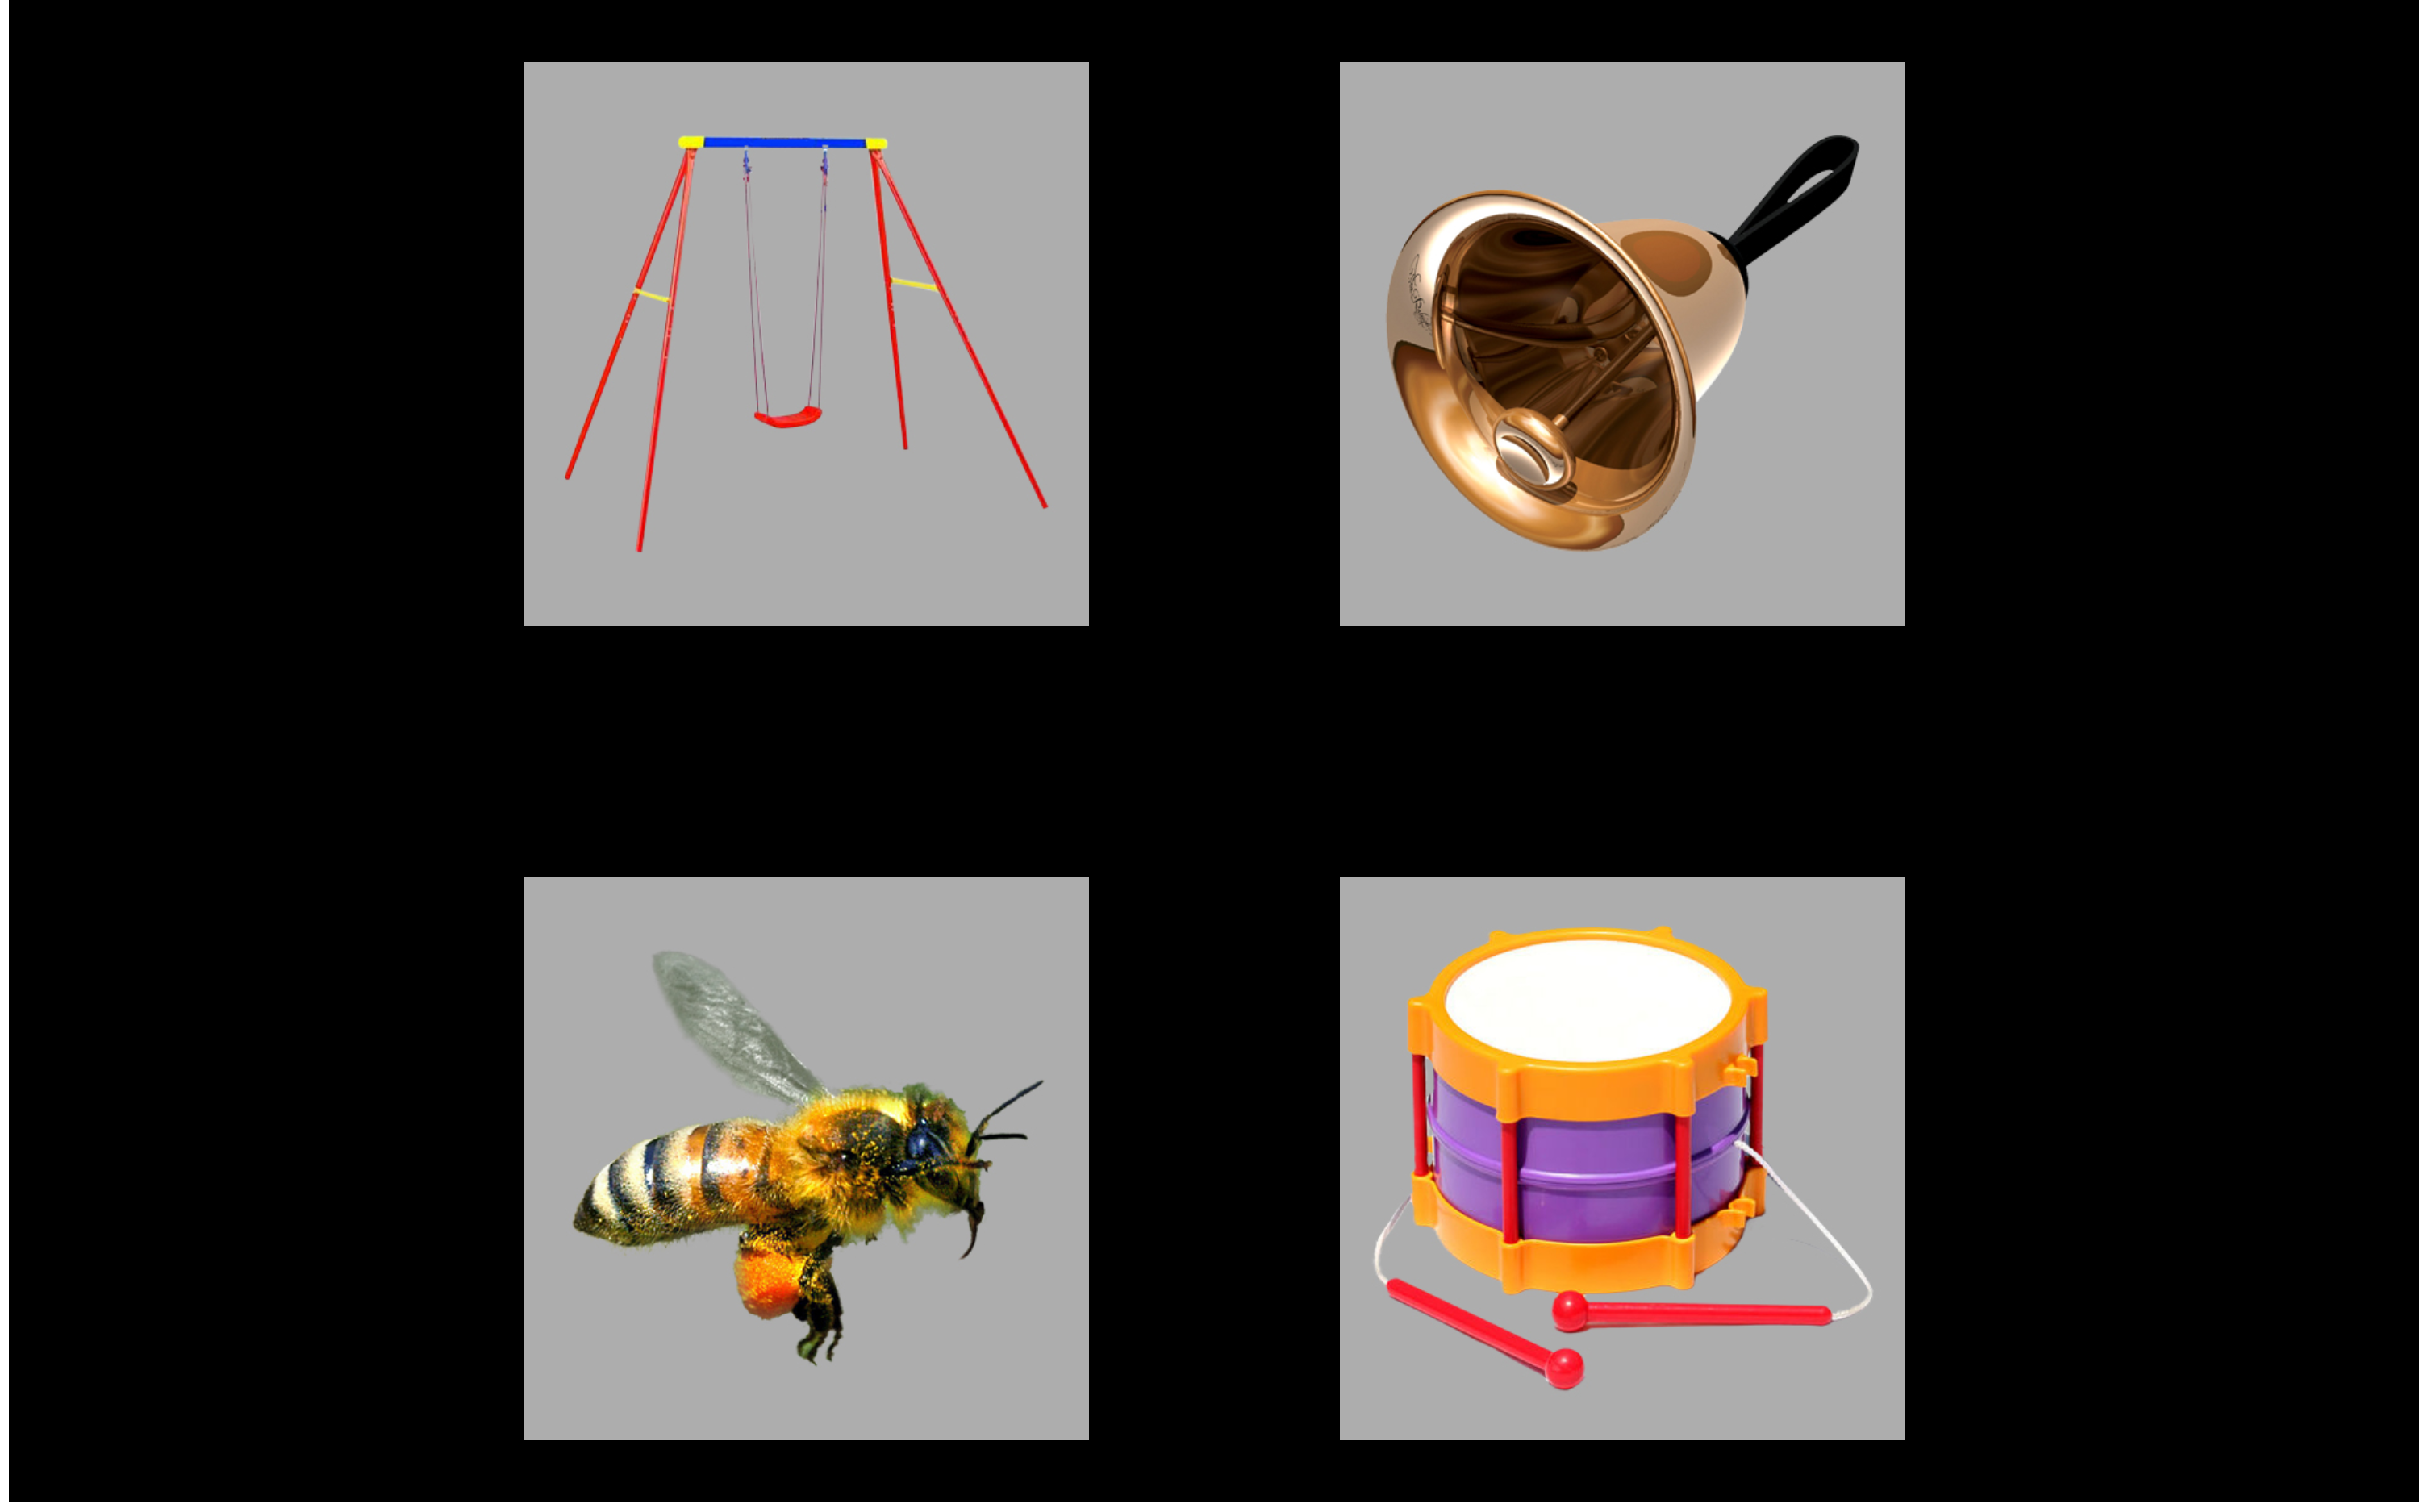
\includegraphics[width=1\linewidth]{./misc/rwl-screens/TimePoint1/actual/Block2_17_swing2_bell2_bee2_drum2_UpperRightImage_bell} \caption{Example display for the target \emph{bell}
with the semantic foil \emph{drum}, the phonological foil \emph{bee},
and the unrelated \emph{swing}.}\label{fig:sample-vw-screen}
\end{figure}
\section{Experiment Administration}\label{experiment-administration}

Children participating in the study were tested over two lab visits (on
different dates). The first portion of each visit involved ``watching
movies''---that is, performing two blocks of eyetracking experiments. A
play break or hearing screening occurred between the two eyetracking
blocks, depending on the visit.

Each eyetracking experiment was administered as a block of trials (24
for this experiment and 38 for a two-image task---see Chapter~X).
Children received two different blocks of each experiment. The blocks
for an experiment differed in trial ordering and other features.
Experiment order and block selection were counterbalanced over children
and visits. For example, a child might have received Exp.~1 Block~A and
Exp.~2 Block~B on Visit~1 and next received Exp.~2 Block~A and Exp.~1
Block~B on Visit~2. The purpose of this presentation was to control
possible ordering effects where a particular experiment or block
benefited from consistently occurring first or second.

Experiments were administered using E-Prime~2.0 and a Tobii T60XL
eyetracker which recorded gaze location at a rate of 60~Hz. The
experiments were conducted by two examiners, one ``behind the scenes''
who controlled the computer running the experiment and another
``onstage'' who guided the child through the experiment. At the
beginning of each block, the child was positioned so the child's eyes
were approximately 60~cm from the screen. The examiners calibrated the
eyetracker to the child's eyes using a five-point calibration procedure
(center of screen and centers of four screen quadrants). The examiners
repeated this calibration procedure if one of the five calibration
points for one of the eyes did not calibrate successfully. During the
experiment, the behind-the-scenes examiner monitored the child's
distance from the screen and whether the eyetracker was capturing the
child's gaze. The onstage examiner coached the child to stay fixated on
the screen and repositioned the child as needed to ensure the child's
eyes were being tracked. Every six or seven trials in a block of an
experiment, the experiment briefly paused with a reinforcing animation
or activity. During these breaks, the onstage examiner could reposition
the child if necessary before resuming the experiment.

We used a gaze-contingent stimulus presentation. First, the images
appeared in silence on screen for 2~s as a familiarization period. The
experiment then checked whether the child's gaze was being recorded. If
the experiment could continuously track the child's gaze for 300~ms, the
child's gaze was verified and the trial continued. If the experiment
could not verify the gaze after 10~s, the trial continued. This
procedure guaranteed that for most trials, the child was looking to the
display before presenting the carrier phrase and that the experiment was
ready to record the child's response to the carrier. During Year~1
(age~3) and Year~2 (age~4), an attention-getter (e.g., \emph{check it
out}!) played 1~s following the end of the target noun. These
reinforcers were dropped in Year~3 (age~5) to streamline the experiment
for older listeners.

\section{Stimuli}\label{stimuli}

The four images on each trial consisted of a target noun, a phonological
foil, a semantic foil, and an unrelated word. The phonological
competitors shared a syllable onset (e.g., \emph{flag}--\emph{fly},
\emph{bell}--\emph{bee}), shared an initial consonant
(\emph{bread}--\emph{bear}, \emph{swing}--\emph{spoon}), had a similar
phonetically similar consonant onset (\emph{kite}--\emph{gift}), or
shared a syllable rime (\emph{van}--\emph{pan}). The semantic
competitors included words from the same category (e.g.,
\emph{shirt}--\emph{dress}, \emph{horse}--\emph{bear}), words that were
perceptually similar (\emph{sword}--\emph{pen},
\emph{flag}--\emph{kite}), and words with less obvious relationships
(\emph{van}--\emph{horse}, \emph{swan}-\emph{bee}). A complete list of
the items used in the experiment in
\protect\hyperlink{vw-experiment-items}{Appendix
\ref{vw-experiment-items}}.

The stimuli were recorded in both Mainstream American English (MAE) and
African American English (AAE), so that the experiment could accommodate
the child's home dialect. Prior to the lab visit, we made a preliminary
guess about the child's home dialect, based on the recruitment channel,
address, among other factors. If we expected the dialect to be AAE, then
the lab visit was led by an examiner who natively spoke AAE and could
fluently dialect-shift between AAE and MAE. At the beginning of the lab
visit, the examiner listened to the interactions between the child and
caregiver in order to confirm the child's home dialect. Prompts to view
the target image of a trial (e.g., \emph{find the girl}) used the
carrier phrases ``find the'' and ``see the''. These carriers were
recording in the frame ``find/see the egg'' and cross-spliced with the
target nouns to minimize coarticulatory cues on the determiner ``the''.
The stimuli were re-recorded after the first year of the study with the
same speakers so that the average duration of the two dialect versions
were more similar.

The images used in the experiment consisted of color photographs on gray
backgrounds. These images were piloted with 30 children from two
preschool classrooms to ensure that children consistently used the same
label for familiar objects. The two preschool classrooms differed in
their students' SES demographics: One classroom (13 piloting students)
was part of a university research center which predominantly serves
higher-SES families, and the other classroom (17 piloting students) was
part of Head Start center which predominantly serves lower-SES families.
The images were tested by presenting four images (a target, a
phonological foil, a semantic foil and an unrelated word) and having the
student point to the named image. The pictures had to be recognized by
at least 80\%~of students in each classroom.

\section{Data screening}\label{data-screening}

To process the eyetracking data, I first mapped gaze \emph{x}-\emph{y}
coordinates onto the onscreen images. We next performed
\emph{deblinking}. I interpolated short runs of missing gaze data (up to
150~ms) if the same image was fixated before and after the missing data
run. Put differently, I classified a window of missing data as a blink
if the window was brief and the gaze remained on the same image before
and after the blink. I interpolated missing data from blinks using the
fixated image.

After mapping the gaze coordinates onto the onscreen images, I performed
data screening. I considered the time window from~0 to~2000~ms after
target noun onset. I identified a trial as \emph{unreliable} if at least
50\%~of the looks were missing during the time window. I excluded an
entire block of trials if it had fewer than 12 reliable trials.

Table~\ref{tab:screening-counts} shows the numbers of participants and
trials at each year before and after data screening. There were more
children in the second year than the first due to a timing error in the
initial version of this experiment, leading to the exclusion of 27
participants from the first year.
\begin{table}

\caption{\label{tab:screening-counts}Eyetracking data before and after data screening. For convenience, the number of exclusions are included as Raw - Screened.}
\centering
\begin{tabular}[t]{llrrr}
\toprule
Dataset & Study & N Children & N Blocks & N Trials\\
\midrule
Raw & Age 3 & 178 & 332 & 7967\\
 & Age 4 & 180 & 347 & 8327\\
 & Age 5 & 163 & 322 & 7724\\
Screened & Age 3 & 163 & 291 & 5951\\
 & Age 4 & 165 & 305 & 6421\\
\addlinespace
 & Age 5 & 156 & 295 & 6483\\
Raw \&minus; Screened & Age 3 & 15 & 41 & 2016\\
 & Age 4 & 15 & 42 & 1906\\
 & Age 5 & 7 & 27 & 1241\\
\bottomrule
\end{tabular}
\end{table}
\section{Model preparation}\label{model-preparation}

To prepare the data for modeling, I downsampled the data into 50-ms
(3-frame) bins, reducing the eyetracker's effective sampling rate to
20~Hz. Eye movements have durations on the order of~100 or 200~ms, so
capturing data every 16.67~ms oversamples eye movements and can
introduce high-frequency noise into the signal. Binning together data
from neighboring frames can smooth out this noise. I modeled the looks
from~250 to~1500~ms. Lastly, I aggregated looks by child, study and
time, and created orthogonal polynomials to use as time features for the
model.

Figure~\ref{fig:aim1-spaghetti} depicts the dataset following these data
screening and preparation steps. The lines start around .25 which is
chance performance on four-alternative forced choice task. The lines
rise as the word unfolds and peak and plateau around 1400~ms.





\begin{figure}
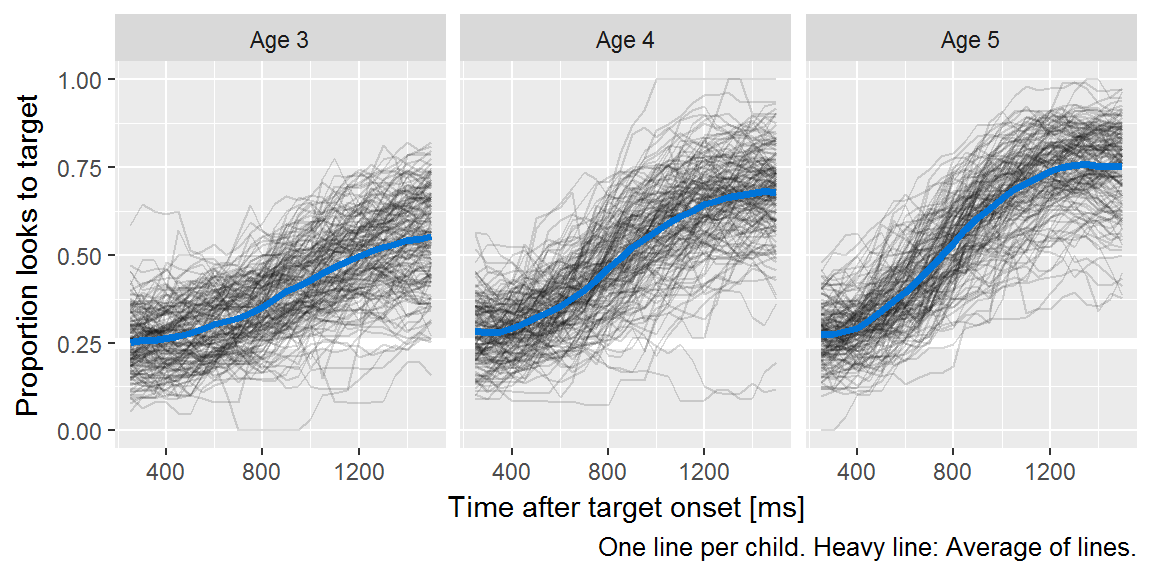
\includegraphics[width=1\linewidth]{12-aim1-methods_files/figure-latex/aim1-spaghetti-1} \caption{Empirical word recognition growth curves from each
year of the study. Each line represents an individual child's proportion
of looks to the target image over time. The heavy lines are the averages
of the lines for each year.}\label{fig:aim1-spaghetti}
\end{figure}
\chapter{Analysis of familiar word
recognition}\label{analysis-of-familiar-word-recognition}

\section{Growth curve analysis}\label{growth-curve-analysis}

Looks to the familiar image were analyzed using Bayesian mixed effects
logistic regression. I used \emph{logistic} regression because the
outcome measurement is a probability (the log-odds of looking to the
target image versus a distractor). I used \emph{mixed-effects} models to
estimate a separate growth curve for each child (to measure individual
differences in word recognition) but also treat each child's individual
growth curve as a draw from a distribution of related curves. I used
\emph{Bayesian} techniques to study a generative model of the data.
Instead of reporting and describing a single, best-fitting model of some
data, Bayesian methods consider an entire distribution of plausible
models that are consistent with the data and any prior information we
have about the models. By using this approach, one can explicitly
quantify uncertainty about statistical effects and draw inferences using
estimates of uncertainty (instead of using statistical
significance---which is not a straightforward matter for mixed-effects
models).\footnote{It is tempting to further justify this approach by
  comparing Bayesian versus classical/frequentist statistics, but my
  goals in using this method are simple: To estimate statistical effects
  and quantify uncertainty about those effects. This pragmatic brand of
  Bayesian statistics is illustrated in texts by Gelman \& Hill
  (\protect\hyperlink{ref-GelmanHill}{2007}) and McElreath
  (\protect\hyperlink{ref-RethinkingBook}{2016}).}

The eyetracking growth curves were fit using an orthogonal cubic
polynomial function of time (a now-conventional approach; see Mirman,
\protect\hyperlink{ref-Mirman2014}{2014}). Put differently, I modeled
the probability of looking to the target during an eyetracking task as:

\[
\text{log-odds}(\textit{looking}\,) = 
  \beta_0 + 
  \beta_1\text{Time}^1 + 
  \beta_2\text{Time}^2 + 
  \beta_3\text{Time}^3
\]

That the time terms are \emph{orthogonal} means that \(\text{Time}^1\),
\(\text{Time}^2\) and \(\text{Time}^3\) are transformed so that they are
uncorrelated. Under this formulation, the parameters \(\beta_0\) and
\(\beta_1\) have a direct interpretation in terms of lexical processing
performance. The intercept, \(\beta_0\), measures the area under the
growth curve---or the probability of fixating on the target word
averaged over the whole window. We can think of \(\beta_0\) as a measure
of \emph{word recognition reliability}. The linear time parameter,
\(\beta_1\), estimates the steepness of the growth curve---or how the
probability of fixating changes from frame to frame. We can think of
\(\beta_1\) as a measure of \emph{processing efficiency}, because growth
curves with stronger linear features exhibit steeper frame-by-frame
increases in looking probability.\footnote{The polynomial other terms
  are less important---or rather, they have do not map as neatly onto
  behavioral descriptions as the accuracy and efficiency parameters. The
  primary purpose of quadratic and cubic terms is to ensure that the
  estimated growth curve adequately fits the data. In this kind of data,
  there is a steady baseline at chance probability before the child
  hears the word, followed a window of increasing probability of
  fixating on the target as the child recognizes the word, followed by a
  period of plateauing and then diminishing looks to target. The cubic
  polynomial allows the growth curve to be fit with two inflection
  points: the point when the looks to target start to increase from
  baseline and the point when the looks to target stops increasing.}

To study how word recognition changes over time, I modeled how the
growth curves change over developmental time. This amounted to studying
how the growth curve parameters changes year over year. I included
dummy-coded indicators for Age~3, Age~4, and Age~5 and allowed these
indicators interact with the growth curve parameters. These
year-by-growth-curve terms captured how the shape of the growth curves
changed each year. The model also included random effects to represent
child-by-year effects.

\subsection{Growth curve features as measures of word recognition
performance}\label{growth-curve-features-as-measures-of-word-recognition-performance}

As mentioned above, two of the model's growth curve features have
straightforward interpretations in terms of lexical processing
performance: The model's intercept parameter corresponds to the average
proportion or probability of looking to the named image over the trial
window, and the linear time parameter corresponds to slope of the growth
curve or lexical processing efficiency. I also was interested in
\emph{peak} proportion of looks to the target. I derived this value by
computing the growth curves from the model and taking the median of the
five highest points on the curve. Figure \ref{fig:curve-features} shows
three simulated growth curves and how each of these growth curve
features relate to word recognition performance.




\begin{verbatim}
#> Warning: package 'bindrcpp' was built under R version 3.4.4
\end{verbatim}
\begin{figure}
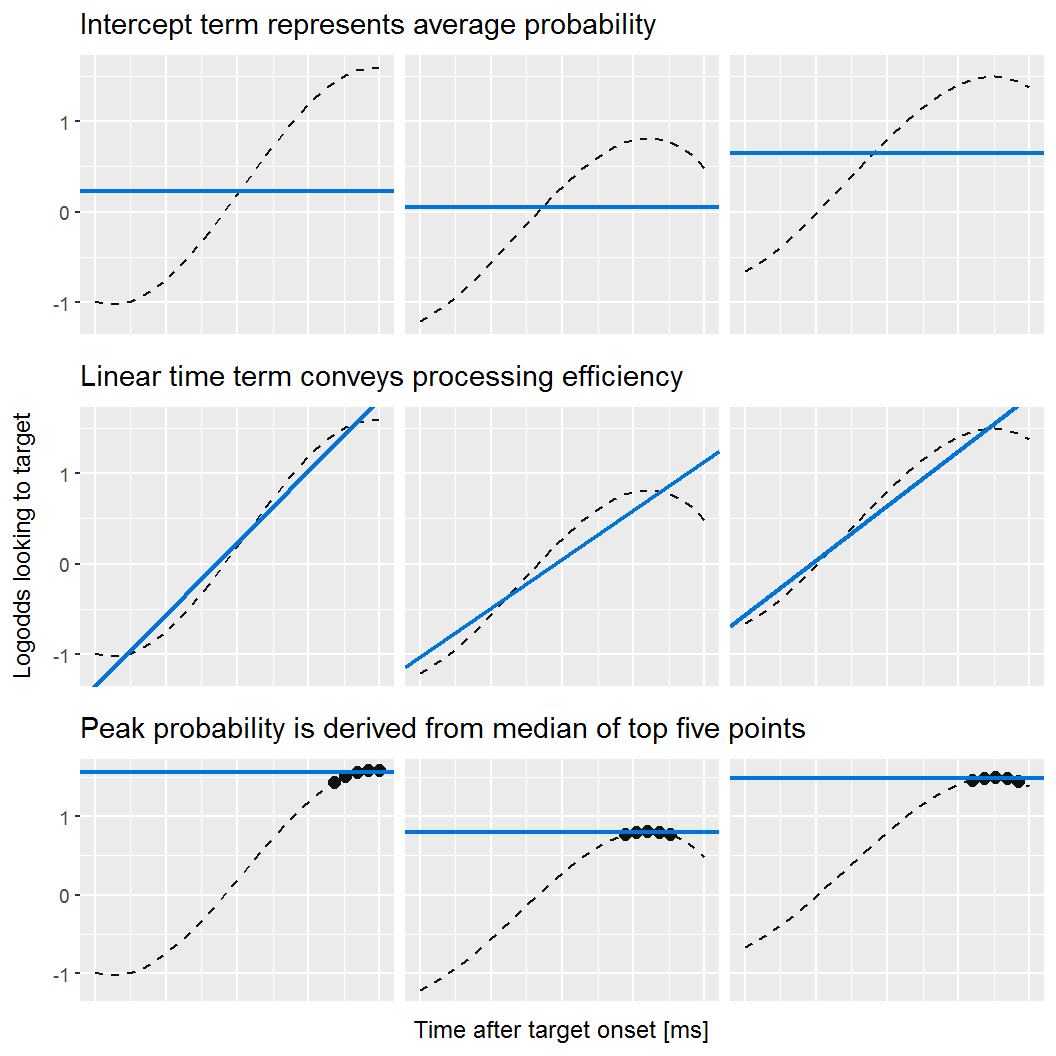
\includegraphics[width=0.8\linewidth]{14-aim1-familiar-word-recognition_files/figure-latex/curve-features-1} \caption{Illustration of the three growth curve features and
how they describe lexical processing performance. The three curves used
are simulations of new participants at Age~4.}\label{fig:curve-features}
\end{figure}
\section{Year over year changes in word recognition
performance}\label{year-over-year-changes-in-word-recognition-performance}

The mixed-effects model estimated a population-average growth curve
(``fixed'' effects) and how individual children deviated from average
(``random'' effects). Figure~\ref{fig:average-growth-curves} shows 200
posterior samples of the average growth curves for each study. On
average, the growth curves become steeper and achieve higher looking
probabilities with each year of the study.





\begin{figure}
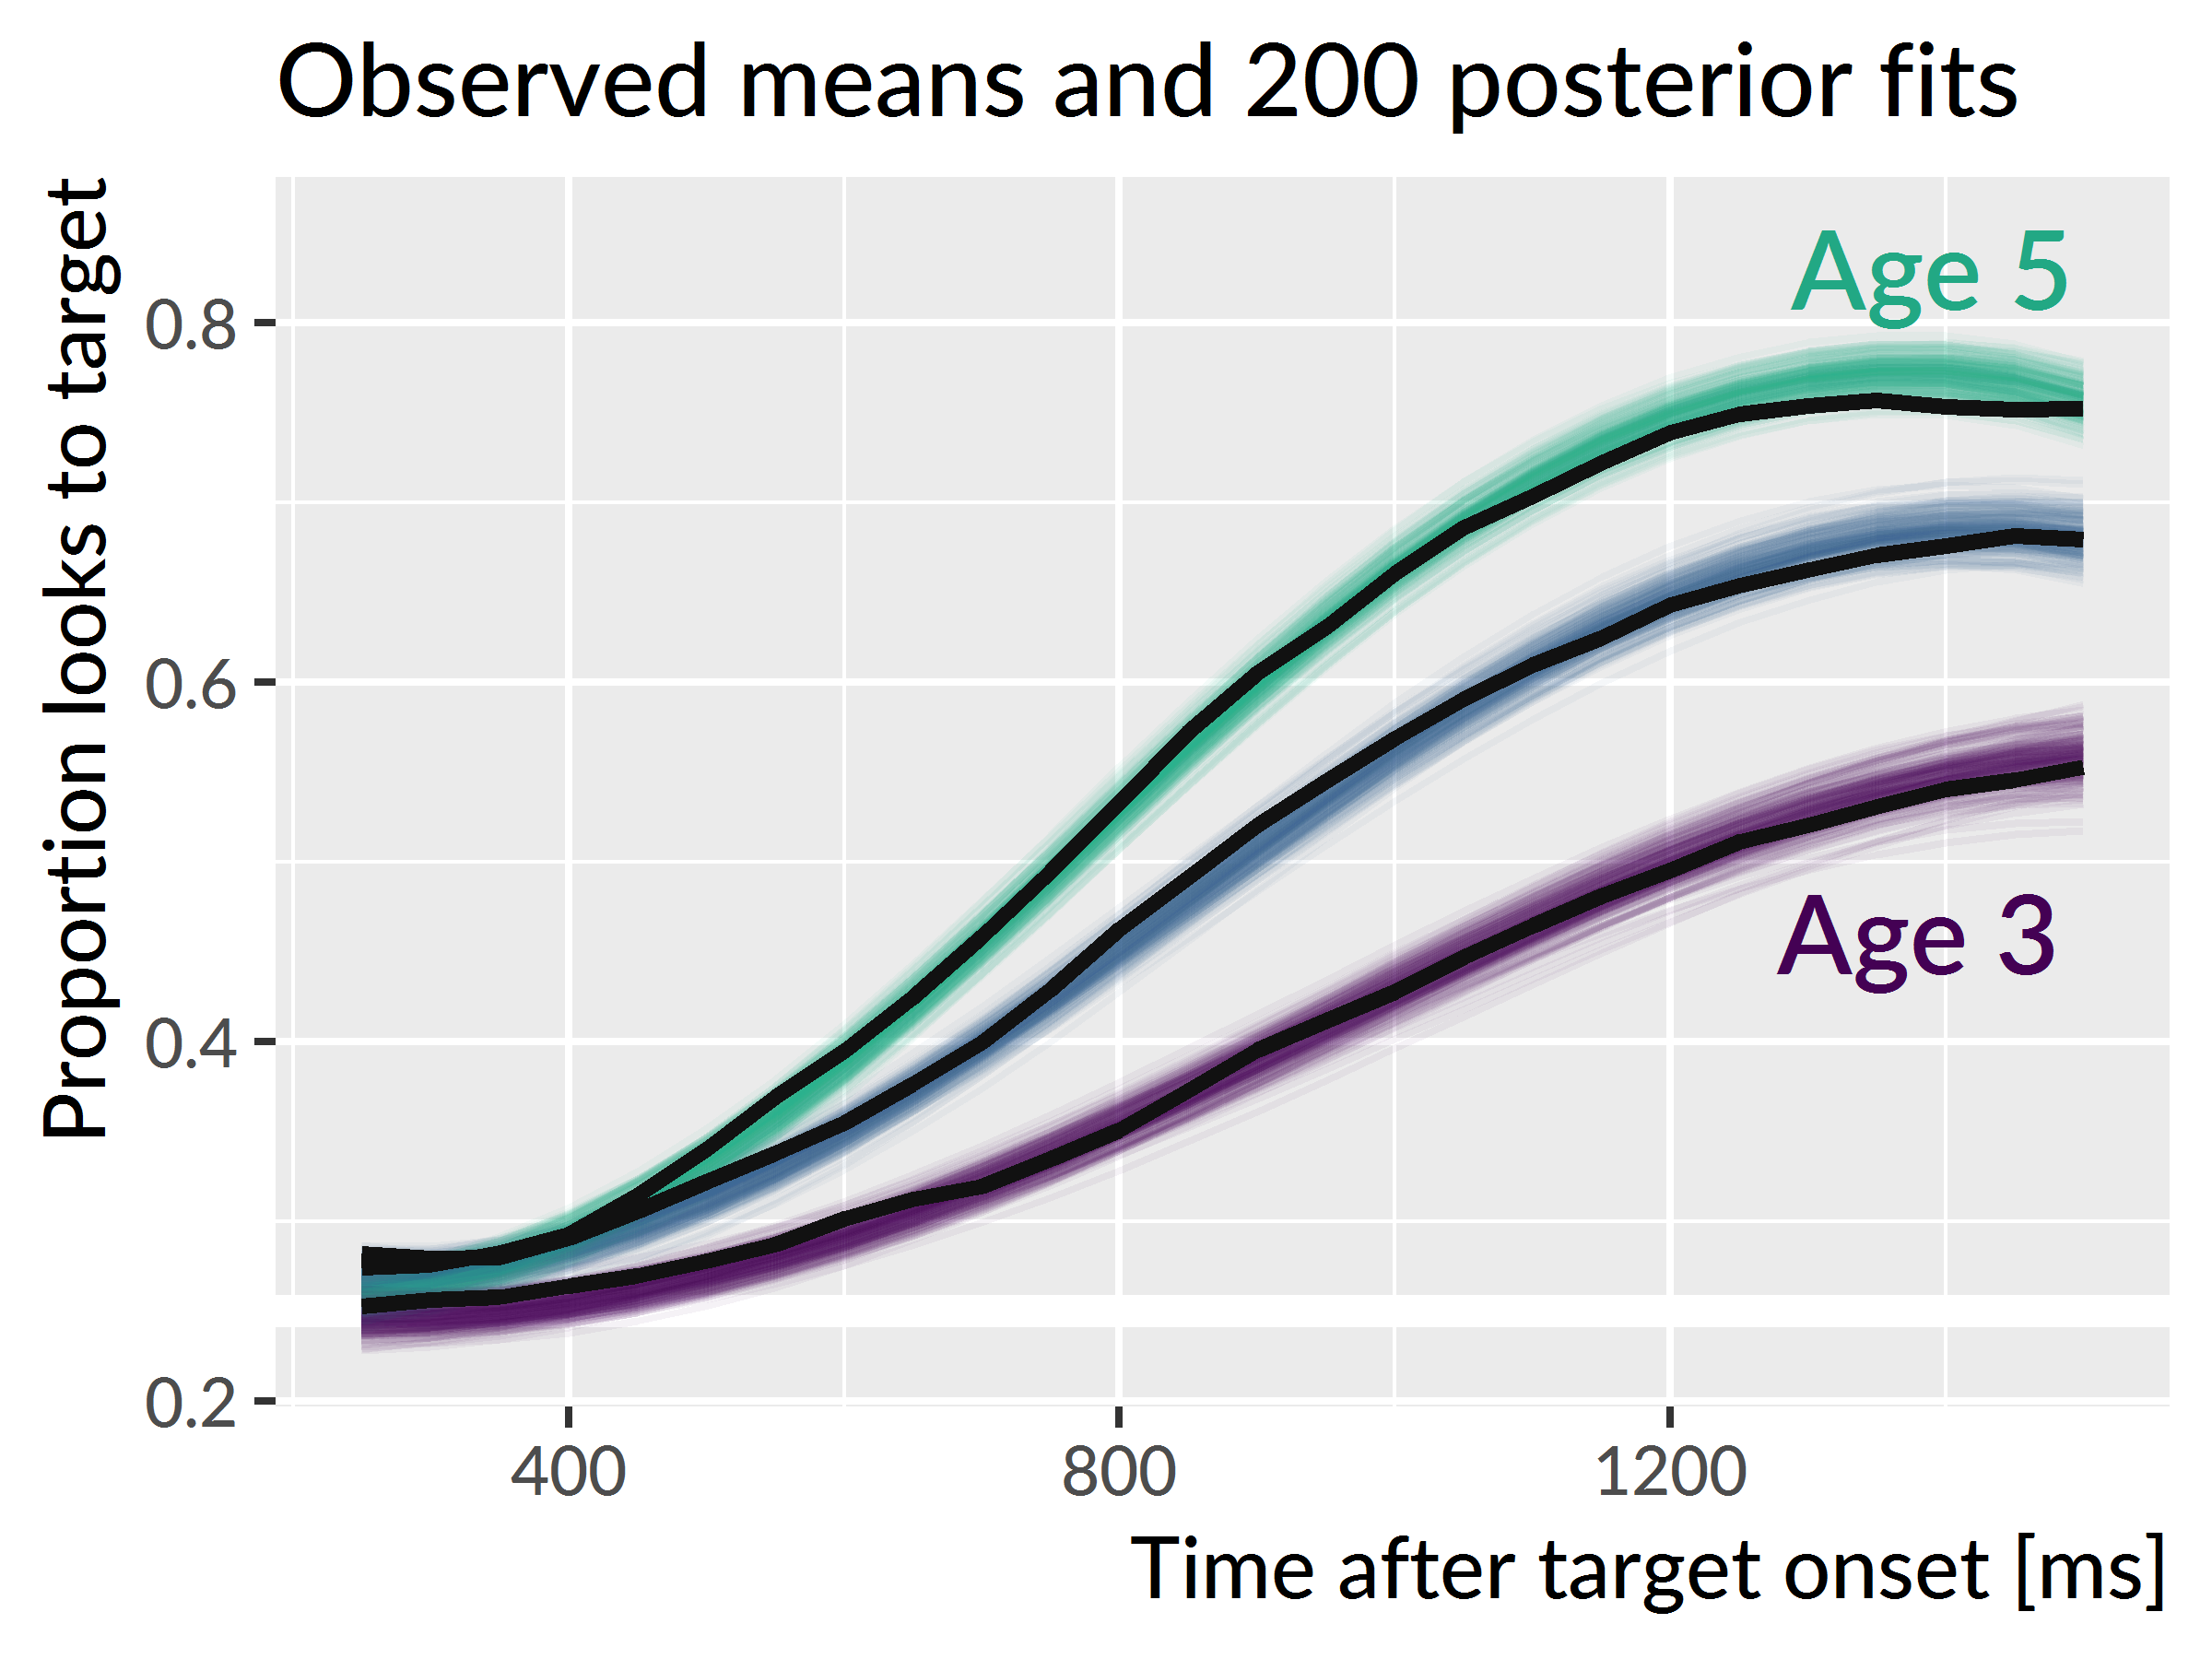
\includegraphics[width=0.5\linewidth]{14-aim1-familiar-word-recognition_files/figure-latex/average-growth-curves-1} \caption{The model estimated an average word
recognition growth for each study, and the colored lines represent 200
posterior samples of these growth curves. The thick dark lines represent
the observed average growth curve in each study.}\label{fig:average-growth-curves}
\end{figure}
Figure~\ref{fig:effects2} depicts uncertainty intervals with the model's
average effects of each timepoint on the growth curve features. The
intercept and linear time effects increased each year, confirming that
children become more reliable and faster at recognizing words as they
grow older. The peak accuracy also increased each year. For each effect,
the change from age~3 to age~4 is approximately the same as the change
from age~4 to age~5, as visible in Figure~\ref{fig:pairwise-effects}.




\begin{figure}
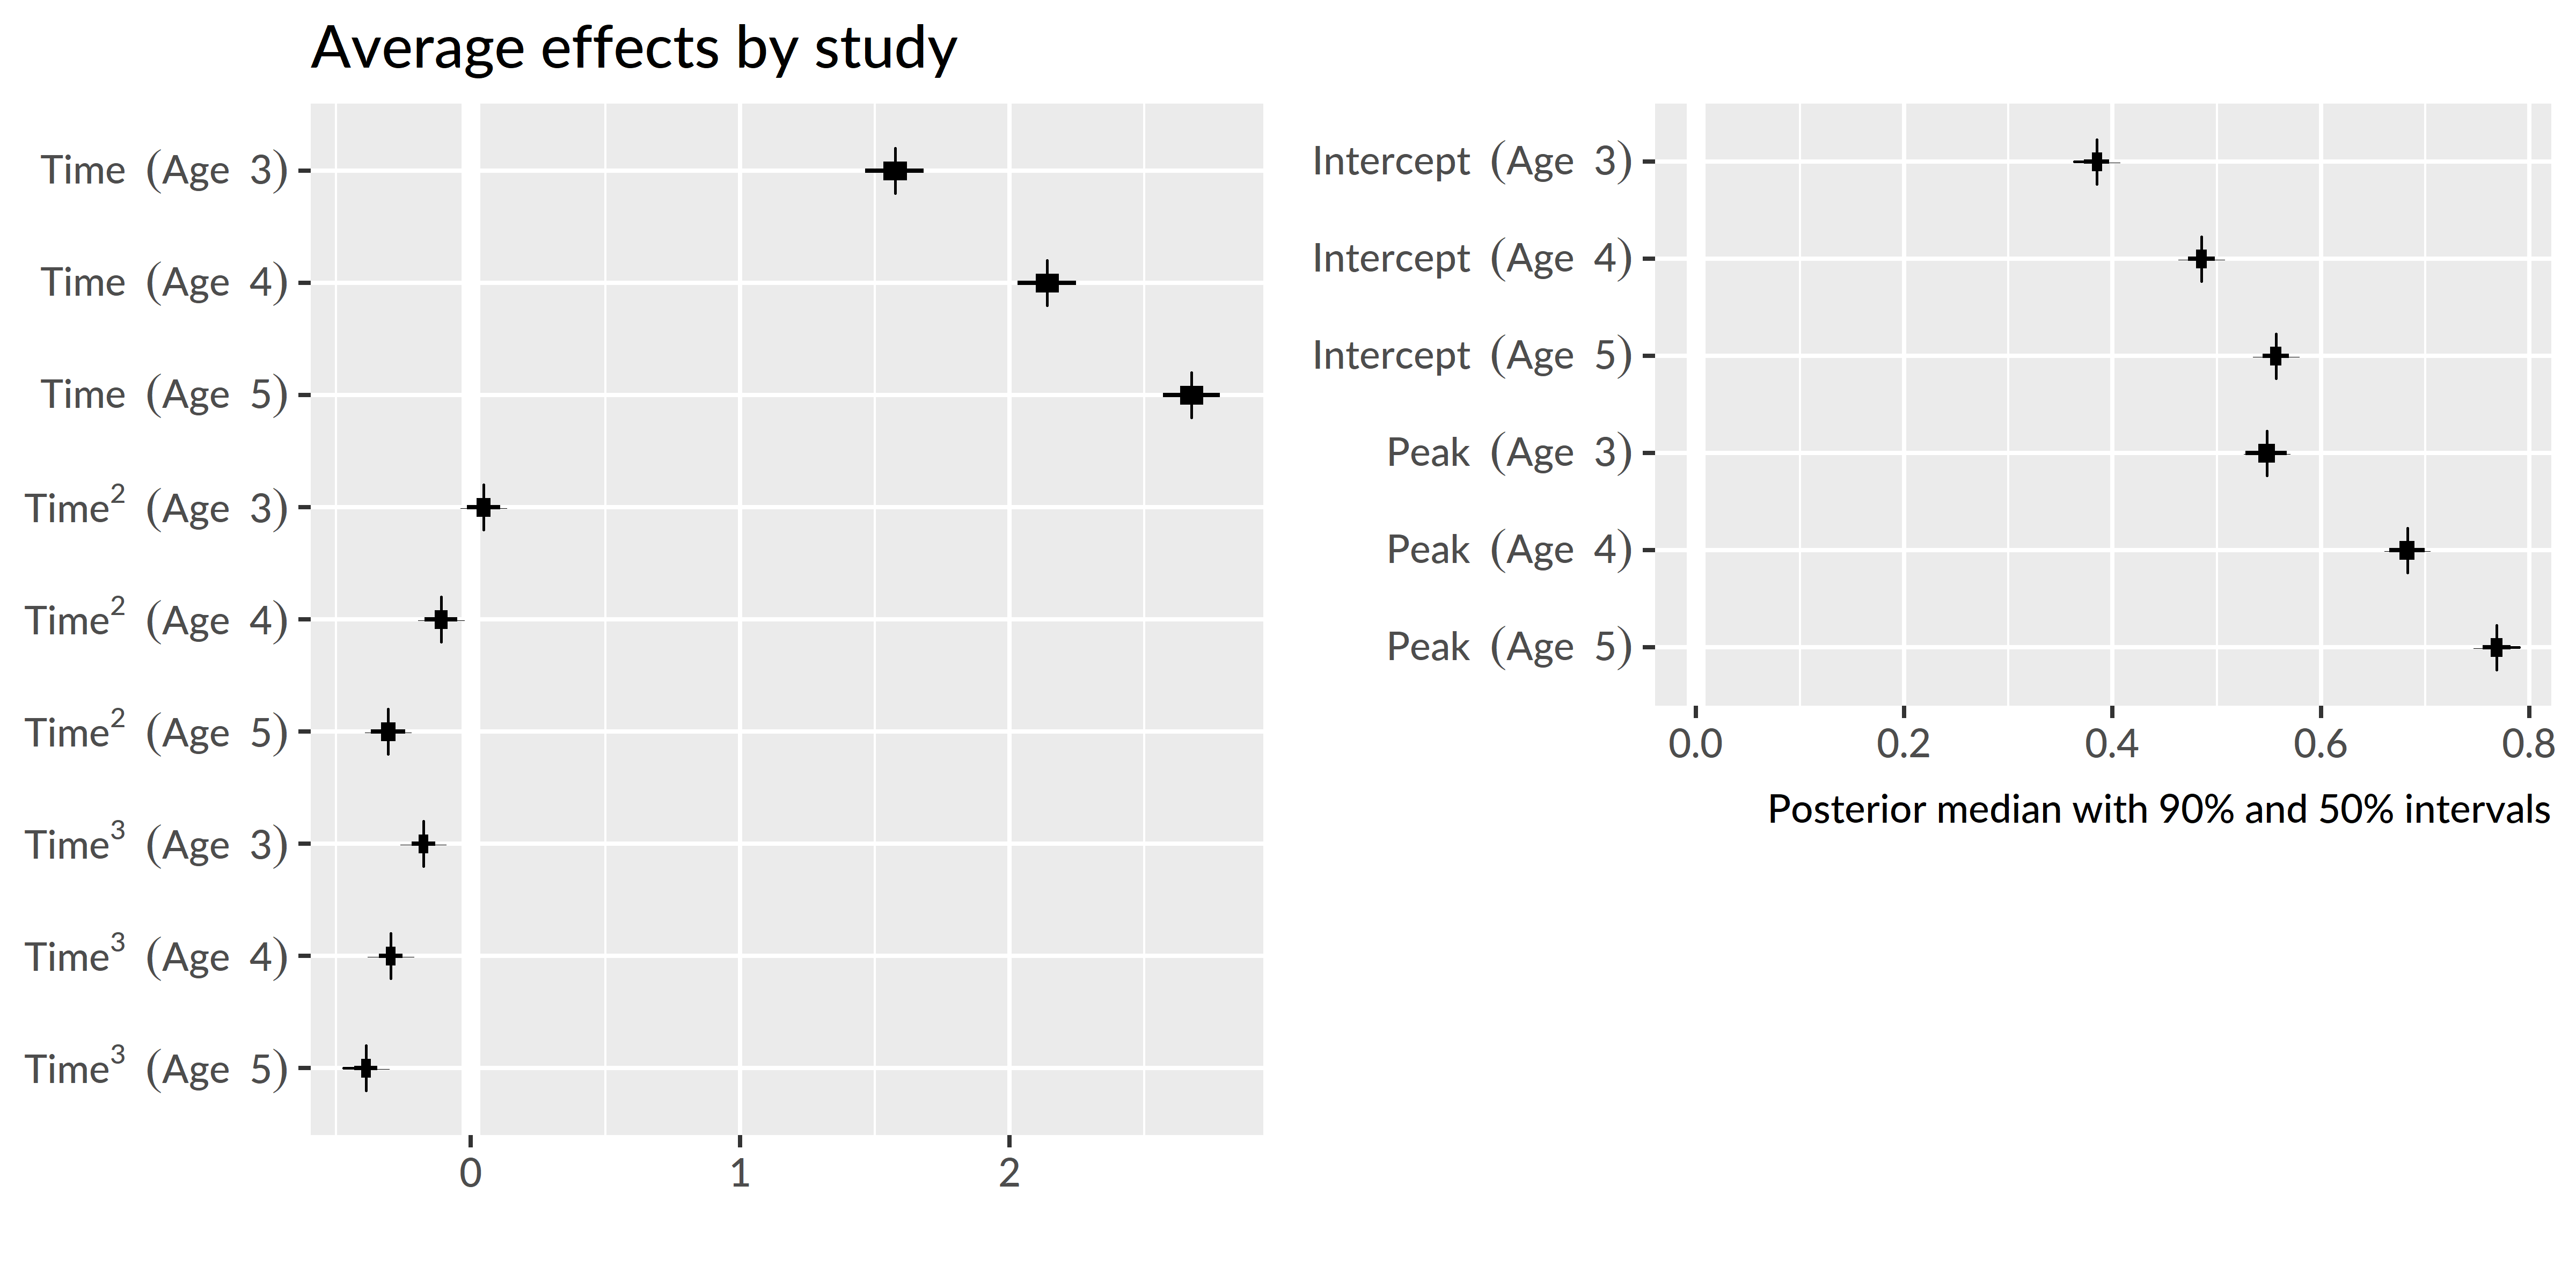
\includegraphics[width=0.8\linewidth]{14-aim1-familiar-word-recognition_files/figure-latex/effects2-1} \caption{Uncertainty intervals for the effects of study years on
growth curve features. The intercept and peak features were converted
from log-odds to proportions to ease interpretation.}\label{fig:effects2}
\end{figure}



\begin{figure}
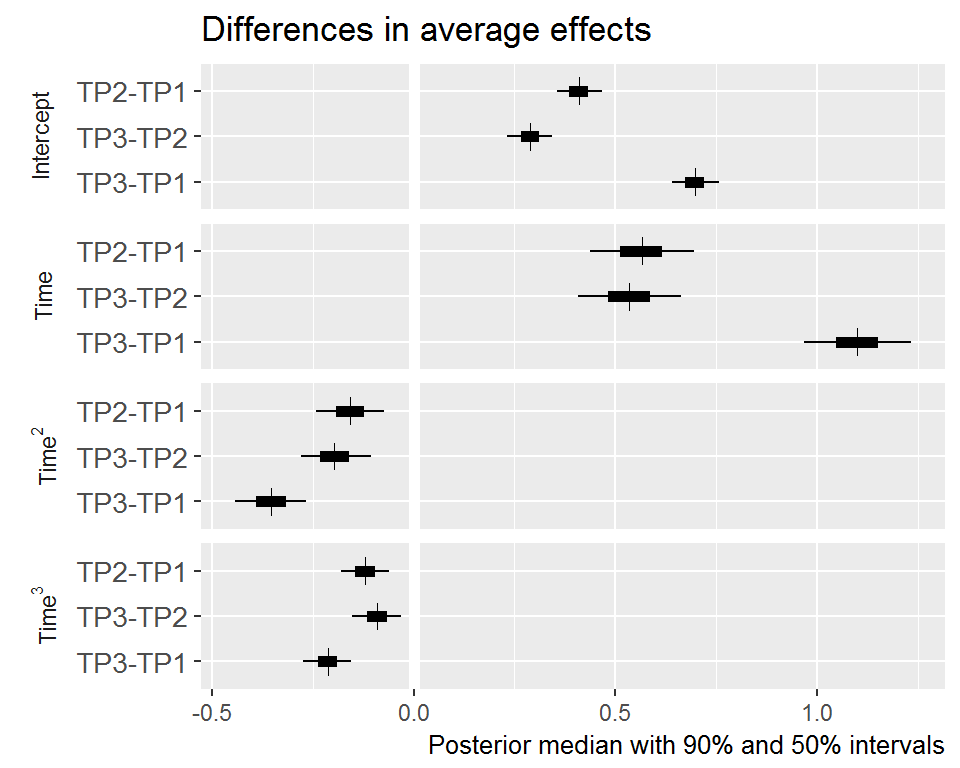
\includegraphics[width=0.5\linewidth]{14-aim1-familiar-word-recognition_files/figure-latex/pairwise-effects-1} 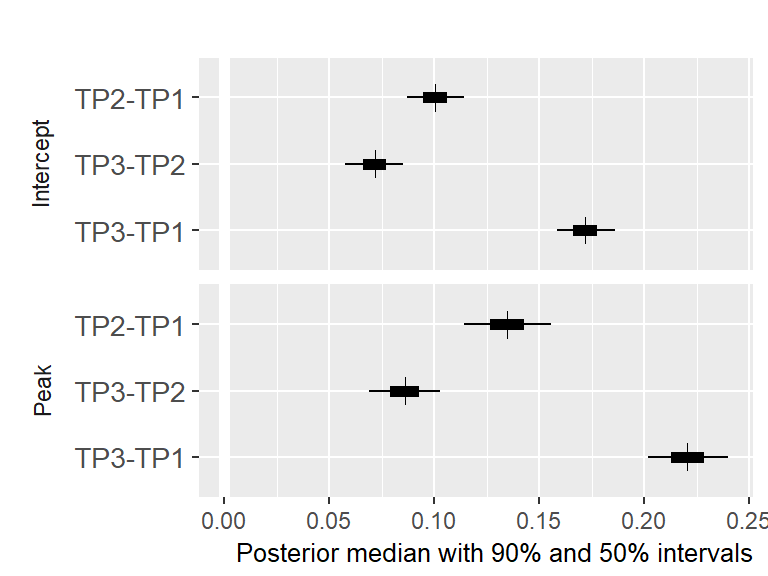
\includegraphics[width=0.5\linewidth]{14-aim1-familiar-word-recognition_files/figure-latex/pairwise-effects-2} \caption{Uncertainty intervals for the differences between
study timepoints. Again, the intercept and peak features were converted
to proportions.}\label{fig:pairwise-effects}
\end{figure}
The average looking probability (intercept feature) was 0.38 {[}90\% UI:
0.37--0.40{]} at age~3, 0.49 {[}0.47--0.50{]} at age~4, and 0.56
{[}0.54--0.57{]} at age~5. The averages increased by 0.10
{[}0.09--0.11{]} from age~3 to age~4 and by 0.07 {[}0.06--0.09{]} from
age~4 to age~5. The peak looking probability was 0.55 {[}0.53--0.57{]}
at age~3, 0.68 {[}0.67--0.70{]} at age~4, and 0.77 {[}0.76--0.78{]} at
age~5. The peak values increased by 0.13 {[}0.11--0.16{]} from age~3 to
age~4 and by 0.09 {[}0.07--0.10{]} from age~4 to age~5. These results
numerically confirm the hypothesis that children would improve in their
word recognition reliability, both in terms of average looking and in
terms of peak accuracy, each year.

\textbf{Summary}. The average growth curve features increased year over
year, so that children looked to the target more quickly and more
reliably.

\section{Exploring plausible ranges of performance over
time}\label{exploring-plausible-ranges-of-performance-over-time}

Bayesian models are generative; they describe how the data could have
been generated. This model assumed that each child's growth curve was
drawn from a population of related growth curves, and it tried to infer
the parameters over that distribution. These two aspects---a generative
model and learning about the population of growth curves---allow the
model to simulate new samples from that distribution of growth curves.
That is, we can predict a set of growth curves for a hypothetical,
unobserved child drawn from the same distribution as the 195 observed
children. This procedure allows one to explore the plausible degrees of
variability in performance at each age.

Figure \ref{fig:new-participants} shows the posterior predictions for
1,000 simulated participants, which demonstrates how the model expects
new participants to improve longitudinally but also exhibit stable
individual differences over time. Figure
\ref{fig:new-participants-intervals} shows uncertainty intervals for
these simulations. The model learned to predict less accurate and more
variable performance at age~3 with improving accuracy and narrowing
variability at age~4 and age~5.









\begin{figure}
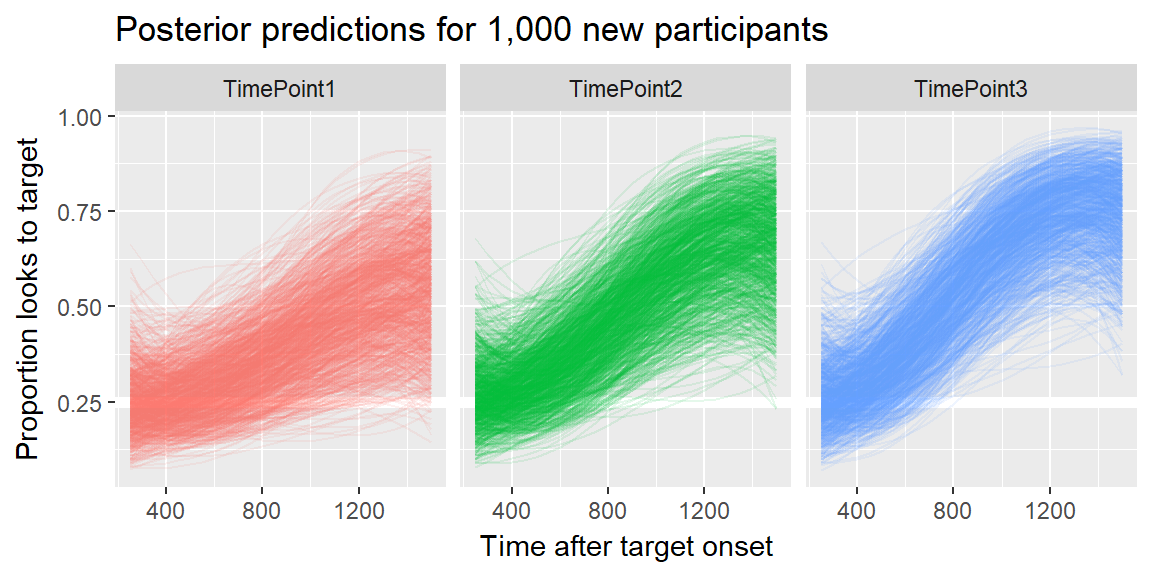
\includegraphics[width=0.8\linewidth]{14-aim1-familiar-word-recognition_files/figure-latex/new-participants-1} \caption{Posterior predictions for hypothetical
\emph{unobserved} participants. Each line represents the predicted
performance for a new participant. The three dark lines highlight
predictions from one single simulated participant. The simulated
participant shows both longitudinal improvement in word recognition and
similar relative performance compared to other simulations each year,
indicating that the model would predict new children to improve year
over year and show stable individual differences over time.}\label{fig:new-participants}
\end{figure}




\begin{figure}
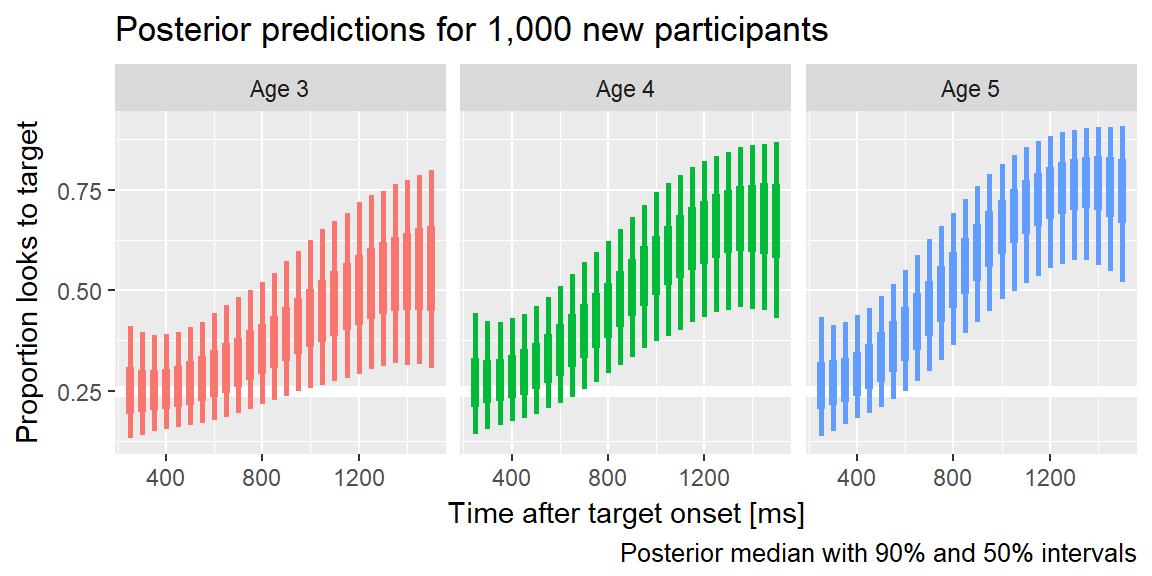
\includegraphics[width=0.8\linewidth]{14-aim1-familiar-word-recognition_files/figure-latex/new-participants-intervals-1} \caption{Uncertainty intervals for the simulated
participants. Variability is widest at age~3 and narrowest at age~5,
consistent with the prediction that children become less variable as
they grow older.}\label{fig:new-participants-intervals}
\end{figure}
I hypothesized that children would become less variable as they grew
older and converged on a mature level of performance. I address this
question by inspecting the ranges of predictions for the simulated
participants. The claim that children become less variable would imply
that the range of predictions should be narrower age~5 than for age~4
than age~3. Figure~\ref{fig:new-ranges} depicts the range of the
predictions, both in terms of the 90 percentile range (i.e., the range
of the middle 90\% of the data) and in terms of the 50 percentile
(interquartile) range. The ranges of performance decrease from age~3 to
age~4 to age~5, consistent with the hypothesized reduction in
variability.







\begin{figure}
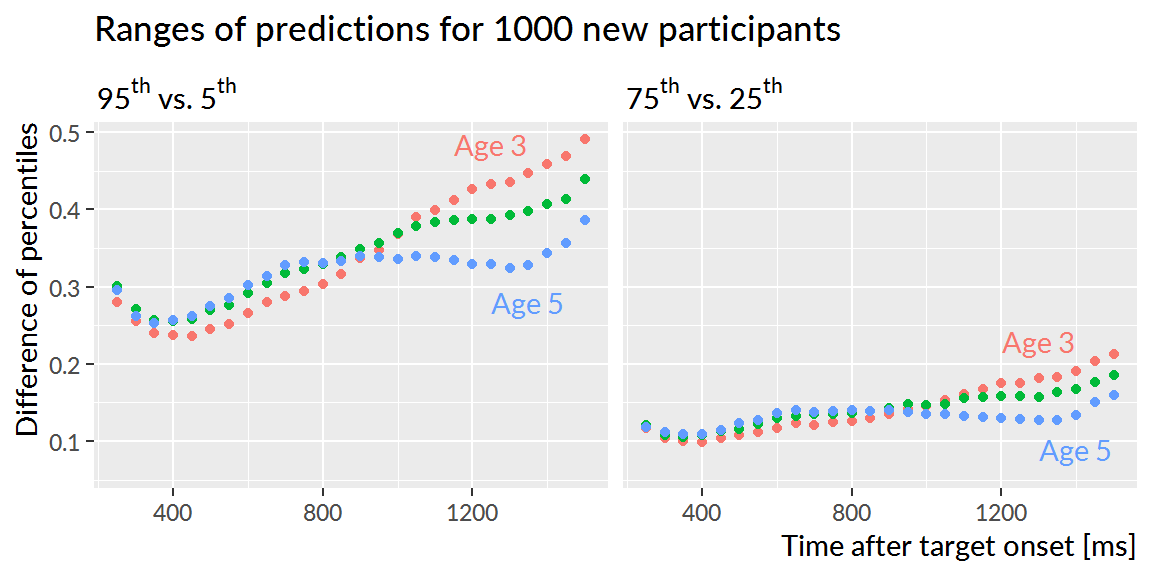
\includegraphics[width=0.8\linewidth]{14-aim1-familiar-word-recognition_files/figure-latex/new-ranges-1} \caption{Ranges of predictions for simulated participants over
the course of a trial. The ranges are most similar during the first half
of the trial when participants are at chance performance, and the ranges
are most different at the end of the trial as children reliably fixate
on the target image. The ranges of performance decreases with each year
of the study as children show less variability.}\label{fig:new-ranges}
\end{figure}
The developmental pattern of increasing reliability and decreasing
variability was also observed for the growth curve peaks. For the
synthetic participants, the model predicted that individual peak
probabilities will increase each year, peak3~= 0.55 {[}90\% UI:
0.35--0.77{]}, peak4~= 0.69 {[}0.48--0.86{]}, peak5~= 0.78
{[}0.59--0.91{]}. Moreover, the range of plausible values for the
individual peaks narrowed each for the simulated data. For instance, the
difference between the 95\textsuperscript{th} and 5\textsuperscript{th}
percentiles was 0.43 for age~3, 0.38 for age~4, and 0.32 for age~5.

\textbf{Summary}. I used the model's random effects estimates to
simulate growth curves from 1,000 hypothetical, unobserved participants.
The simulated dataset showed increasing looking probability and
decreasing variability with each year of the study. These simulations
confirmed the hypothesis that variability would be diminish as children
converge on a mature level of performance on this task.

\section{Are individual differences stable over
time?}\label{are-individual-differences-stable-over-time}

I predicted that children would show stable individual differences such
that children who are faster and more reliable at recognizing words at
age~3 remain relatively faster and more reliable at age~5. To evaluate
this hypothesis, I used Kendall's \emph{W} (the coefficient of
correspondence or concordance). This nonparametric statistic measures
the degree of agreement among \emph{J}~judges who are rating
\emph{I}~items. For these purposes, the items are the 123 children who
provided reliable eyetracking for all three years of the study. (That
is, I excluded children who only had reliable eyetracking data for one
or two years.) The judges are the sets of growth curve parameters from
each year of study. For example, the intercept term provides three sets
of ratings: The participants' intercept terms from year~1 are one set of
ratings and the terms from years~2 and~3 provide two more sets of
ratings. These three ratings are the ``judges'' used to compute the
intercept's \emph{W}. Thus, I computed five groups of \emph{W}
coefficients, one for each set of growth curve features: Intercept,
Time\textsuperscript{1}, Time\textsuperscript{2},
Time\textsuperscript{3}, and Peak looking probability.

Because I used a Bayesian model, there is a distribution of ratings and
thus a distribution of concordance statistics. Each sample of the
posterior distribution fits a growth curve for each child in each study,
so each posterior sample provides a set of ratings for concordance
coefficients. The distribution of \emph{W}'s lets us quantify our
uncertainty because we can compute \emph{W}'s for each of the 4000
samples from the posterior distribution.

One final matter is how to assess whether a concordance statistic is
meaningful. To tackle this question, I also included a ``null rater'', a
fake parameter that assigned each child in each year a random number. I
use the distribution of \emph{W}'s generated by randomly rating children
as a benchmark for assessing whether the other concordance statistics
differ meaningfully from chance.







\begin{figure}
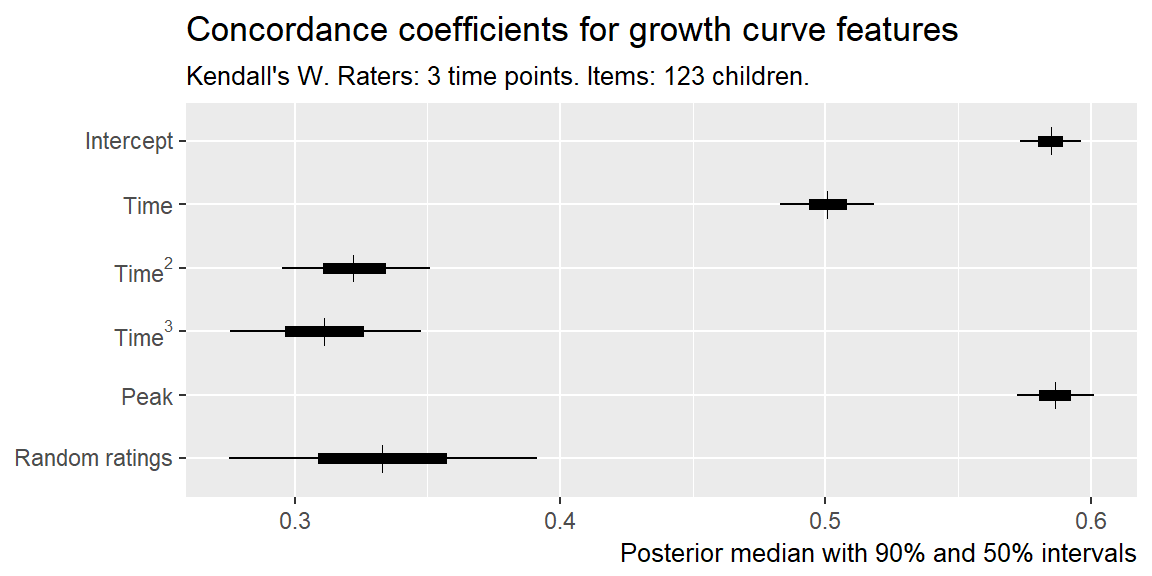
\includegraphics[width=0.8\linewidth]{14-aim1-familiar-word-recognition_files/figure-latex/kendall-stats-1} \caption{Uncertainty intervals for the Kendall's coefficient
of concordance. Random ratings provide a baseline of null \emph{W}
statistics. The intercept and linear time features are decisively
non-null, indicating a significant degree of correspondence in
children's relative word recognition reliability and efficiency over
three years of study.}\label{fig:kendall-stats}
\end{figure}
We used the \texttt{kendall()} function in the irr R package
(vers.~0.84; Gamer, Lemon, \& Singh, \protect\hyperlink{ref-irr}{2012})
to compute concordance statistics. Figure~\ref{fig:kendall-stats}
depicts uncertainty intervals for the Kendall \emph{W}'s for these
growth curve features. The 90\% uncertainty interval of \emph{W}
statistics from random ratings {[}0.28--0.39{]} subsumes the intervals
for the Time\textsuperscript{2} effect {[}0.30--0.35{]} and the
Time\textsuperscript{3} effect {[}0.28--0.35{]}, indicating that these
values do not differentiate children in a longitudinally stable way.
That is, the Time\textsuperscript{2} and Time\textsuperscript{3}
features differentiate children across studies as well as random
numbers. Earlier, I stated that only the intercept, linear time, and
peak features have psychologically meaningful interpretations and that
the higher-order features of these models serve to capture the shape of
the growth curve data. These concordance statistics support that
assertion.

Concordance is strongest for the peak feature, \emph{W}~= 0.59
{[}0.57--0.60{]} and the intercept term, \emph{W}~= 0.58
{[}0.57--0.60{]}, followed by the linear time term, \emph{W}~= 0.50
{[}0.48--0.52{]}. Because these values are far removed from the
statistics for random ratings, I conclude that there is a credible
degree of correspondence across studies when ranking children using
their peak looking probability, average look probability (the intercept)
or their growth curve slope (linear time).

\textbf{Summary}. Growth curve features reflected individual differences
in word recognition performance. By using Kendall's \emph{W} to measure
the degree of concordance among growth curve features over time, I
tested whether individual differences in lexical processing persisted
over development. I found that the peak looking probability, average
looking probability and linear time features were stable over time.

\section{Predicting future vocabulary
size}\label{predicting-future-vocabulary-size}

I hypothesized that individual differences in word recognition at age~3
will be more discriminating and predictive future language outcomes than
differences at age~4 or age~5. To test this hypothesis, we calculated
the correlations of growth curve features with age~5 expressive
vocabulary size and age~4 receptive vocabulary. (The receptive test was
not administered during the last year of the study for logistical
reasons.) As with the concordance analysis, I computed each of the
correlations for each sample of the posterior distribution to obtain a
distribution of correlations.

Figure~\ref{fig:evt2-gca-cors} shows the correlations of the peak
looking probability, average looking probability and linear time
features with expressive vocabulary size at age~5, and
Figure~\ref{fig:ppvt4-gca-cors} shows analogous correlations for the
receptive vocabulary at age~4. For all cases, the strongest correlations
were found between the growth curve features at age~3.

Growth curve peaks from age~4 correlated with age~5 vocabulary with
\emph{r}~= .52 {[}90\%~UI .50--.54{]}, but the concurrent peaks from
age~5 showed a correlation of just \emph{r}~= .31 {[}.29--.33{]}, a
difference between age~3 and age~5 of \emph{r}3−5~= .21 {[}.18--.24{]}.
A similar pattern held for lexical processing efficiency values. Linear
time features from age~3 correlated with age~5 vocabulary with
\emph{r}~= .41 {[}.39--.44{]}, whereas the concurrent lexical processing
values from age~5 only showed a correlation of \emph{r}~= .28
{[}.26--.31{]}, a difference of \emph{r}3−5~= .13 {[}.10--.16{]}. For
the average looking probabilities, the correlation for age~3, \emph{r}~=
.39 {[}.39--.44{]}, was probably only slightly greater than the
correlation for age~4, \emph{r}3−4~= .02 {[}−.01--.04{]} but
considerably greater than the concurrent correlation at age~5,
\emph{r}3−5~= .08 {[}.05--.10{]}.





\begin{figure}
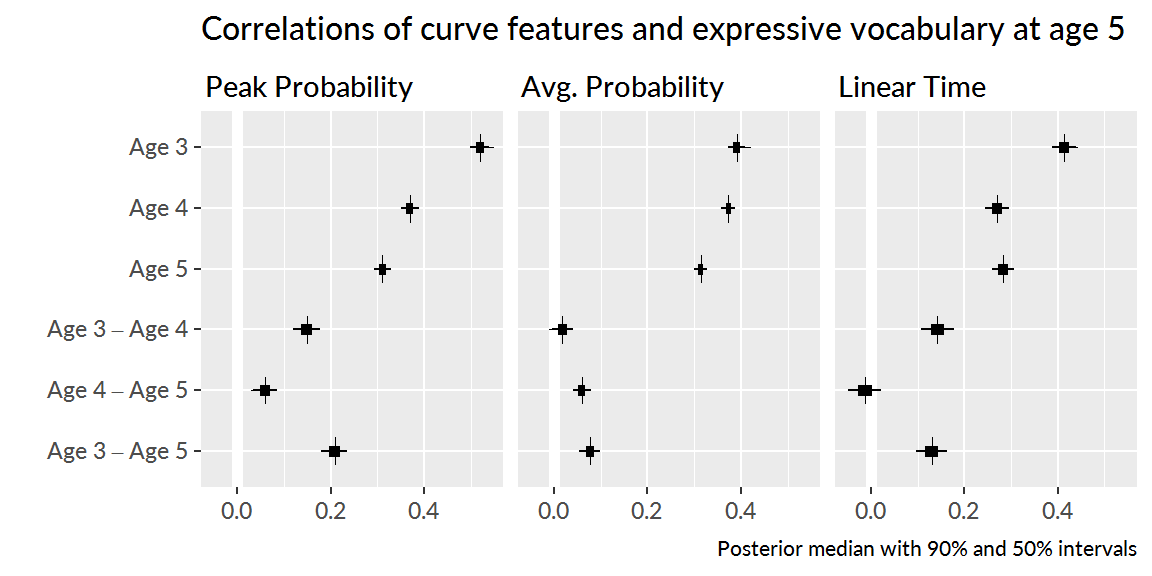
\includegraphics[width=0.8\linewidth]{14-aim1-familiar-word-recognition_files/figure-latex/evt2-gca-cors-1} \caption{Uncertainty intervals for the correlations of growth
curve features at each time point with expressive vocabulary (EVT-2
standard scores) at age~5. The bottom rows provide intervals for the
pairwise differences in correlations between timepoints.}\label{fig:evt2-gca-cors}
\end{figure}
Peak looking probabilities from age~3 were strongly correlated with
age~4 receptive vocabulary, \emph{r}~= .62 {[}.61--.64{]}, and this
correlation was much greater than the correlation observed for the age~4
growth curve peaks, \emph{r}3−4~= .26 {[}.26{]}. The correlation of
age~3 average looking probabilities, \emph{r}~= .45 {[}.44--.47{]}, was
greater than the age~4 correlation, \emph{r}3−4~= .08 {[}.06--.11{]},
and the correlation for age~3 linear time features, \emph{r}~= .51
{[}.49--.54{]}, was likewise greater, \emph{r}3−4~= .22 {[}.19--.26{]}.





\begin{figure}
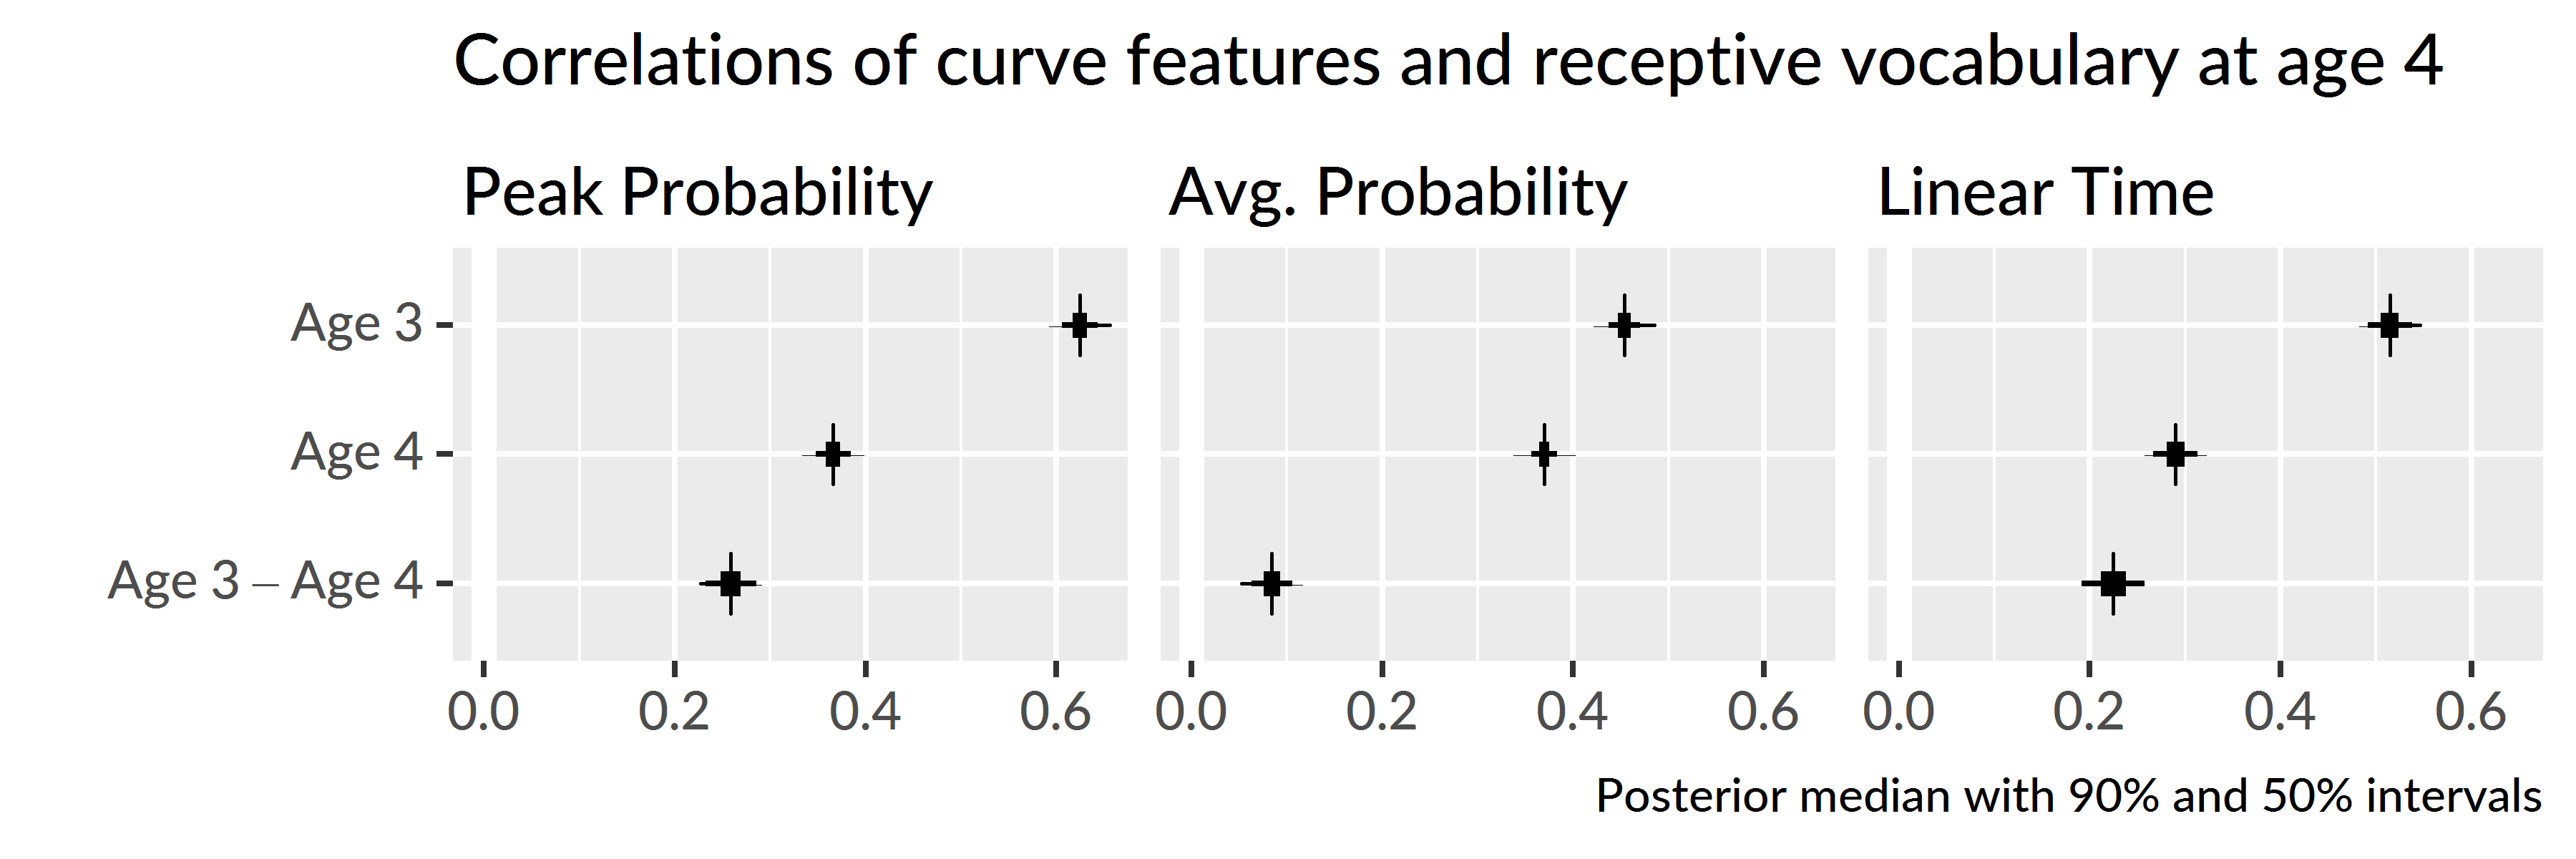
\includegraphics[width=0.8\linewidth]{14-aim1-familiar-word-recognition_files/figure-latex/ppvt4-gca-cors-1} \caption{Uncertainty intervals for the correlations of
growth curve features at each time point with expressive vocabulary
(PPVT-4 standard scores) at age~4. The bottom row shows pairwise
differences between the correlations from timepoints.}\label{fig:ppvt4-gca-cors}
\end{figure}
\textbf{Summary}. Although individual differences in word recognition
were stable over time, early differences were more significant than
later ones. The strongest predictors of future vocabulary size were the
growth curve features from age~3.

\section{Discussion}\label{discussion}

In the preceding analyses, I analyzed many aspects of children's
recognition of familiar words. First, I examined how children's looking
patterns \emph{on average} changed year over year. Children's word
recognition improved each year: The growth curves grew steeper, reached
higher peaks, and increased in their average value each year. This
result was unsurprising, but it was valuable because it confirmed that
this word recognition task scaled with development. The task was simple
enough that children could recognize words at age~3, but challenging
enough for children's performance to improve each year.

After establishing how the averages changed each year, I next asked how
variability changed each year. To tackle this question, I used posterior
predictive inference to have the model simulate samples of data, and in
particular, to simulate new participants. The range of performance
narrowed each year, so that children were most variable at age~3 and
least variable at age~5. This result is consistent with a model of
development children vary widely early on and converge on a more mature
level of performance. From this perspective, word recognition as a skill
is like articulation where most children grow out of immature speech
patterns by grade school. An alternative outcome would have been
troubling: Word recognition differences that expanded with age, the
emergence of a word recognition ``gap''.

Although the range of individual differences decreased with age,
individual differences did not disappear over time. When children at
each age were ranked using growth curve features, we found a high degree
of correspondence among these ratings. Children who were faster or more
accurate at age~3 remained relatively fast or accurate at age~5. Thus,
differences in word recognition were longitudinally stable over the
preschool years. Extrapolating forwards in time, these differences
likely would become smaller and smaller and become irrelevant for
everyday listening situations. It is conceivable, however, that
individual differences might re-emerge and differentiate word
recognition performance under adverse listening conditions.

Lastly, I analyzed how individual differences in word recognition
features correlated with future vocabulary outcomes. The peak looking
probabilities and growth curve slopes from age~3 showed the strongest
correlations with future vocabulary scores. This finding was remarkable:
Expressive vocabulary scores at age~5, for example, were more strongly
correlated with word recognition data collected two years earlier than
word recognition data collected during the same week.

We can understand this predictive value of age-3 word recognition from
two perspectives. The first is statistical. Differences in children's
word recognition performance were greatest at age~3, so word recognition
features at age~3 provide more variance and more information about the
children and their future vocabulary size. The second is conceptual.
Correlations were strongest for the growth curve peaks. We can think of
this feature as measuring children's maximum word recognition certainty.
A child with a peak of~.5, for example, looked the target image half of
the time when they were most certain about the word. Although all of the
words used were chosen to be familiar to preschoolers, children with
higher peaks knew those words \emph{better}. From the perspective,
higher peaks at age~3 would indicate more developed lexical
representations and stronger activation of lexical items at this age.
Thus, these children have a stronger foundation for word-learning than
children who show more uncertainty during word recognition.

\chapter{Effects of phonological and semantic
competitors}\label{effects-of-phonological-and-semantic-competitors}

\section{Looks to the phonological
competitor}\label{looks-to-the-phonological-competitor}

Next, I asked how children's sensitivity to the phonological foils
changed over developmental time. Following our approach in (Law et al.,
\protect\hyperlink{ref-RWLPaper}{2016}), I only examined trials for
which the phonological foil and the noun shared the same syllable onset.
For example, this criterion included trials with
\emph{dress}--\emph{drum}, \emph{fly}--\emph{flag}, or
\emph{horse}--\emph{heart}, but it excluded trials
\emph{kite}--\emph{gift} (feature difference), \emph{bear}--\emph{bread}
(onset difference), and \emph{ring}--\emph{swing} (rimes). I kept 13~of
the 24~trials. \protect\hyperlink{vw-experiment-items}{Appendix
\ref{vw-experiment-items}} provides a complete list of trials used.

The outcome measure for these analyses was the log-odds of fixating on
the phonological foil versus the unrelated image. Because children
looked more to the target word with each year of the study, they
necessarily looked less to the distractors each year.
Figure~\ref{fig:declining-phon-props} illustrates how the proportions of
looks to the phonological foils declined each year. Therefore, I
examined the effect of the phonological foil in comparison to the
unrelated foil. For example, on the trials where the target is
\emph{fly}, we can study the effect of the phonological foil \emph{flag}
by looking at when and to what to degree the children fixate on
\emph{flag} more than the unrelated image \emph{pen}. If a window of
time of shows a consistent advantage for the phonological foil over the
unrelated image, we can conclude that the children were sensitive to the
phonological foil. By studying the time course of fixations to the
phonological foil versus the unrelated image, we can identify when the
phonological foil affected word recognition most significantly.

As in the previous models, I downsampled the data into 50-ms (3-frame)
bins in order to smooth the data. I modeled the looks from~ to~~ms.
Lastly, I aggregated looks by child, study and time.





\begin{figure}
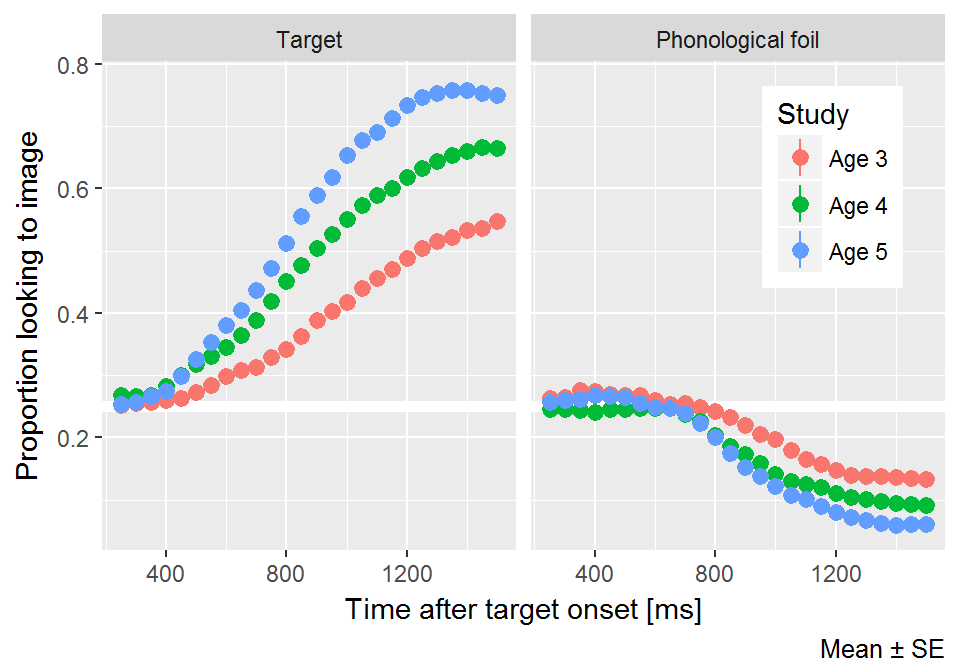
\includegraphics[width=0.6\linewidth]{16-aim1-lexical-competitors_files/figure-latex/declining-phon-props-1} \caption{Because children looked more to the target as
they grew older, they numerically looked less the foils too. This effect
is why I evaluated the phonological and semantic foils by comparing them
against the unrelated image.}\label{fig:declining-phon-props}
\end{figure}
To account for the sparseness of the data, I used the empirical log-odds
(or empirical logit) transformation (Barr,
\protect\hyperlink{ref-Barr2008}{2008}). This transformation adds .5 to
the looking counts. For example, a time-frame with 4 looks to the
phonological foil and 1 look to the unrelated image has a conventional
log-odds of log(4/1)~= 1.39 and empirical log-odds of log(4.5/1.5)~=
1.10. This transformation fills in 0 counts, and it dampens the
extremeness of some probabilities that arise in sparse count data.

To model these data, I fit a generalized additive model with fast
restricted maximum likelihood estimation (Sóskuthy,
\protect\hyperlink{ref-Soskuthy2017}{2017} for a tutorial for linguists;
Wood, \protect\hyperlink{ref-Wood2017}{2017}). Box~1 provides a brief
overview of these models. I used the mgcv R package (vers.~1.8.23; Wood,
\protect\hyperlink{ref-Wood2017}{2017}) with support from the tools in
the itsadug R package (vers.~2.3; van Rij, Wieling, Baayen, \& van Rijn,
\protect\hyperlink{ref-itsadug}{2017}).\footnote{Initially, I tried to
  use Bayesian polynomial growth curve models, as in the earlier
  analysis of the looks to the target image. These models however did
  not converge, even when strong priors were placed on the parameters.}

\Begin{infobox}

\textbf{Box 1: The Intuition Behind Generalized Additive Models}.

In these analyses, the outcome of interest is a value that changes over
time in a nonlinear way. We model these time series by building a set of
features to represent time values. In the growth curve analyses of
familiar word recognition, I used a set of polynomial features which
expressed time as the weighted sum of a linear trend, a quadratic trend
and cubic trend. That is:

\[
\text{log-odds}(\mathit{looking}) =
  \alpha + \beta_1 * \textit{Time}^1 +
           \beta_2 * \textit{Time}^2 +
           \beta_3 * \textit{Time}^3
\]

But another way to think about the polynomial terms is as \emph{basis
functions}: A set of features that combine to approximate some nonlinear
function of time. Under this framework, the model can be expressed as:

\[
\text{log-odds}(\mathit{looking}) =
  \alpha + f(\textit{Time})
\]

This is the idea behind generalized additive models and their
\emph{smooth terms}. These smooths fit nonlinear functions of data by
weighting and adding simple functions together. The figures below show 9
basis functions from a ``thin-plate spline'' and how they can be
weighted and summed to fit a growth curve.
\begin{center}\includegraphics[width=0.66\linewidth]{16-aim1-lexical-competitors_files/figure-latex/infobox-1-figs-1} \end{center}

Each of these basis functions is weighted by a model coefficient, but
the individual basis functions are not a priori meaningful. Rather, it
is the whole set of functions that approximate the curvature of the
data---i.e., \emph{f}(Time))---so we statistically evaluate the whole
batch of coefficients simultaneously. This joint testing is similar to
how one might test a batch of effects in an ANOVA. If the batch of
effects jointly improve model fit, we infer that there is a significant
smooth or shape effect.

Smooth terms come with an estimated degrees of freedom (EDF). These
values provide a sense of how many degrees of freedom the smooth
consumed. An EDF of~1 is a perfectly straight line, indicating no
smoothing. Higher EDF values indicate that the smooth term captured more
curvature from the data.

\End{infobox}

The model included main effects of study year. These \emph{parametric}
terms work like conventional regression effects and determined the
growth curve's average values. The model used age~4 as the reference
year, so the intercept represented the average looking probability at
age~4. The model's year effects therefore represented differences
between age 4~vs.~age~3 and age~4 vs.~age~5.

The model also included \emph{smooth} terms to represent the time course
of the data. As with the parametric effects, age~4 served as the
reference year. The model estimated a smooth for age~4 and it estimated
\emph{difference smooths} to capture how the curvature at age~3 and
age~5 differed from the age-4 curvature. Each of these study-level
smooths used 10 knots (9 basis functions). I also included child-level
\emph{random smooths} to represent child-level variation in growth curve
shapes. Because there is much as less data at the child level than at
the study level, these random smooths only included 5 knots (4 basis
functions). We can think of these simpler splines as coarse adjustments
in growth curve shape to capture child-level variation from limited
data. Altogether, the model contained the following terms:

\small
\begin{align*}
   \text{emp. log-odds}(\mathit{phon.\ vs.\ unrelated}) =\
   & \alpha + \beta_1\text{Age3} + \beta_2\text{Age5} +\ &\text{[growth curve averages]} \\
   & f_1(\text{Time}, \text{Age4})\ +                    &\text{[reference smooth]} \\
   & f_2(\text{Time}, \text{Age4} - \text{Age3})\ +      &\text{[difference smooths]} \\
   & f_3(\text{Time}, \text{Age4} - \text{Age5})\ +      & \\
   & f_i(\text{Time}, \text{Child}_i)                    &\text{[by-child random smooths]} \\
\end{align*}
The model's fitted values are shown in
Figure~\ref{fig:phon-vs-unre-fits}. These are the average empirical
log-odds of fixating on the phonological foil versus the unrelated image
for each year of the study. The model captured the trend for increased
looks to the competitor image with each year of the study. At age~4 and
age~5, the shape rises from a baseline to the peak around 800~ms. These
curves slope downwards and eventually fall beneath the initial baseline.
The shape at age~3 does not have a steady rise from baseline and shows a
very small peak around 800~ms.







\begin{figure}
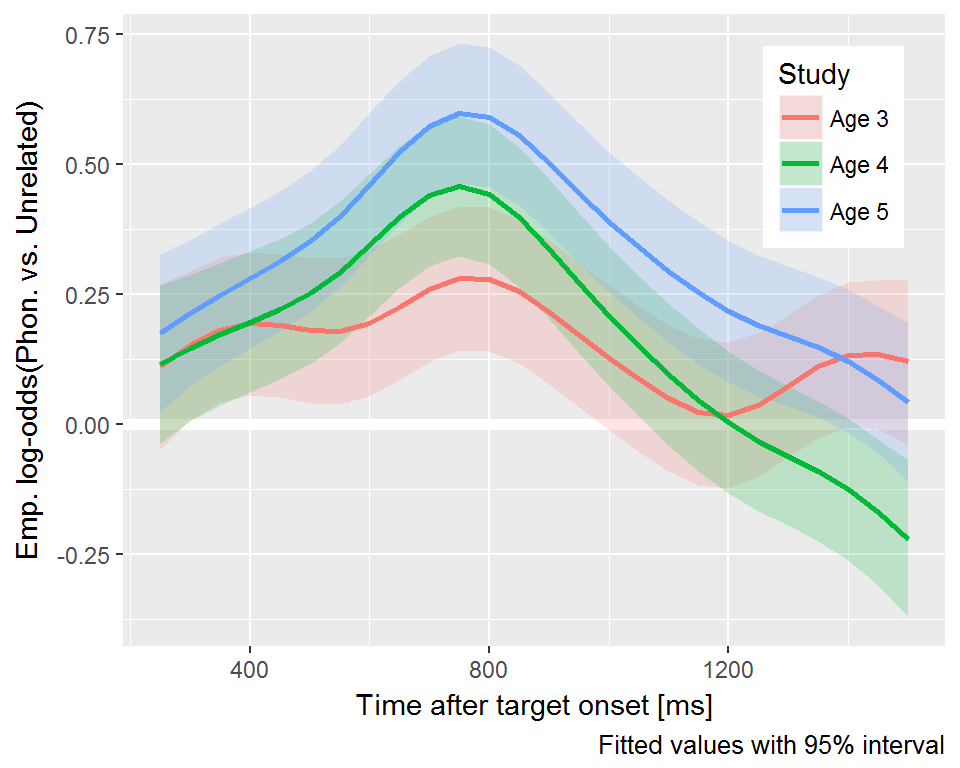
\includegraphics[width=0.8\linewidth]{16-aim1-lexical-competitors_files/figure-latex/phon-vs-unre-fits-1} \caption{With each year of the study, children looked
more to the phonological competitor, relative to the unrelated image,
during and after the target noun. Both figures show means for each year
estimated by the generalized additive model. The left panel compares
model estimates to observed means and standard errors, and the right
panel visualizes estimated means and their 95\% confidence intervals.}\label{fig:phon-vs-unre-fits}
\end{figure}
The average looks to the phonological foil over the unrelated for age~4
was 0.16 emp. log-odds, .54 proportion units. The averages for age~3 and
age~4 did not significantly differ, \emph{p}~= .85 but the average value
was significantly greater at age~5, 0.31 emp. log-odds, .58 proportion
units, \emph{p}~\textless{} .001. Visually, this effect shows up in the
almost constant height difference between the age-4 and the age-5
curves.









\begin{figure}
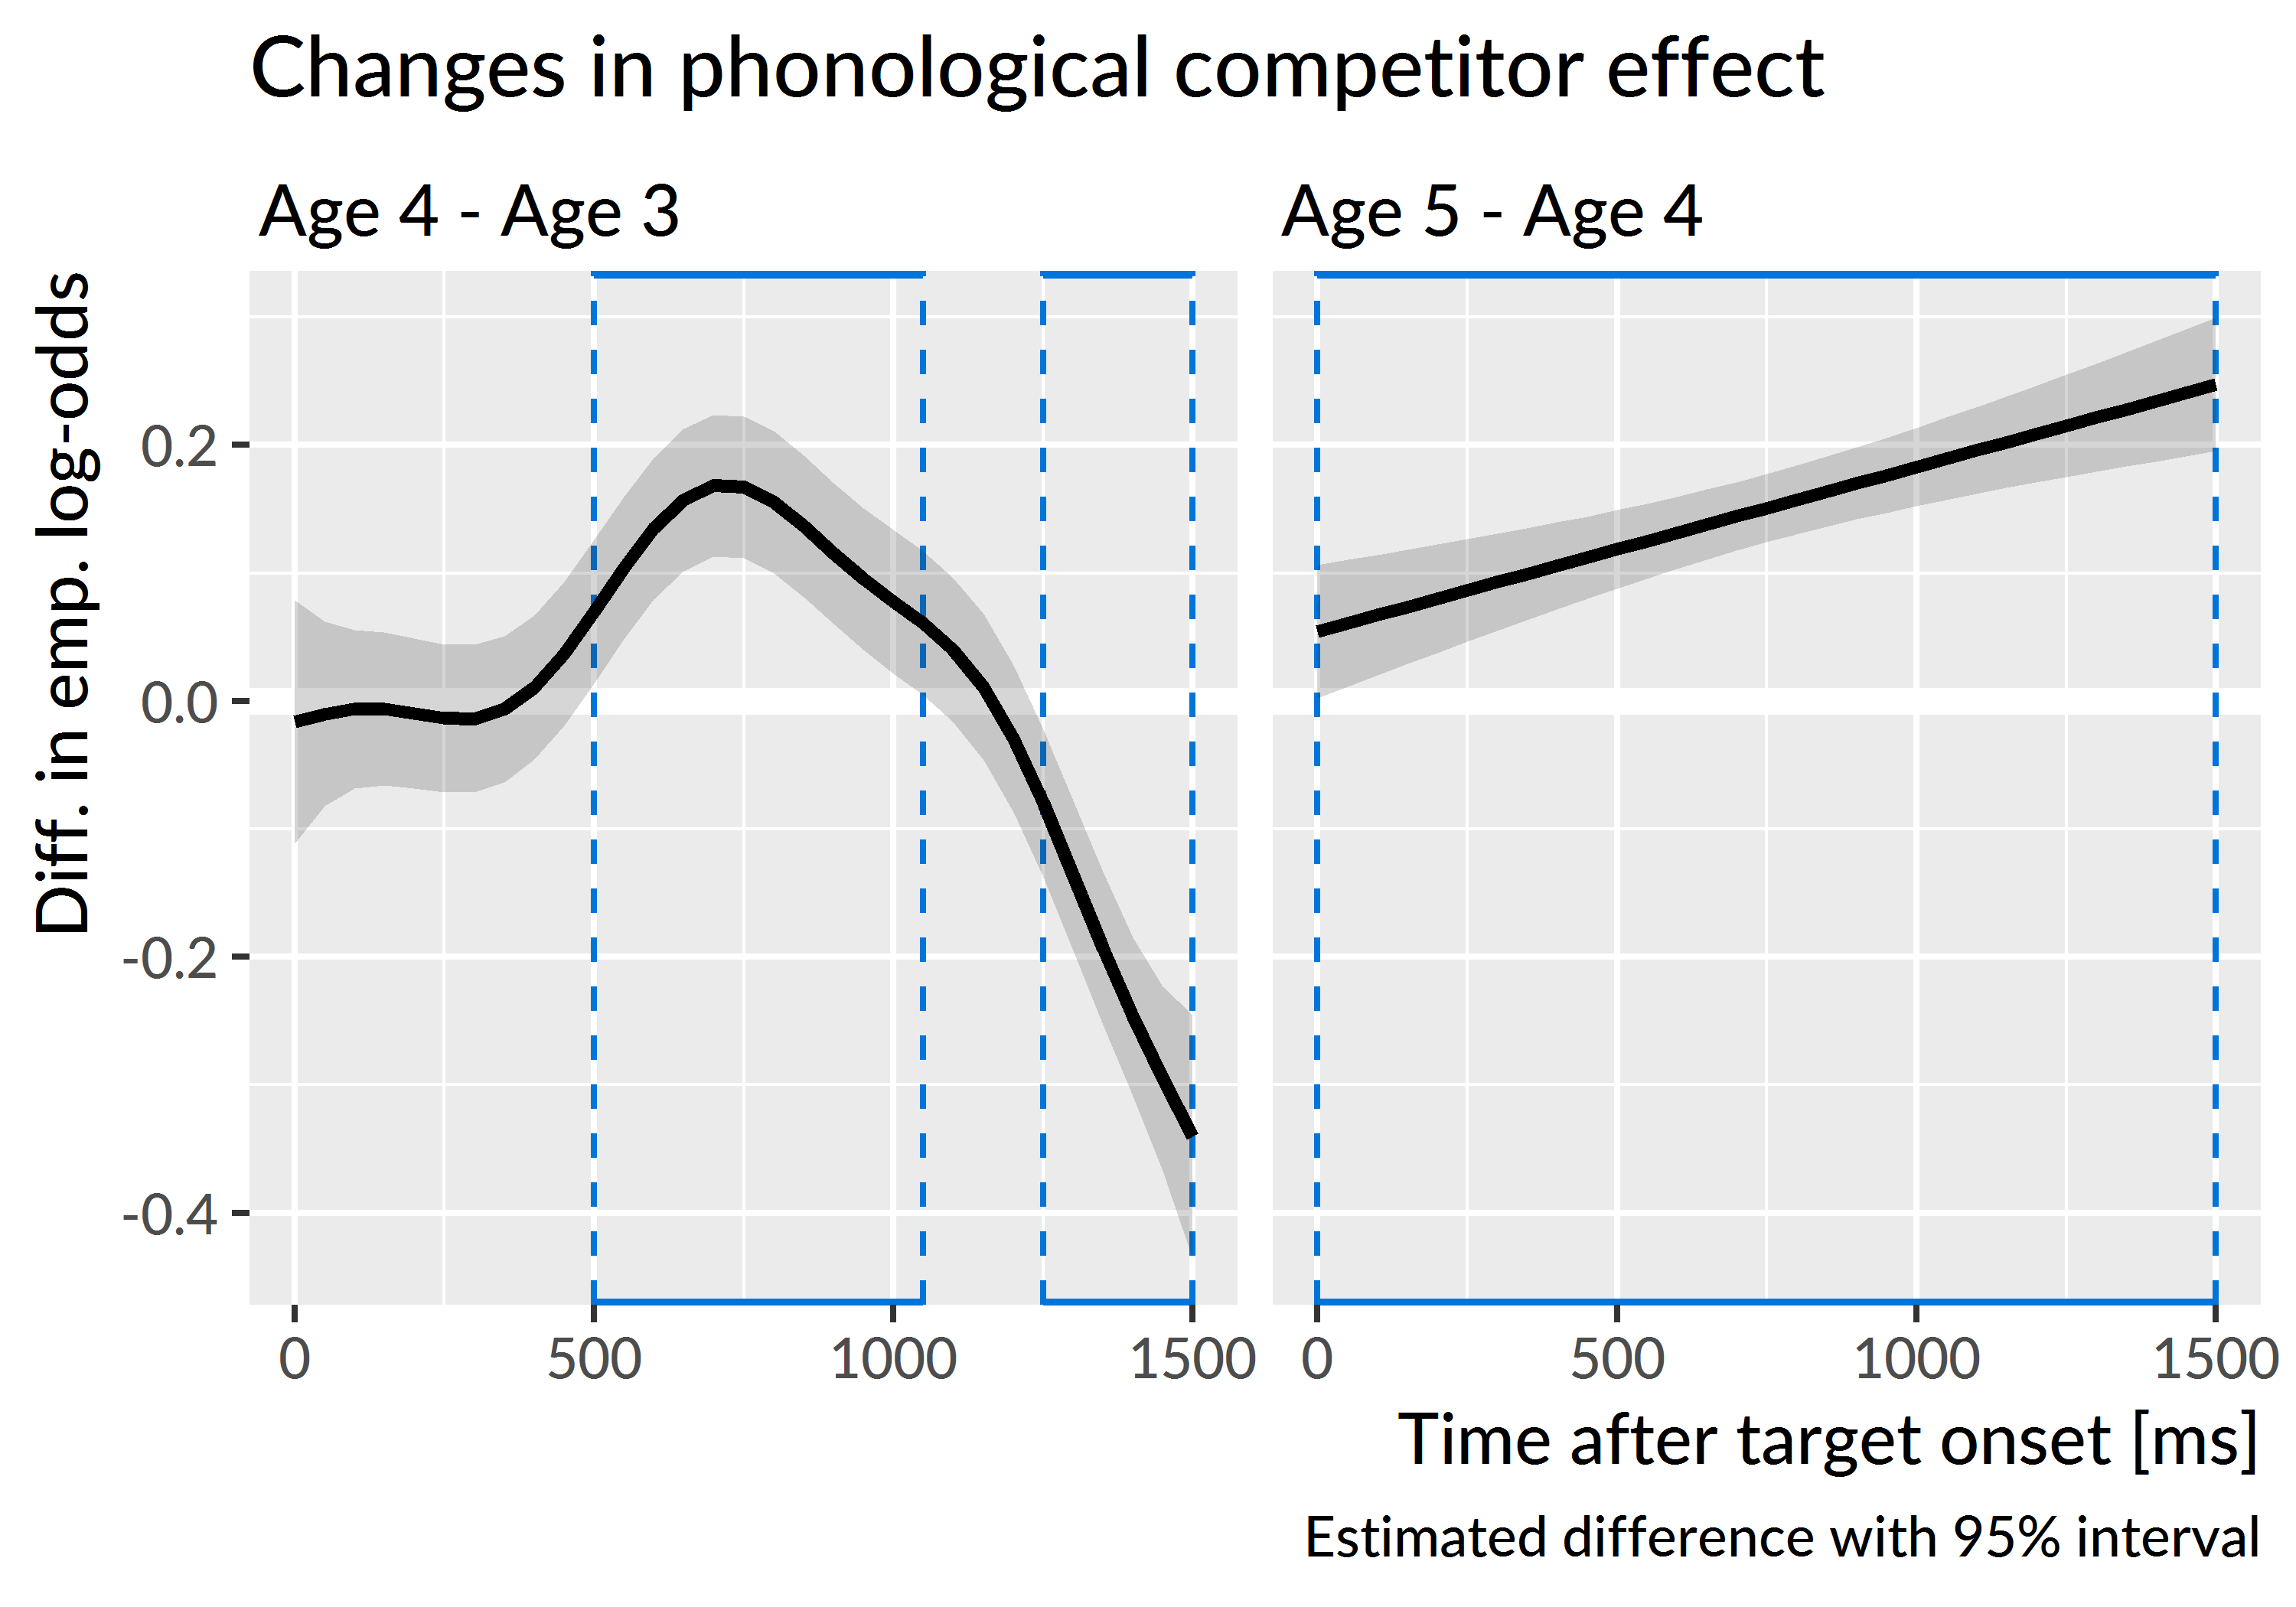
\includegraphics[width=0.8\linewidth]{16-aim1-lexical-competitors_files/figure-latex/phon-diff-curves-1} \caption{Differences in the average looks to the
phonological competitor versus the unrelated image between age~4 and the
other ages. Plotted line is estimated difference and the shaded region
is the 95\% confidence interval around that difference. Blue boxes
highlight regions where the 95\% interval excludes zero. From age~3 to
age~4, children become more sensitive to the phonological foil during
and after the target noun. The curves for age~3 and age~4 have largely
the same shape, but they steadily diverge over time.}\label{fig:phon-diff-curves}
\end{figure}
There was a significant smooth term for time at age~4, estimated degrees
of freedom (EDF)~= 7.28, \emph{p}~\textless{} .001.
Figure~\ref{fig:phon-diff-curves} visualizes how and when the smooths
from other studies differed from the age-4 smooth.

The age-3 and age-4 significantly differed, EDF~= 5.48,
\emph{p}~\textless{} .001. In particular, the curves are significantly
different from 500 to 1050~ms. This result confirms that the looks to
the phonological foil increased from age~3 and age~4 during the time
window immediately following presentation of the noun. The similarity
between the phonological foil and the target occurs early in the trial.
Given the 150--300~ms time required to execute an eye movement in
response to speech, the time window for these differences indicates that
children became more sensitive to the phonological similarities between
the foil and the target from age~3 to age~4.

The age-3 and age-4 curves also differed significantly after 1250~ms.
The effect reflects how the looks to phonological foil decreased as the
trial progresses. After an incorrect look to the foil, the children on
average corrected their gaze and looked even less to the phonological
foil. We do not observe this degree of correction during age~3,
presumably because children at age~3 hardly looked to the phonological
foil early on.

The age-4 and age-5 smooths also significantly differed, EDF~= 1.00,
\emph{p}~\textless{} .001, although the low EDF values indicates that
the shape of the difference was a flat line. Thus, the difference
between the age-4 and age-5 smooths is driven primarily by the intercept
difference and a linear diverging trend---that is, the distance between
the two grows slightly over time. The same general curvature was
observed for the two studies, reflecting the same general looking
behavior at both time points. Children showed an early increase in looks
to the phonological foil relative to the unrelated image but after
receiving disqualifying information from the rest of the word, the looks
to the phonological foil rapidly decrease. The primary difference
between age-4 and age-5 is that the foil effect becomes more pronounced
at age~5.

\textbf{Summary}. Children looked more the phonological competitor than
the unrelated image early in the trials. The advantage of the
phonological competitor peaked on average around 800~ms after target
onset. This peak was very small at age 3 but increased in height with
each year of the study. Thus, children became more sensitive to the
phonological cohort competitors as they grew older.

\section{Looks to the semantic
competitor}\label{looks-to-the-semantic-competitor}

I asked how children's sensitivity to the semantic competitor changed as
they grew older. As in (Law et al.,
\protect\hyperlink{ref-RWLPaper}{2016}), I only examined trials for
which the semantic foil and the noun were part of the same category. For
example, I included trials with \emph{bee}--\emph{fly},
\emph{shirt}--\emph{dress}, and \emph{spoon}--\emph{pan}, but I excluded
trials where the similarity was perceptual (\emph{sword}--\emph{pen}) or
too abstract (\emph{swan}--\emph{bee}). This criterion kept 13~of the
24~trials. \protect\hyperlink{vw-experiment-items}{Appendix
\ref{vw-experiment-items}} provides a complete list of trials used.

For these trials, I used the same modeling technique as the one used for
phonological competitor: Generalized additive models with study effects
and a time smooth, time-by-study difference smooths, and time-by-child
random smooths. I modeled the looks from from~250 to~1800~ms. This
window was 300~ms longer than the one used for the phonological
competitors in order to capture late-occurring semantic effects.

The model's fitted values are shown in
Figure~\ref{fig:semy-vs-unre-fits}. The average empirical log-odds of
fixating on the semantic foil versus the unrelated image increased with
each year of the study. All three years show the same general time
course of effects: Looks begin to increase from a baseline around 750~ms
and peak around 1300~ms. The peaks of the curves increased as children
grew older. The semantic foil shows a clear advantage over the unrelated
image at age~3, which was not the case for the phonological foil at
age~3.








\begin{figure}
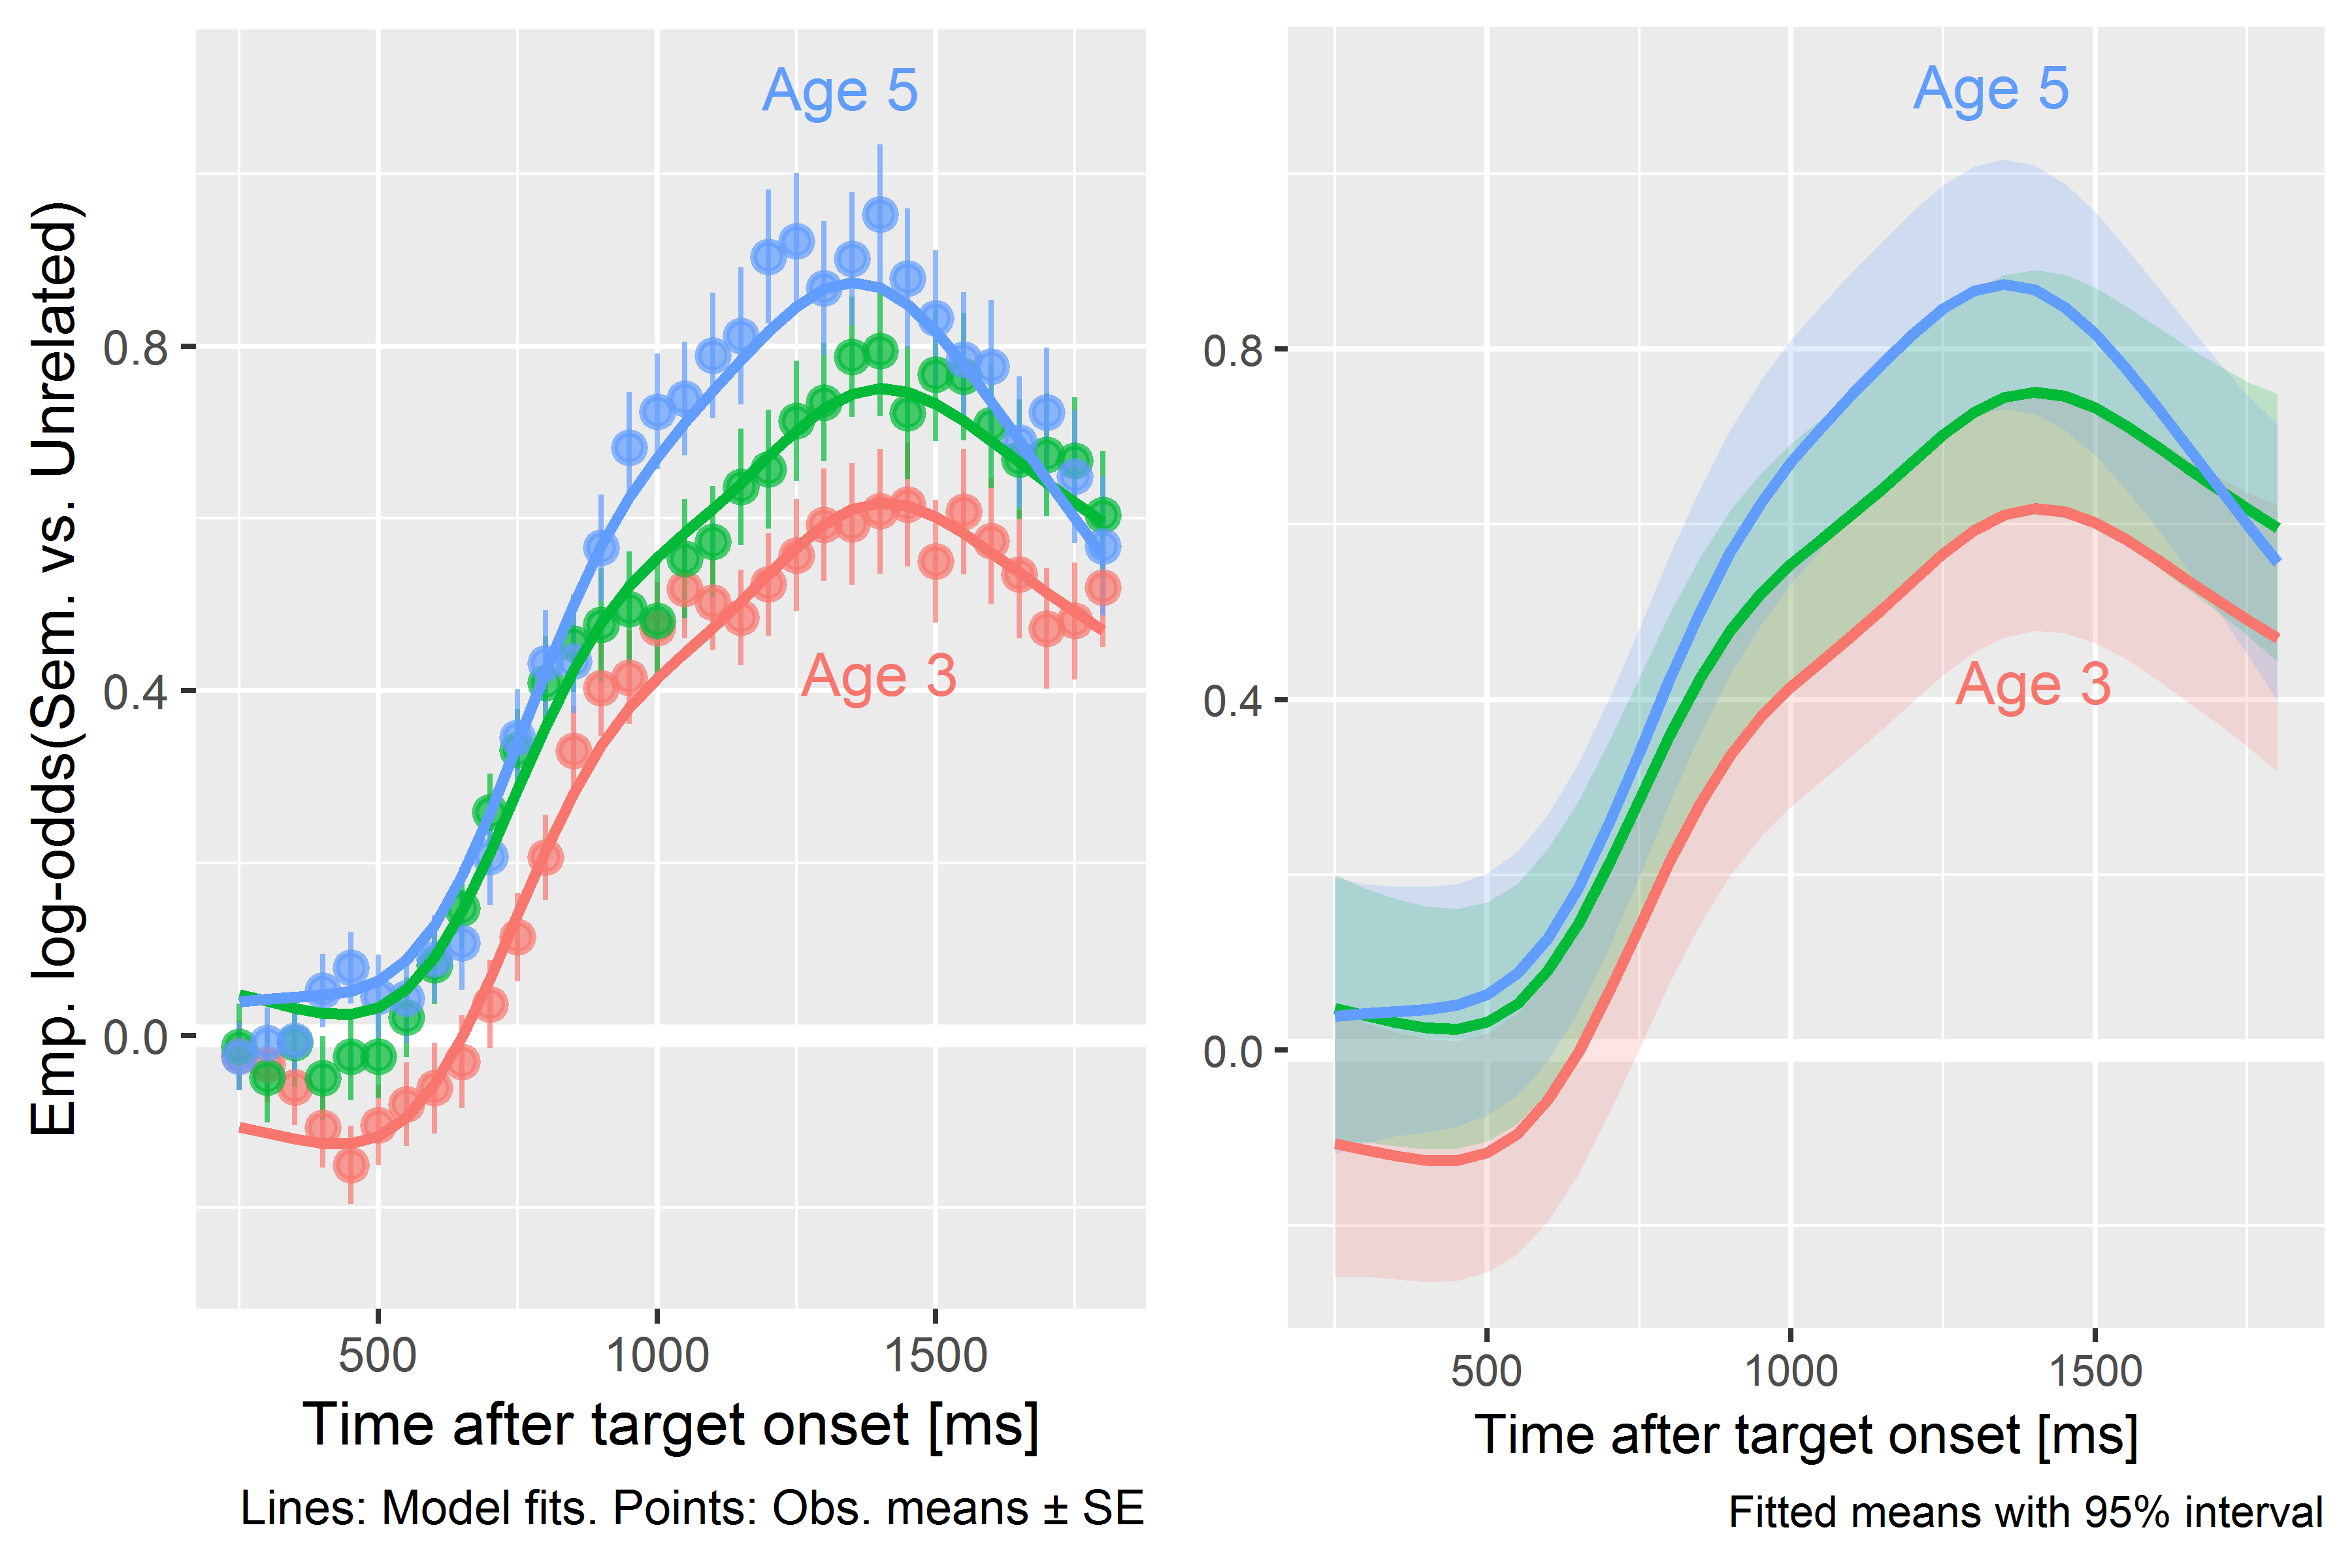
\includegraphics[width=0.8\linewidth]{16-aim1-lexical-competitors_files/figure-latex/semy-vs-unre-fits-1} \caption{With each year of the study, children looked
more to the semantic foil, relative to the unrelated image, with peak
looking occurring after the target noun. Both figures show means for
each year estimated by the generalized additive model. The left panel
compares model estimates to observed means and standard errors, and the
right panel visualizes estimated means and their 95\% confidence
intervals.}\label{fig:semy-vs-unre-fits}
\end{figure}
The average looks to the semantic foil over the unrelated for age~4 was
0.44 emp. log-odds, .61 proportion units. Children looked significantly
less to the semantic foil on average at age~3, 0.30 emp. log-odds, .57
proportion units, \emph{p}~\textless{} .001, and they looked
significantly more to the semantic foil at age~5, 0.50 emp. log-odds,
.62 proportion units, \emph{p}~\textless{} .001. The peaks of the growth
curves, in proportion units, were .65 at age~3, .68 at age~4, and .70 at
age~5.

There was a significant smooth term for time at age~4, estimated degrees
of freedom (EDF)~= 7.04, \emph{p}~\textless{} .001.
Figure~\ref{fig:semy-diff-curves} visualizes the time course of the
differences between the smooths from each study.









\begin{verbatim}
#> Summary:
#>  * Time : numeric predictor; with 32 values ranging from 250.000000 to 1800.000000. 
#>  * R : factor; set to the value(s): 001L. (Might be canceled as random effect, check below.) 
#>  * NOTE : The following random effects columns are canceled: s(Time,R)
#> 
\end{verbatim}
\begin{figure}
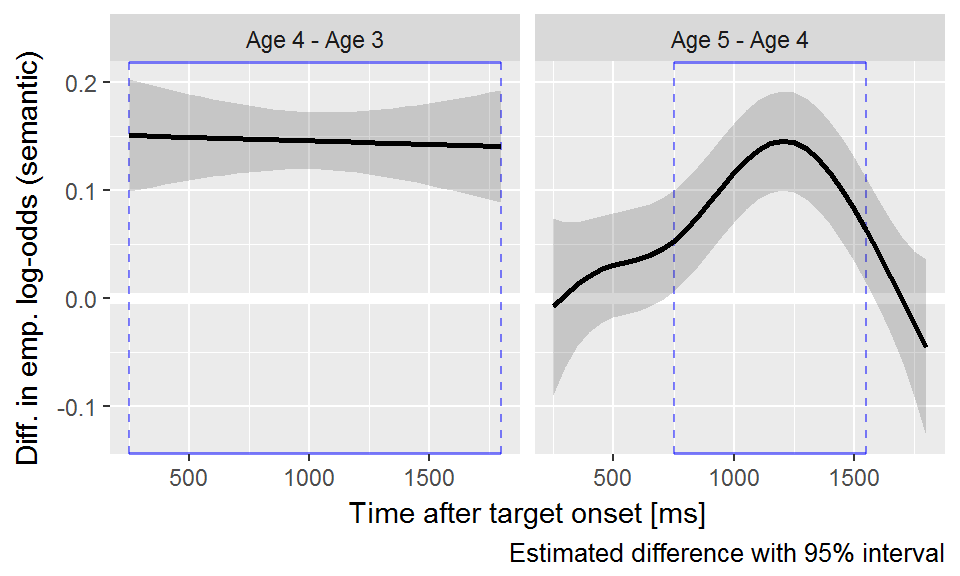
\includegraphics[width=0.8\linewidth]{16-aim1-lexical-competitors_files/figure-latex/semy-diff-curves-1} \caption{Differences in the average looks to the semantic
foil versus the unrelated image between age~4 and the other ages.
Plotted line is estimated difference and the shaded region is the 95\%
confidence interval around that difference. Blue boxes highlight regions
where the 95\% interval excludes zero. The flat line on the left
reflects how the shape of the growth curves remained the same from~age~3
to~age~4 and only differed in average height. From~age~4 to~age~5, the
lines quickly diverge and the age-5 curve reaches a higher peak value.}\label{fig:semy-diff-curves}
\end{figure}
The shapes of the age-3 and age-4 curves did not significantly differ,
EDF~= 1.00, \emph{p}~= .535. The age-3 curve begins to rise about 100~ms
later, and it reaches a shallower peak value than the age-4 curve. These
two features create a nearly constant height difference between the two
curves, and thus, the two curves show the same overall shape.

The age-4 and age-5 smooths significantly differed, EDF~= 1.00,
\emph{p}~\textless{} .001. The differences are greatest after the end of
the target noun, in the window from~750 to~1500~ms. The two curves start
from a similar baseline but quickly diverge as the age-5 curve reaches a
higher peak value. After 1500~ms, the age-5 curve turns downwards to
overlap with the age-4 curve. Thus, children looked more to the semantic
foil relative to the unrelated image, but they were also quicker to
correct and look away from it.

\textbf{Summary.} Children became more sensitive to the semantic
competitor, compared to the unrelated image, with each year of the
study. The semantic foils clearly influenced looking patterns at age~3,
in contrast to the muted effect observed for the phonological foils. The
semantic effect also occurred when we would expect: After the end of the
target noun, following activation of the target noun and its semantic
neighbors.

\section{Differences in competitor sensitivity at age
3}\label{differences-in-competitor-sensitivity-at-age-3}

Next, I asked whether children differed reliably in their sensitivity to
the phonological and semantic foils based on speech perception and
vocabulary measures collected at age~3

As a measure of speech perception, I used scores from a minimal pair
discrimination experiment administered during the first year of the
study. {[}citations{]} The task is essentially an ABX discrimination
task: A picture of a familiar object is shown and labeled (e.g.,
``car''), another object is shown and labeled (``jar''), and then both
images are shown and one of the two is named. The child then indicated
which word they heard by tapping on the image on a touch-screen.

I derived speech perception scores by fitting a hierarchical
item-response model. This logistic regression model estimates the
probability of child \emph{i} correctly choosing word \emph{j} on
word-pair \emph{k}. The equation below provides a term-by-term
description of the model. The model's intercept term represents the
average participant's probability of correctly answering for an average
item. By-child random intercepts capture a child's deviation from the
overall average, so they estimate the child's \emph{ability}. By-word
and by-word-in-pair random intercepts capture the relative difficulty of
particular items on the experiment. The by-word-in-pair effects were
necessary because four words appeared in more than one word pair (e.g.,
\emph{juice}--\emph{goose} and \emph{juice}--\emph{moose}). The model
also controlled for the children's ages and receptive vocabulary scores
(PPVT-4 growth scale values). These predictors were transformed to have
mean~0 and standard deviation~1, so the the model's intercept reflected
a child of an average age and an average vocabulary level. Put
differently, the by-child intercepts reflect a child's ability after
controlling for age and receptive vocabulary.

\small
\begin{align*}
   \text{log-odds}(\mathit{choosing\ correct\ word}) =\
   & \alpha\ +                  &\text{[average participant ability]} \\
   & \alpha_i\ +                &\text{[difference of participant}\ i
                                       \text{'s ability from average]} \\
   & \alpha_j\ +                &\text{[word}\ j\text{'s difficulty]} \\
   & \alpha_{j,k}\ +            &\text{[word}\ j
                                       \text{'s difficulty in word-pair}\ k] \\
   & \beta_{1}\text{Age}\ +     &\text{[participant-level predictors]} \\
   & \beta_{2}\text{Vocabulary} & \\
\end{align*}
I tested whether phonemic discrimination ability at age-3 predicted
looks to the phonological foil over the unrelated image by modifying the
generalized additive model from earlier. In particular, I included a
smooth term for the phonemic discrimination ability score and a ``smooth
interaction'' between the smooth of time and phonemic ability. These
smooth interaction terms are analogous to interaction terms in linear
models. In this case, the interaction term allows the ability score to
change the shape of the time trend. The additive model was therefore:

\small
\begin{align*}
   \text{emp. log-odds}(\mathit{phon.\ vs.\ unrelated}) =\
   & \alpha +\ &\text{[growth curve average]} \\
   & f_1(\text{Time})\ +                    &\text{[time smooth]} \\
   & f_2(\text{Ability})\ +                 &\text{[ability smooth]} \\
   & f_3(\text{Time} * \text{Ability})\ +   &\text{[interaction smooth]} \\
   & f_i(\text{Time}, \text{Child}_i)       &\text{[by-child random smooths]} \\
\end{align*}
The model included data from 144 participants; these were children with
eyetracking data, receptive vocabulary and phonological discrimination
data at age~3. There was not a significant smooth effect for
phonological discrimination ability, EDF~= 1.00, \emph{p}~= .551 or for
an interaction smooth between time and ability, EDF~= 8.37, \emph{p}~=
.303.

To test the role of receptive vocabulary, I also fit analogous models
using growth scale value scores from the PPVT-4, a receptive vocabulary
test. I first adjusted these scores in a regression model to control
for--that is, to partial out the effects of---age and predicted accuracy
on the phonological discrimination task. There was not a significant
smooth effect for receptive vocabulary, EDF~= 1.00, \emph{p}~= .868, or
a significant interaction smooth between time and receptive vocabulary,
EDF~= 5.57, \emph{p}~= .610. Receptive vocabulary therefore was not
related to looks to the phonological foil at age~3.

I tested the same two predictors on looks to the semantic foil at age~3.
These child-level factors did not show any significant parametric
effects, smooth effects or smooth interactions with time. Thus,
children's looks to the semantic foil were not reliably related to
phonological discrimination or receptive vocabulary.

\textbf{Summary}. These models tested whether two child-level
factors---minimal-pair discrimination ability and receptive
vocabulary---predicted looks to the phonological and semantic
competitors at age~3. No significant effects were observed for all
cases.

\section{Discussion}\label{discussion-1}

In the preceding analyses, I examined children's fixation patterns to
the phonological and semantic competitors and how these fixation
patterns changed over developmental time. With each year of the study,
children looked more to the target overall, so they consequently looked
less to the competitor images each year. To account for this fact, these
analyses examined the ratio of looks to the competitors versus the
unrelated word. This ratio measured the relative advantage of a
competitor over the unrelated word.

\subsection{Immediate activation of phonological
neighbors}\label{immediate-activation-of-phonological-neighbors}

Developmentally, children became more sensitive to the phonological
competitors with each year of the study. These words shared the same
syllable onset as the target noun---for example, the pairs
\emph{dress}--\emph{drum} or \emph{fly}--\emph{flag}. The competitors
affected word recognition early on, with relative looks to the
phonological foils peaking around 800~ms. The target nouns were
approximately 800~ms long at age~3 and 550--800~ms for later ages.
Assuming an 150--300~ms overhead for executing an eye movement in
response to speech, this timing indicates that children shifted their
gaze immediately, based on partial information. This tendency to act on
partial information increased with age. In terms of lexical processing,
the degree of activation of the phonological competitors increased each
year.

At ages 4 and 5, these early peaks of looks to the phonological
competitor were followed by a steep, monotonic decrease in looks:
Children rejected their initial interpretation of the word and
considered other images. At age 3, the average pattern showed more
wiggliness, suggesting that the children were less decisive in rejecting
the phonological competitor. The shapes of the looking patterns at age 4
and age 5 were essentially the same: In particular, the rate at which
children rejected the phonological competitor did not differ between the
two studies. If looks away from the phonological competitor reflect
resolution of lexical competition by inhibitory mechanisms, then the
lack of a difference between the age 4 and age 5 growth curve shapes
indicates that children's rate of inhibition did not change.

The early advantage of the phonological foil was observed to a more
limited degree in the age 3 study, but still there.\_

Young children used information in an incremental fashion. This fact
agrees with previous findings\ldots{}.

Rigler et al. (\protect\hyperlink{ref-Rigler2015}{2015}) provides an
interesting comparison. They compared 9- and 16-year-olds on a
visual-world word recognition experiment with cohort and rime
competitors. The younger children in that study were slower to look to
the target image and showed more looks to the competitor images. The
implications are that children's lexical processing is still developing
in late childhood and that in particular, children's inhibition of
lexical competitors increases with age.

The current results with 3-, 4-, and 5-year-olds followed a different
pattern: Relative looks to the competitor images increased with age.
Taken together, the results suggest an interesting progression for the
development of lexical processing. From the earliest stages, children's
word recognition demonstrates incremental processing. {[}cite cite{]}
During the preschool years, children learn many, many words, and they
establish phonological and semantic connections between words. These
connections support immediate activation of the neighborhoods of words.
For these experiments, children became more sensitive to the
phonological foils because the phonological competitor achieved greater
activation. Late childhood, based on the Rigler et al.
(\protect\hyperlink{ref-Rigler2015}{2015}) findings, would be a time for
refinement of those connections, so that sensitivity to the competitors
decreases. This refinement could follow from more selective activation
channels, increased lexical inhibition, or likely a combination of both.

I also asked whether child-level factors predicted sensitivity to the
phonological competitors. They did not at age 3. In particular, children
who can more reliably discriminate minimal pairs did not show increased
sensitive to the phonological foil. This finding suggests that
sensitivity to the phonological foil is somewhat removed from speech
perception. PPVT: vocabulary not a factor either. Early activation
dynamics different from speech perception or number of words.

Limitations: Change in recorded stimuli. Inclusion of two competitors on
every trial.

\subsection{Late activation of semantic
neighbors}\label{late-activation-of-semantic-neighbors}

The semantic competitors were from the same category as the target noun:
for example, \emph{bee}--\emph{fly} or \emph{shirt}--\emph{dress}.
Children also showed year-over-year increases in their sensitivity to
the semantic competitor, relative to the unrelated image. Looks the
semantic foil peaked late in the trial, around 1300~ms after target
onset. This timing is consistent with cascading activation: Spoken words
immediately activates phonological neighborhoods with activation then
cascading to semantically related words. In this case, children
activated the target word (\emph{shirt}) but also other pieces of
clothing (\emph{shirt}).

Could it instead be the case that the late looks to the semantic foil
reflect confusion or uncertainty? After all, these are young children
and decisions like \emph{bee} vs. \emph{fly} or \emph{goat} vs.
\emph{sheep} can be difficult.\footnote{Anecdote! I was drawn to the
  general confusion interpretation, partially because I grew up on a
  farm where we raised sheep. I can remember plenty of people, much
  older than preschool age, calling the sheep \emph{goats}. Surely, a
  bunch of non-rural preschoolers would be in a similar situation,
  confusing sheep and goats, right? But naming is harder than
  recognition. I imagine that the goat-mislabellers could point to the
  right animal if I showed a picture of a goat next to a picture of a
  sheep.}

describe lexical dynamics for semantic foil

describe lack of individual differences at age 3

\chapter{General Discussion}\label{general-discussion}

This study examined the development of familiar word recognition over
the preschool years. The word recognition data came from a Visual World
Paradigm eyetracking experiment which recorded children's fixations to
images in response to prompts like \emph{see the bear}. The trial
displays featured a target noun along with a phonological competitor, a
semantic competitor, and an unrelated image. The experiment was
conducted as part of a three-year longitudinal study; children were
28--39 months-old at the Age~3 visit, 39--52 at Age~4, and 51--65 at
Age~5. To describe children's word recognition ability, I analyzed how
the probability of fixating on the target image changed over the time
course of a trial. The presence of the competitor images also allowed
additional analyses about children's sensitivities to the phonological
and semantic competitors. The longitudinal design allowed me to describe
developmental changes in word recognition.

Children showed year-over-year improvements in word recognition, as
measured by average and peak looking probabilities and the rate of
change in looking probabilities. Children were more faster and more
reliable at recognizing familar words. In terms of lexical processing,
words became activated more strongly (higher peak looks to the target)
and more quickly (steeper word changes in word recognition probability).

How can word recognition improve: Stronger activation: energy enters
system more quickly. Or less activation: greater inhibition of
competitors so competition resolves more quickly.

At the same time, however, children became more sensitive to the
phonological and semantic competitors. Each year, children looked more
to the target image, and when they erred, they were more likely to err
on a lexical relevant word.

Results suggest the former option: The system is getting more efficient
at activation.

\part*{Miscellany}\label{part-misc}
\addcontentsline{toc}{part}{Miscellany}

\chapter{Scratch paper}\label{scratch-paper}

This book is made with bookdown, an R package/tool-chain for creating a
books in multiple formats. This chapter is just a placeholder section
and some scratch-paper so that I have some examples on-hand of how to
use bookdown's syntax and features.
\begin{center}\rule{0.5\linewidth}{\linethickness}\end{center}

This is \emph{a book} written in \textbf{Markdown}. You can use anything
that Pandoc's Markdown supports, e.g., a math equation
\(a^2 + b^2 = c^2\).

For now, you have to install the development versions of
\textbf{bookdown} from Github:
\begin{Shaded}
\begin{Highlighting}[]
\NormalTok{devtools}\OperatorTok{::}\KeywordTok{install_github}\NormalTok{(}\StringTok{"rstudio/bookdown"}\NormalTok{)}
\end{Highlighting}
\end{Shaded}
Code settings:
\begin{Shaded}
\begin{Highlighting}[]
\KeywordTok{library}\NormalTok{(methods)}
\NormalTok{knitr}\OperatorTok{::}\NormalTok{opts_chunk}\OperatorTok{$}\KeywordTok{set}\NormalTok{(}
  \DataTypeTok{tidy =} \OtherTok{FALSE}\NormalTok{,}
  \DataTypeTok{collapse =} \OtherTok{TRUE}\NormalTok{,}
  \DataTypeTok{comment =} \StringTok{"#>"}\NormalTok{,}
  \DataTypeTok{out.width =} \DecValTok{80}
\NormalTok{)}

\KeywordTok{options}\NormalTok{(}\DataTypeTok{width =} \DecValTok{80}\NormalTok{)}
\end{Highlighting}
\end{Shaded}
\hypertarget{bookdown-cheatsheet}{\section{Bookdown
cheatsheet}\label{bookdown-cheatsheet}}

\hypertarget{manual-section-label-demo}{\subsection{Cross-references to
sections}\label{manual-section-label-demo}}

The headings above were written with the following markdown:
\begin{Shaded}
\begin{Highlighting}[]
\FunctionTok{## Bookdown cheatsheet}

\FunctionTok{### Cross-references to sections \{#manual-section-label-demo\}}
\end{Highlighting}
\end{Shaded}
The first one gets an implicit label. The second one has an explicit
section label.
\begin{Shaded}
\begin{Highlighting}[]
\NormalTok{I can refer to Section \textbackslash{}@ref(bookdown-cheatsheet) and }
\OtherTok{[link to it](#bookdown-cheatsheet)}\NormalTok{ with its implicit label.}

\NormalTok{I can refer to Section \textbackslash{}@ref(manual-section-label-demo) and }
\OtherTok{[link to it](#manual-section-label-demo)}\NormalTok{ with its explicit label.}
\end{Highlighting}
\end{Shaded}
I can refer to Section \ref{bookdown-cheatsheet} and
\protect\hyperlink{bookdown-cheatsheet}{link to it} with its implicit
label.

I can refer to Section \ref{manual-section-label-demo} and
\protect\hyperlink{manual-section-label-demo}{link to it} with its
explicit label.

\subsection{Cross-references to
appendices}\label{cross-references-to-appendices}

The sample principles apply to appendices.
\begin{Shaded}
\begin{Highlighting}[]
\NormalTok{This is a reference to }\OtherTok{[an appendix](#mp-experiment-items)}

\NormalTok{The number of that appendix \textbackslash{}@ref(mp-experiment-items). I hope.}

\NormalTok{Both: See }\OtherTok{[Appendix \textbackslash{}@ref(mp-experiment-items)](#mp-experiment-items)}
\end{Highlighting}
\end{Shaded}
This is a reference to \protect\hyperlink{mp-experiment-items}{an
appendix}

The number of that appendix \ref{mp-experiment-items}. I hope.

Both: See \protect\hyperlink{mp-experiment-items}{Appendix
\ref{mp-experiment-items}}

\subsection{Cross-references to
tables}\label{cross-references-to-tables}
\begin{Shaded}
\begin{Highlighting}[]
\NormalTok{The chunk label }\BaseNTok{`table-single`}\NormalTok{ provides an implicit label }
\NormalTok{for Table \textbackslash{}@ref(tab:table-single).}

\NormalTok{```\{r table-single, echo = FALSE\}}
\NormalTok{knitr::kable(}
\NormalTok{  head(mtcars[, 1:5], 5), booktabs = TRUE,}
\NormalTok{  caption = 'A table of the first 5 rows of the mtcars data.'}
\NormalTok{)}
\NormalTok{```}
\end{Highlighting}
\end{Shaded}
The chunk label \texttt{table-single} provides an implicit label for
Table \ref{tab:table-single}.
\begin{table}

\caption{\label{tab:table-single}A table of the first 5 rows of the mtcars data.}
\centering
\begin{tabular}[t]{lrrrrr}
\toprule
  & mpg & cyl & disp & hp & drat\\
\midrule
Mazda RX4 & 21.0 & 6 & 160 & 110 & 3.90\\
Mazda RX4 Wag & 21.0 & 6 & 160 & 110 & 3.90\\
Datsun 710 & 22.8 & 4 & 108 & 93 & 3.85\\
Hornet 4 Drive & 21.4 & 6 & 258 & 110 & 3.08\\
Hornet Sportabout & 18.7 & 8 & 360 & 175 & 3.15\\
\bottomrule
\end{tabular}
\end{table}
\subsection{Figure references and using text references as
captions}\label{figure-references-and-using-text-references-as-captions}
\begin{Shaded}
\begin{Highlighting}[]
\NormalTok{The caption for Figure \textbackslash{}@ref(fig:cat) is defined as a _text reference_}
\NormalTok{below and passed to the }\BaseNTok{`fig.cap`}\NormalTok{ chunk option.}

\NormalTok{(ref:cat-cap) This is a happy cat.}

\NormalTok{```\{r cat, fig.cap = "(ref:cat-cap)", out.width = "30%", fig.show = "hold"\}}
\NormalTok{knitr::include_graphics(}
\NormalTok{  rep("./misc/happy-cat-grooming-itself-vector-file.png", 2)}
\NormalTok{)}
\NormalTok{```}
\end{Highlighting}
\end{Shaded}
The caption for Figure \ref{fig:happy-cat} is defined as a \emph{text
reference} below and passed to the \texttt{fig.cap} chunk option.


\begin{Shaded}
\begin{Highlighting}[]
\NormalTok{knitr}\OperatorTok{::}\KeywordTok{include_graphics}\NormalTok{(}
  \KeywordTok{rep}\NormalTok{(}\StringTok{"./misc/happy-cat-grooming-itself-vector-file.png"}\NormalTok{, }\DecValTok{2}\NormalTok{)}
\NormalTok{)}
\end{Highlighting}
\end{Shaded}
\begin{figure}
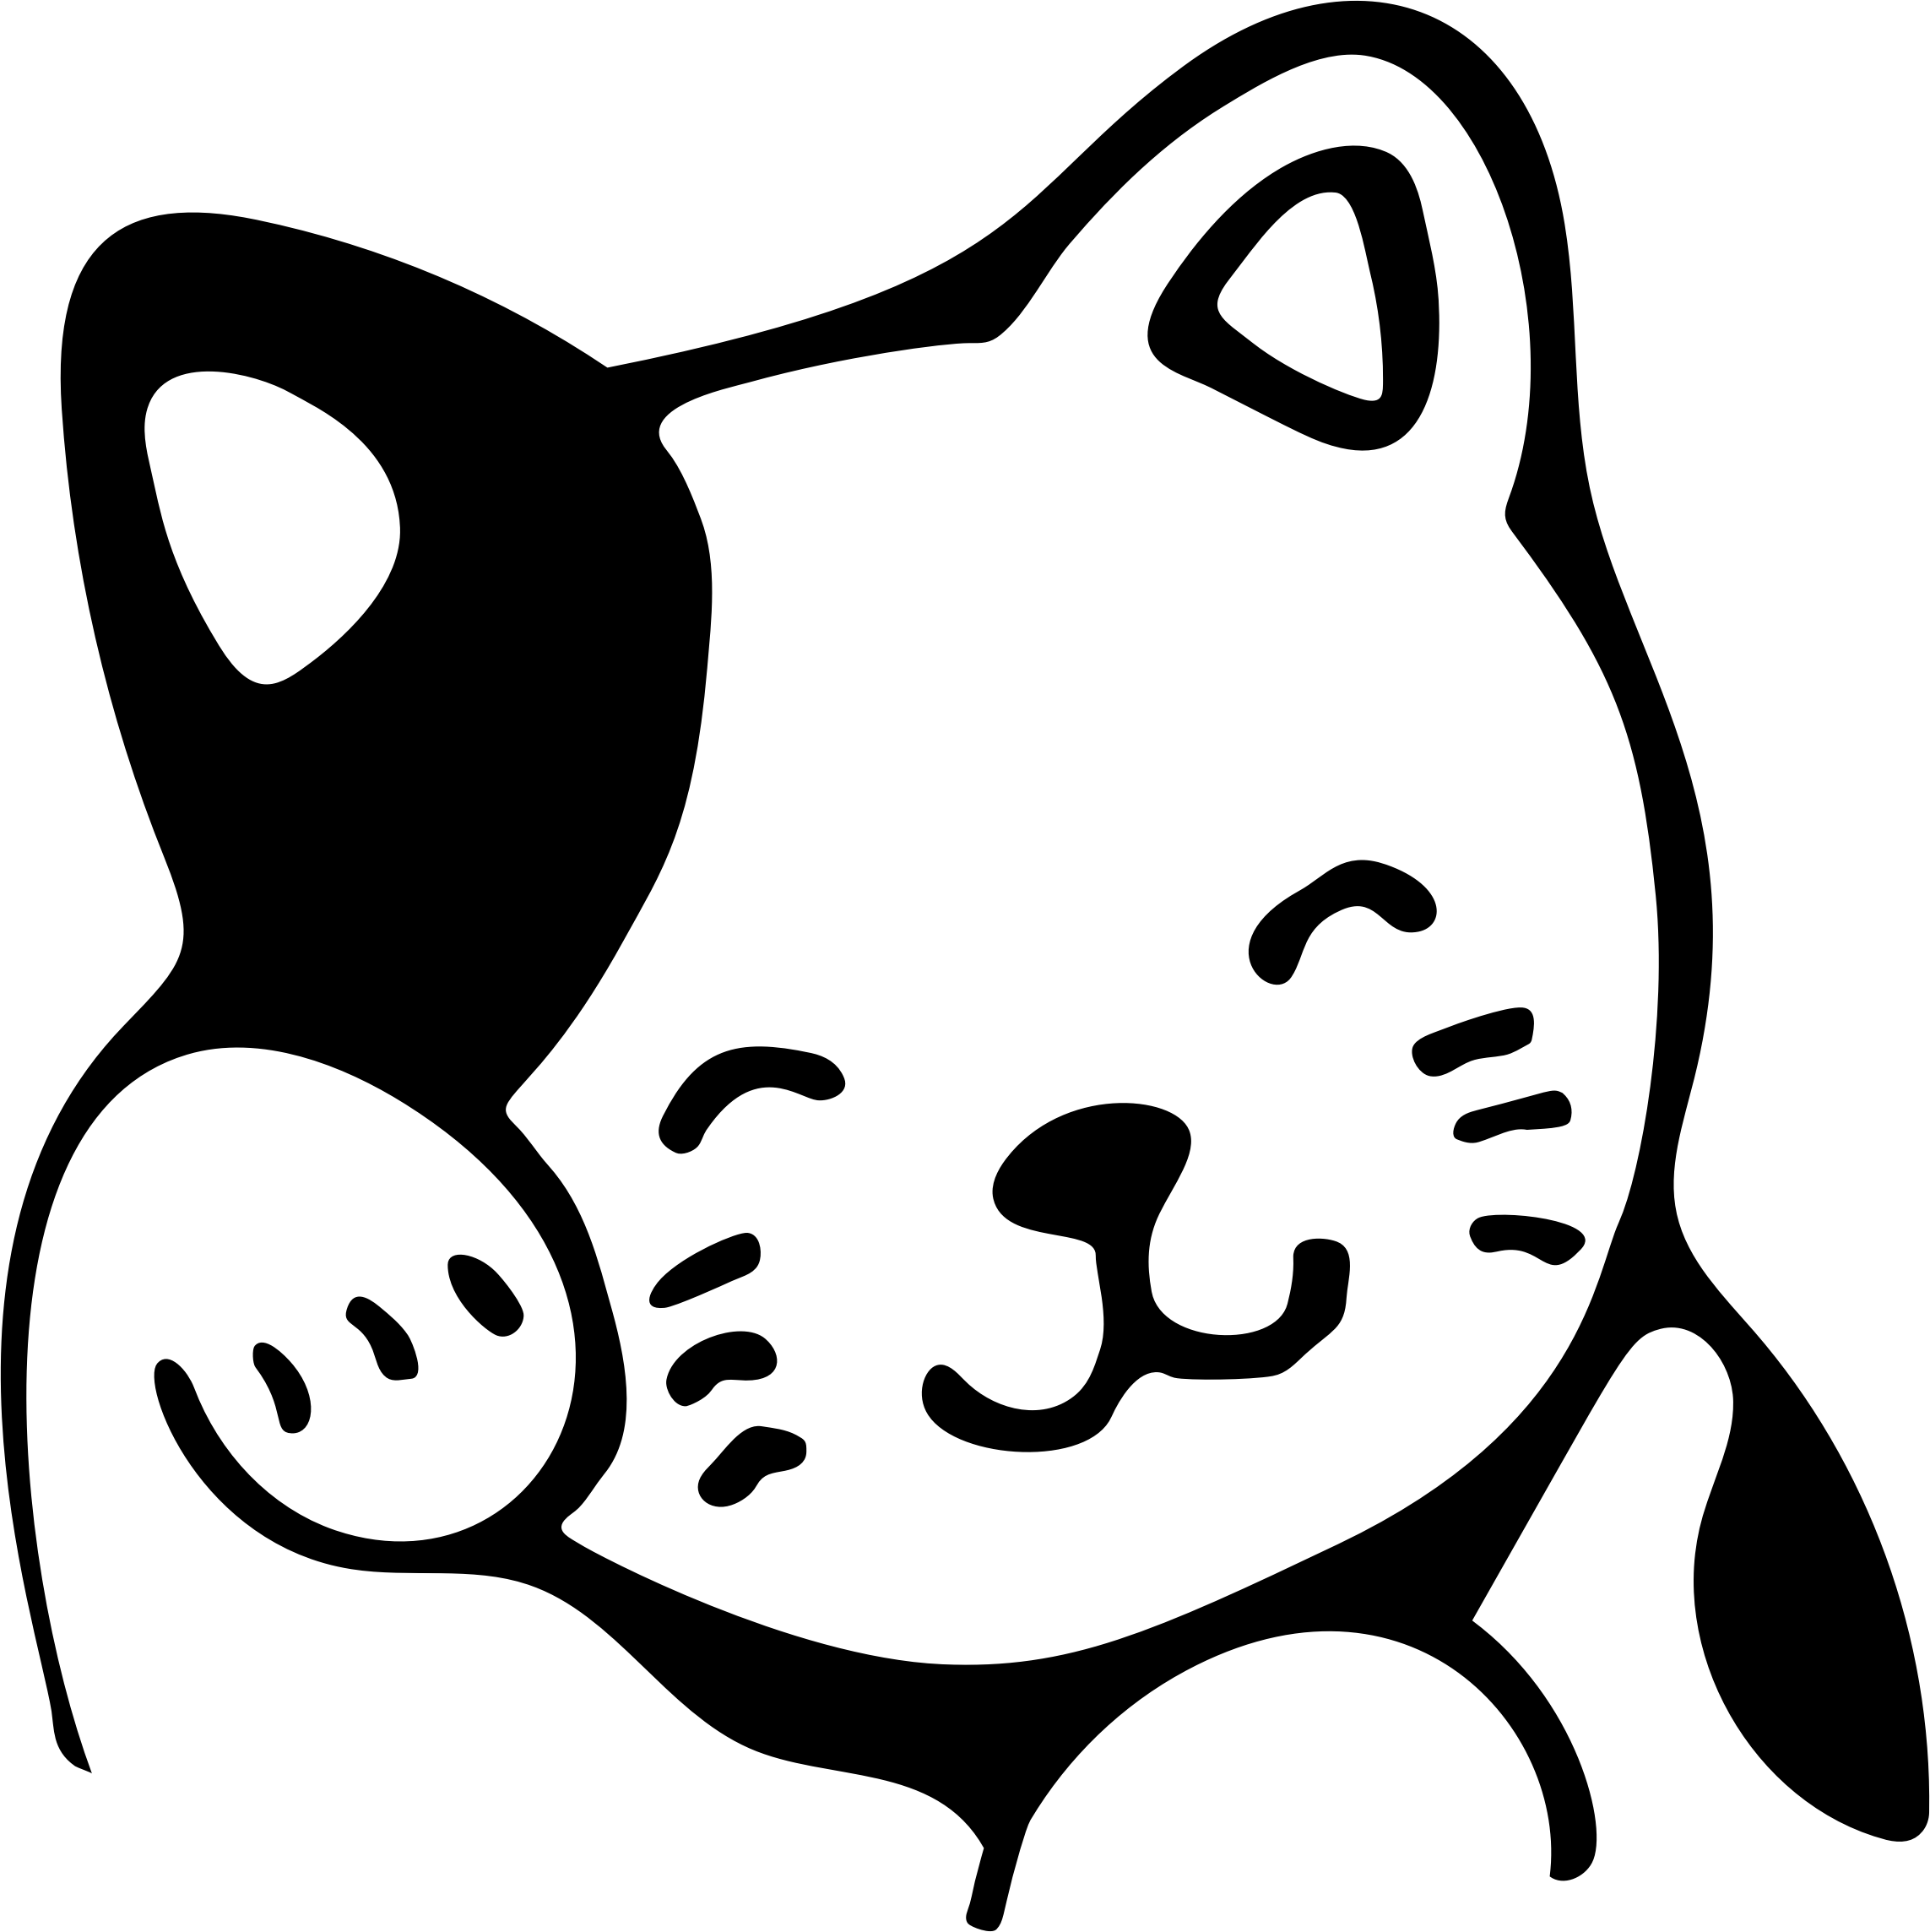
\includegraphics[width=0.3\linewidth]{./misc/happy-cat-grooming-itself-vector-file} 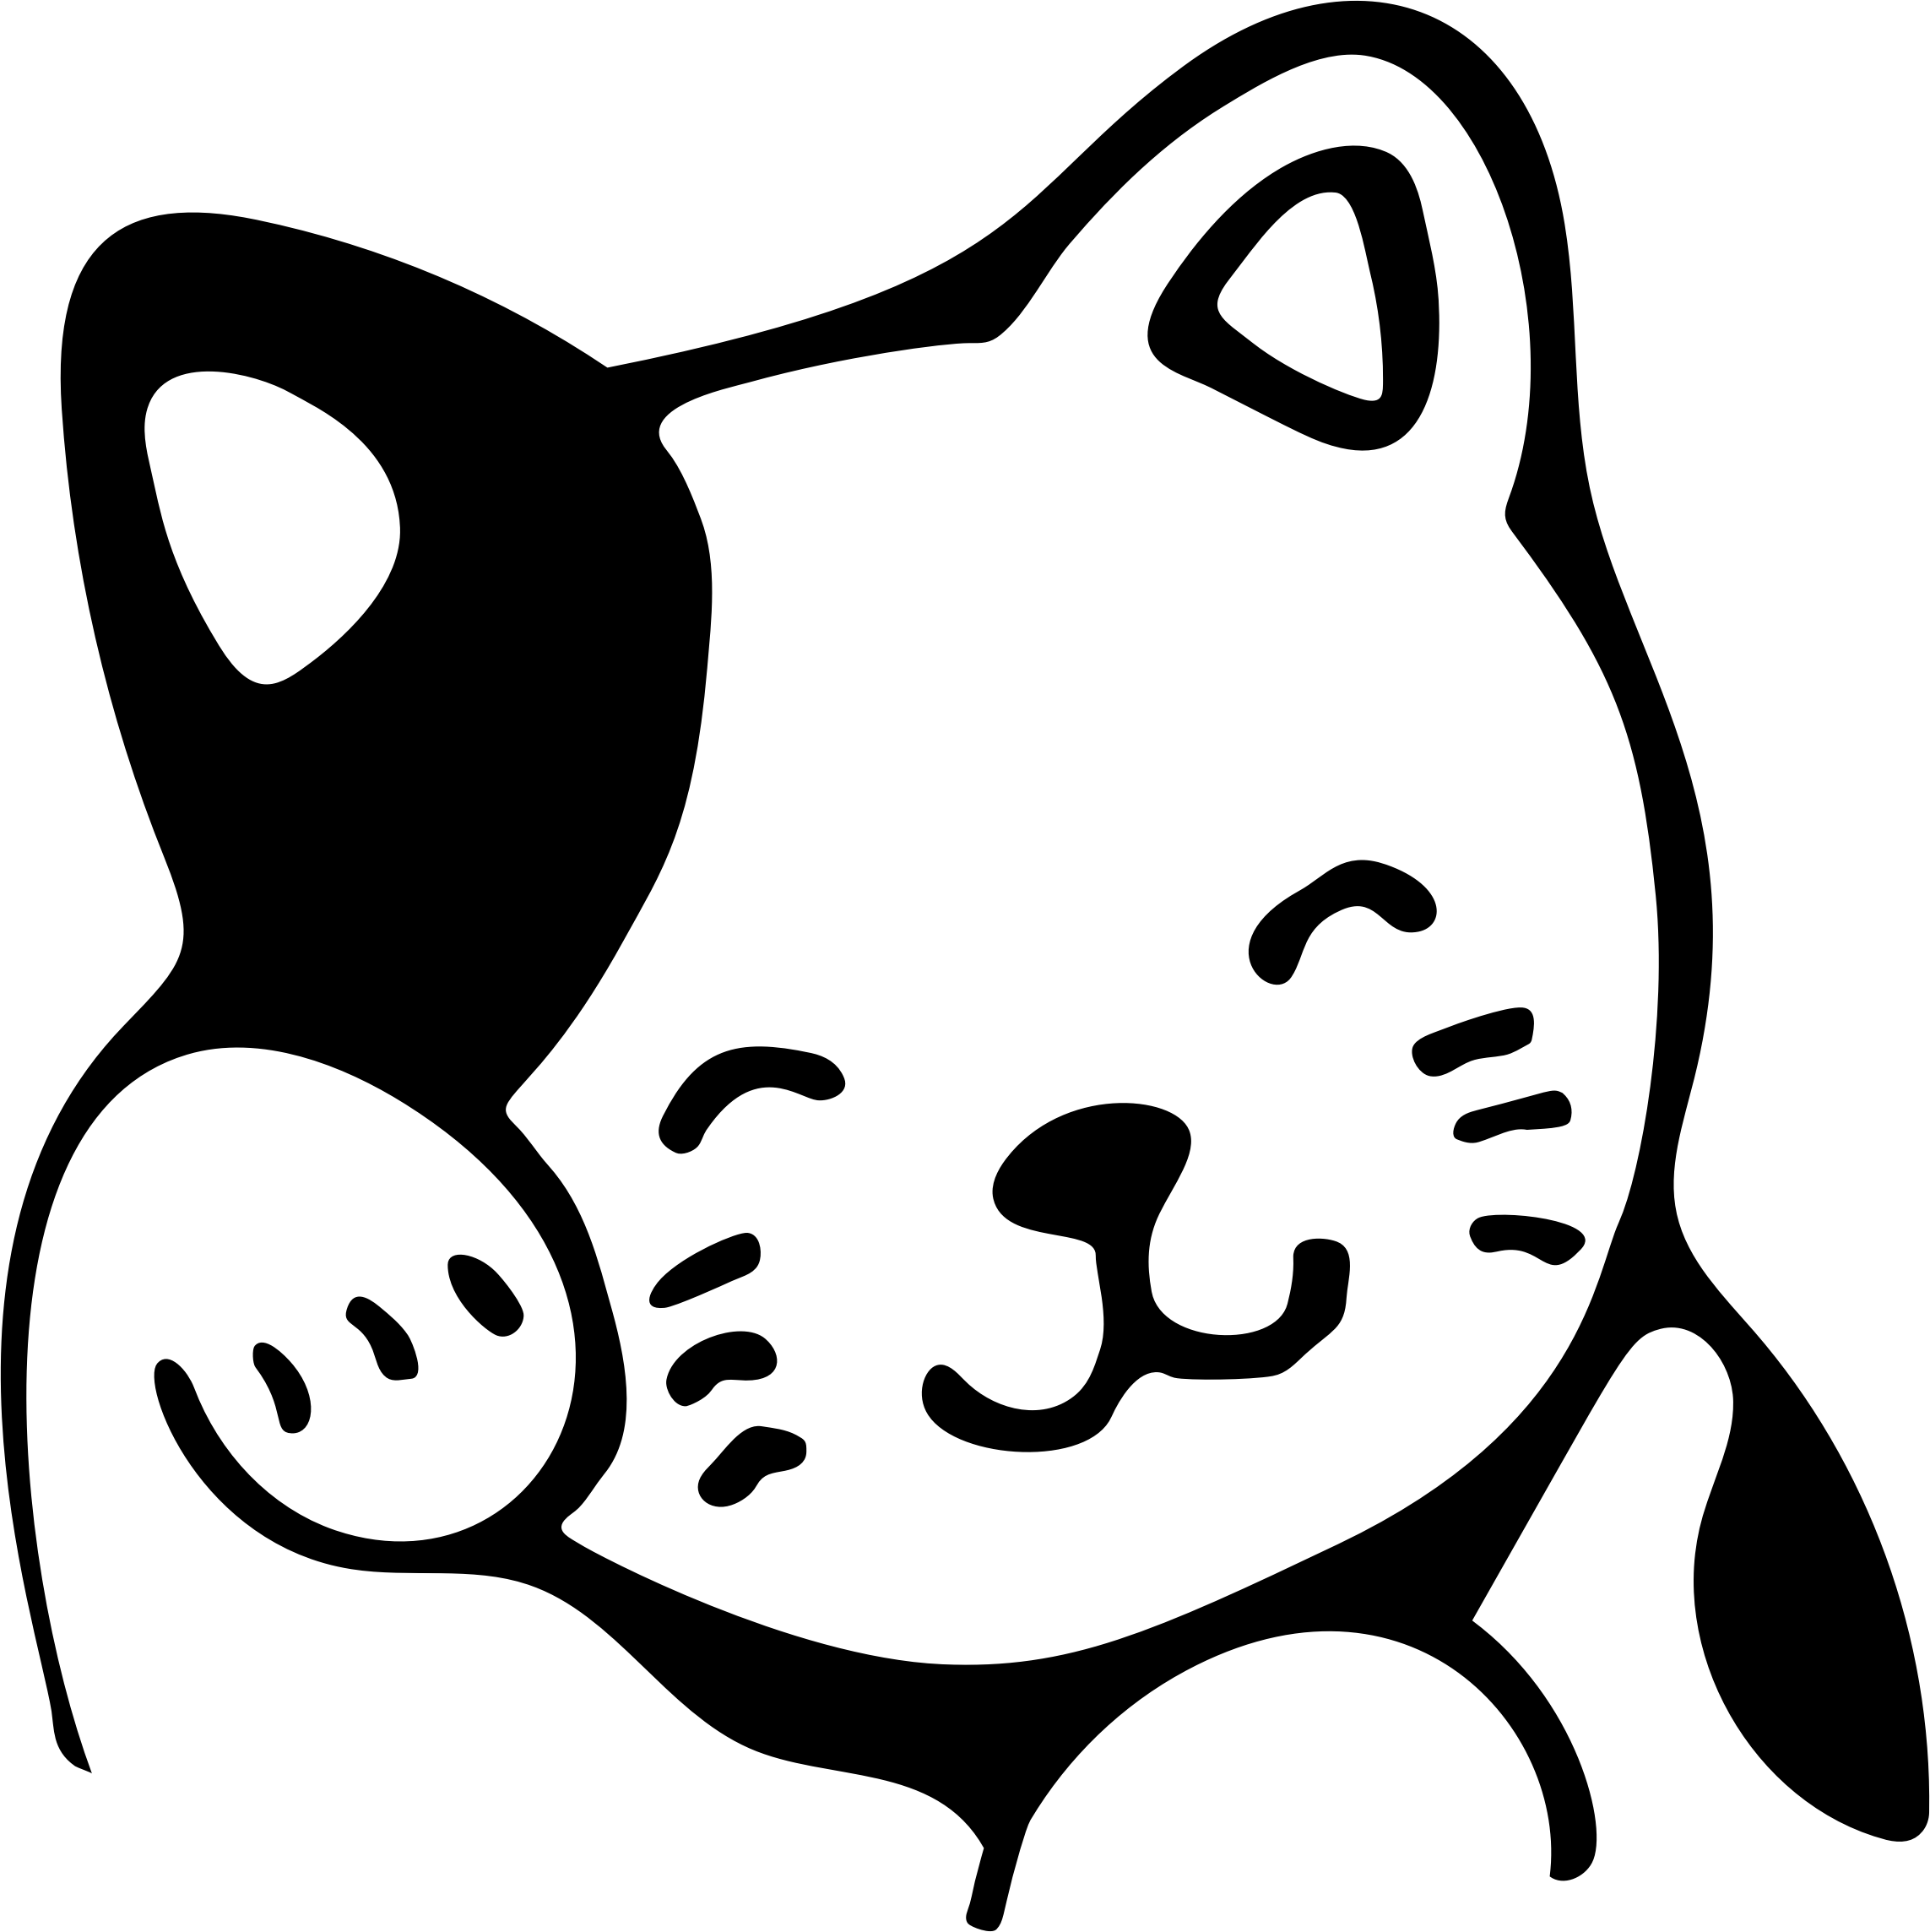
\includegraphics[width=0.3\linewidth]{./misc/happy-cat-grooming-itself-vector-file} \caption{This is a happy cat.}\label{fig:happy-cat}
\end{figure}
\section{Custom blocks}\label{custom-blocks}

\Begin{infobox}

\textbf{Okay}. This book is made with bookdown, an R package/tool-chain
for creating a books in multiple formats. This chapter is just a
placeholder section and some scratch-paper so that I have some examples
on-hand of how to use bookdown's syntax and features.

Some text for this block.
\begin{itemize}
\tightlist
\item
  a list item
\item
  another item
\item
  end the list with a blank line
\end{itemize}
\End{infobox}

\chapter{Quick testing sandbox}\label{quick-testing-sandbox}

\emph{This is a chapter for quickly previewing and testing how content
appears}

We fit a generalized additive model with fast restricted maximum
likelihood estimation {[}Wood (\protect\hyperlink{ref-Wood2017}{2017});
Sóskuthy (\protect\hyperlink{ref-Soskuthy2017}{2017}) for a tutorial for
linguists; see Box 1{]}. We included main effects of study year. These
\emph{parametric} terms work like conventional regression effects and
determined the growth curve's average values. We used age-4 as the
reference year, so the model's intercept represented the average looking
probability at age 4. The model's year effects therefore represented
differences between age 4 vs.~age 3 and age 4 vs.~age 5.

We included a \emph{smooth} term for time. We included a smooth term for
trial time to represent a general effect of time following noun onset
across all studies, and we also included smooth terms for time for each
study. These study-specific smooths estimate how the shape of the data
differs in each individual study. As an equation, our model estimated:
{[}Barr (\protect\hyperlink{ref-Barr2008}{2008});{]} (vers. 2.3; van Rij
et al., \protect\hyperlink{ref-itsadug}{2017})

\Begin{infobox}

\textbf{Box 1: The Intuition Behind Generalized Additive Models}.

In these analyses, the outcome of interest is a value that changes over
time in a nonlinear way. We model these time series by building a set of
features to represent time values. In the growth curve analyses of
familiar word recognition, we used a set of polynomial features which
expressed time as the weighted sum of a linear trend, a quadratic trend
and cubic trend. That is:

\[
\text{log-odds}(\mathit{looking}) = 
  \alpha + \beta_1 * \textit{Time}^1 +
           \beta_2 * \textit{Time}^2 +
           \beta_3 * \textit{Time}^3
\]

But another way to think about the polynomial terms is as \emph{basis
functions}: A set of features that combine to approximate some nonlinear
function of time. Under this framework, the model can be expressed as:

\[
\text{log-odds}(\mathit{looking}) = 
  \alpha + f(\textit{Time})
\]

This is the idea behind generalized additive models and their
\emph{smooth terms}. These smooths fit nonlinear functions of data by
weighting and adding simple functions together. The figures below show 9
basis functions from a ``thin-plate spline'' and how they can be
weighted and summed to fit a growth curve.
\begin{verbatim}
#> Warning: package 'bindrcpp' was built under R version 3.4.4
\end{verbatim}
\begin{center}\includegraphics[width=0.66\linewidth]{81-test_files/figure-latex/infobox-1-figs-1} \end{center}

Each of these basis functions is weighted by a model coefficient, but
the individual basis functions are not a priori meaningful. Rather, it
is the whole set of functions that approximate the curvature of the
data---i.e., \emph{f}(Time))---so we statistically evaluate the whole
batch of coefficients simultaneously. This joint testing is similar to
how one might test a batch of effects in an ANOVA. If the batch of
effects jointly improve model fit, we infer that there is a significant
smooth or shape effect. (Not quite sure this is 100\% accurate yet.)

Smooth terms come with an estimated degrees of freedom (EDF). These
values provide a sense of how many degrees of freedom the smooth
consumed. An EDF of 1 is a perfectly straight line, indicating no
smoothing. Higher EDF values indicate that the smooth term captured more
curvature from the data.

\End{infobox}

\appendix


\chapter{Computational Details for Specific Aim
1}\label{aim1-gca-models}

\section{Growth Curve Analysis
Models}\label{growth-curve-analysis-models}

The models were fit in R (version) with RStanARM (version).

When I computed the orthogonal polynomial features for Time, they were
rescaled so that the linear feature ranged from~−.5 to~.5. Under this
scaling a unit change in Time\textsuperscript{1} was equal to change
from the start to the end of the analysis window. The polynomial
features for the Time had the following ranges:
\begin{tabular}{l|r|r|r}
\hline
Feature & Min & Max & Range\\
\hline
Time\textasciicircum{}1\textasciicircum{} & \&minus;0.50 & 0.50 & 1.00\\
\hline
Time\textasciicircum{}2\textasciicircum{} & \&minus;0.33 & 0.60 & 0.93\\
\hline
Time\textasciicircum{}3\textasciicircum{} & \&minus;0.63 & 0.63 & 1.26\\
\hline
\end{tabular}
Below is the code used to fit the model with RStanARM. It took about
24~hours to run the model. \texttt{ot1}, \texttt{ot2}, and \texttt{ot3}
are the polynomial time features, \texttt{ResearchID} identifies
children, and \texttt{Study} identifies the age/year of the study.
\texttt{Primary} counts the number of looks to the target image at each
time bin; \texttt{Others} counts looks to the other three images.
\begin{Shaded}
\begin{Highlighting}[]
\KeywordTok{library}\NormalTok{(rstanarm)}
\KeywordTok{options}\NormalTok{(}\DataTypeTok{mc.cores =}\NormalTok{ parallel}\OperatorTok{::}\KeywordTok{detectCores}\NormalTok{())}

\NormalTok{m <-}\StringTok{ }\KeywordTok{stan_glmer}\NormalTok{(}
  \KeywordTok{cbind}\NormalTok{(Primary, Others) }\OperatorTok{~}
\StringTok{    }\NormalTok{(ot1 }\OperatorTok{+}\StringTok{ }\NormalTok{ot2 }\OperatorTok{+}\StringTok{ }\NormalTok{ot3) }\OperatorTok{*}\StringTok{ }\NormalTok{Study }\OperatorTok{+}
\StringTok{    }\NormalTok{(ot1 }\OperatorTok{+}\StringTok{ }\NormalTok{ot2 }\OperatorTok{+}\StringTok{ }\NormalTok{ot3 }\OperatorTok{|}\StringTok{ }\NormalTok{ResearchID}\OperatorTok{/}\NormalTok{Study),}
  \DataTypeTok{family =}\NormalTok{ binomial,}
  \DataTypeTok{prior =} \KeywordTok{normal}\NormalTok{(}\DecValTok{0}\NormalTok{, }\DecValTok{1}\NormalTok{, }\DataTypeTok{autoscale =} \OtherTok{FALSE}\NormalTok{),}
  \DataTypeTok{prior_intercept =} \KeywordTok{normal}\NormalTok{(}\DecValTok{0}\NormalTok{, }\DecValTok{2}\NormalTok{),}
  \DataTypeTok{prior_covariance =} \KeywordTok{decov}\NormalTok{(}\DecValTok{2}\NormalTok{, }\DecValTok{1}\NormalTok{, }\DecValTok{1}\NormalTok{),}
  \DataTypeTok{data =}\NormalTok{ d_m)}

\NormalTok{readr}\OperatorTok{::}\KeywordTok{write_rds}\NormalTok{(m, }\StringTok{"./data/stan_aim1_cubic_model.rds.gz"}\NormalTok{)}
\end{Highlighting}
\end{Shaded}
We used moderately informative priors for the main regression effects.
Under the Normal(0~{[}mean{]}, 1~{[}sd{]}) prior, before seeing any
data, we expect 95\%~of plausible effects to fall in the range ±1.96,
which is an adequate range for these growth curve models.

\emph{Here I would have to also describe the random effects structure.}

For the hierarchical part of the model, I used RStanARM's
\texttt{decov()} prior which simultaneously sets a prior of the
variances and correlations of the model's random effect terms.
Practically speaking, variances capture the variation in by-subject and
by-subject-by-age effects, and correlations allow correlations between
the by-subject effects and between the by-subject-by-age effects. For
example, I would expect that participants with average looking
probabilities (low intercepts) to have flatter growth curves (low
Time\textsuperscript{1} effects), and this relationship would be
captured by one of the random-effect correlation terms.

I used the default prior for the variance terms and applied a weakly
informative LKJ(2) prior on the random effect correlations.
Figure~\ref{fig:lkj-prior} shows samples from the prior distribution of
models fit with the default LKJ(1) prior and a weakly informative LKJ(2)
prior. Under LKJ(2), extreme correlations are less plausible. The prior
shifts the probability mass away from the ±1 edges towards the center.
The motivation for this kind of prior was \emph{regularization}: We give
the model a small amount of information to nudge it away from extreme,
degenerate values.



\begin{figure}
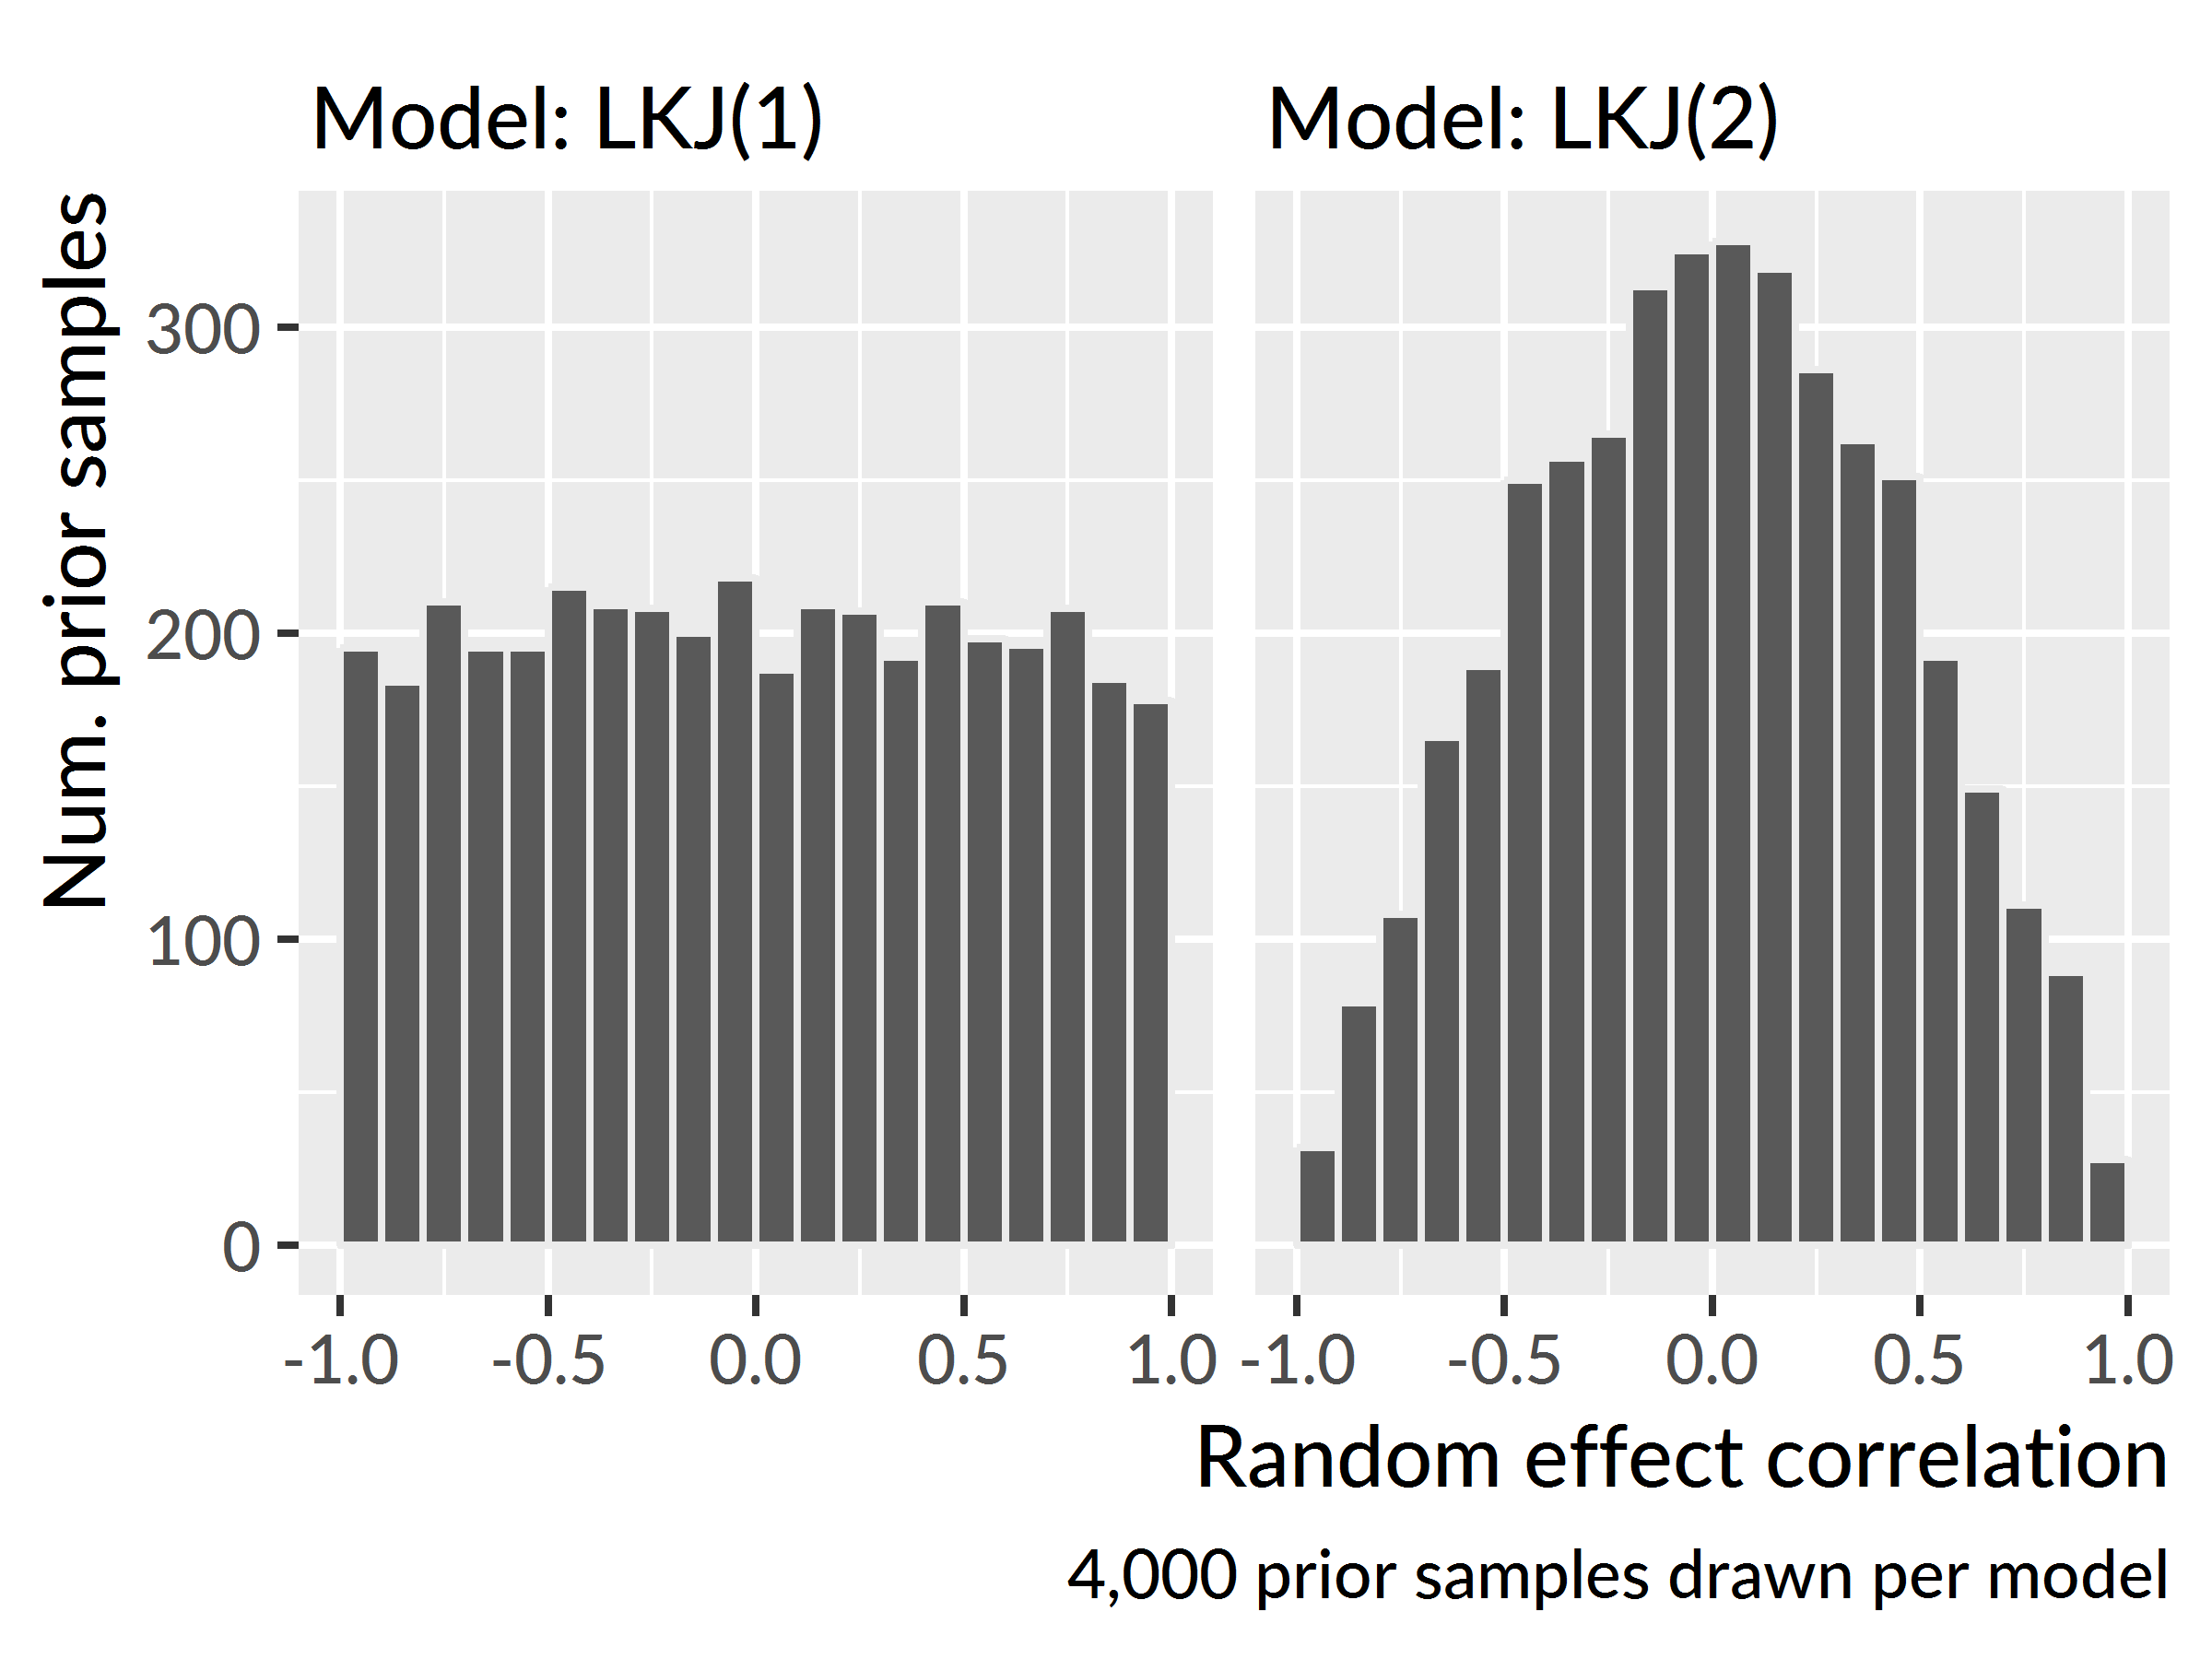
\includegraphics[width=0.5\linewidth]{90-appendix_files/figure-latex/lkj-prior-1} \caption{Samples of correlation effects drawn from the LKJ(1) and
LKJ(2) priors.}\label{fig:lkj-prior}
\end{figure}
\textbf{Box 1: A brief comment about priors.}

Bayesian models require prior information (``priors''). Priors are also
commonly referred to as ``prior beliefs'', and Bayesian techniques are
criticized or dismissed for smuggling subjectivity into the scientific
enterprise. I find this unfortunate on two grounds. First, \emph{belief}
overstates things. As George Box said, ``all models are wrong, but some
are useful'' {[}cite{]}, so no part of a statistical model should be
called a ``belief'' when the whole thing is a convenient fiction. That's
why I prefer the term \emph{prior information}. {[}Hat tip Gelman?{]}
Second, other parts of the statistical model are also subjective:
likelihood functions, what kind of ANOVA, what to covary, whether to
transform measurements, whether a \emph{p}~= .07 is a ``marginal''
effect or no effect at all, and so on. This subjectivity seems
reasonable, provided that we scientists are open about modeling
decisions.

For these models, I will use weakly to moderately informative priors.
For example, suppose \emph{x} and \emph{y} are scaled to mean 0 and
standard deviation 1. A weakly informative prior for the effect of
\emph{x} on \emph{y} might be Normal(0,~5)---a normal distribution with
mean 0 and standard deviation 5. If we fit a regression model and
observed an effect size of 12~SD units, our first assumption would be
that something went wrong with our software. The weakly informative
prior captures this level of prior information. A moderately informative
prior would be Normal(0,~1). This prior information captures our
disciplinary experience that effect sizes greater than ±1 relatively
uncommon in child language research. A strongly informative prior for
this effect might be something like Normal(.4,~.1) which says that our
model should be very skeptical of negative effects and of effects larger
than .8. For this project, I will default to the first two levels of
prior information.

\section{Additional model results}\label{additional-model-results}

The output below contains the model quick view, a summary of the fixed
effect terms, and a summary of the priors used.
\begin{Shaded}
\begin{Highlighting}[]
\NormalTok{b}

\KeywordTok{summary}\NormalTok{(b, }\DataTypeTok{pars =} \KeywordTok{names}\NormalTok{(}\KeywordTok{fixef}\NormalTok{(b)))}

\KeywordTok{prior_summary}\NormalTok{(b)}
\end{Highlighting}
\end{Shaded}
\subsection{Plot the intervals for the random effect
parameters}\label{plot-the-intervals-for-the-random-effect-parameters}

These are the parameters governing the random effect distributions.
First, we plot the standard deviations. Recall that in our hierarchical
model we suppose that each growth curve is drawn from a population of
related curves. The model's fixed effects estimate the means of the
distribution. These terms estimate the variability around that mean. We
did not have any a priori hypotheses about the values of these scales,
so do not discuss them any further.

Then the correlations.

\subsection{Posterior predictive
checks}\label{posterior-predictive-checks}

Bayesian models are generative; they describe how the data could have
been generated. One way to evaluate the model is to have it simulate new
observations. If the simulated data closely resembles the observed data,
then we have some confidence that our model has learned an approximation
of how the data could have been generated. Figure \ref{fig:post-pred}
depicts the density of the observed data from each year of the study
versus 200 posterior simulations. Because the simulations closely track
the density of the observed data, we can infer that the model has
learned how to generate data from each year of the study.














We can ask the model make even more specific posterior predictions.
Below we plot the posterior predictions for random participants. This is
the model simulating new data for these participants.
\begin{Shaded}
\begin{Highlighting}[]
\KeywordTok{set.seed}\NormalTok{(}\DecValTok{09272017}\NormalTok{)}

\NormalTok{ppred <-}\StringTok{ }\NormalTok{d_m }\OperatorTok\StringTok{ }
\StringTok{  }\KeywordTok{sample_n_of}\NormalTok{(}\DecValTok{8}\NormalTok{, ResearchID) }\OperatorTok\StringTok{ }
\StringTok{  }\NormalTok{tristan}\OperatorTok{::}\KeywordTok{augment_posterior_predict}\NormalTok{(b, }\DataTypeTok{newdata =}\NormalTok{ ., }\DataTypeTok{nsamples =} \DecValTok{100}\NormalTok{) }\OperatorTok\StringTok{ }
\StringTok{  }\KeywordTok{mutate}\NormalTok{(}\DataTypeTok{trials =}\NormalTok{ Primary }\OperatorTok{+}\StringTok{ }\NormalTok{Others)}

\KeywordTok{ggplot}\NormalTok{(ppred) }\OperatorTok{+}\StringTok{ }
\StringTok{  }\KeywordTok{aes}\NormalTok{(}\DataTypeTok{x =}\NormalTok{ Time, }\DataTypeTok{y =}\NormalTok{ Prop, }\DataTypeTok{color =}\NormalTok{ Study, }\DataTypeTok{group =}\NormalTok{ Study) }\OperatorTok{+}\StringTok{ }
\StringTok{  }\KeywordTok{geom_line}\NormalTok{(}\KeywordTok{aes}\NormalTok{(}\DataTypeTok{y =}\NormalTok{ .posterior_value }\OperatorTok{/}\StringTok{ }\NormalTok{trials, }
                \DataTypeTok{group =} \KeywordTok{interaction}\NormalTok{(.draw, Study)), }
            \DataTypeTok{alpha =}\NormalTok{ .}\DecValTok{20}\NormalTok{) }\OperatorTok{+}\StringTok{ }
\StringTok{  }\KeywordTok{geom_line}\NormalTok{(}\DataTypeTok{size =} \DecValTok{1}\NormalTok{, }\DataTypeTok{color =} \StringTok{"grey50"}\NormalTok{) }\OperatorTok{+}\StringTok{ }
\StringTok{  }\KeywordTok{facet_wrap}\NormalTok{(}\StringTok{"ResearchID"}\NormalTok{) }\OperatorTok{+}\StringTok{ }
\StringTok{  }\KeywordTok{theme}\NormalTok{(}
    \DataTypeTok{legend.position =} \KeywordTok{c}\NormalTok{(.}\DecValTok{95}\NormalTok{, }\DecValTok{0}\NormalTok{), }
    \DataTypeTok{legend.justification =} \KeywordTok{c}\NormalTok{(}\DecValTok{1}\NormalTok{, }\DecValTok{0}\NormalTok{),}
    \DataTypeTok{legend.margin =} \KeywordTok{margin}\NormalTok{(}\DecValTok{0}\NormalTok{)) }\OperatorTok{+}
\StringTok{  }\KeywordTok{guides}\NormalTok{(}\DataTypeTok{color =} \KeywordTok{guide_legend}\NormalTok{(}\DataTypeTok{title =} \OtherTok{NULL}\NormalTok{, }\DataTypeTok{override.aes =} \KeywordTok{list}\NormalTok{(}\DataTypeTok{alpha =} \DecValTok{1}\NormalTok{))) }\OperatorTok{+}
\StringTok{  }\KeywordTok{labs}\NormalTok{(}
    \DataTypeTok{title =} \StringTok{"Observed means and 100 simulations of new data"}\NormalTok{,}
    \DataTypeTok{x =} \StringTok{"Time after target onset [ms]"}\NormalTok{,}
    \DataTypeTok{y =} \StringTok{"Proportion looks to target"}\NormalTok{) }
\end{Highlighting}
\end{Shaded}
Or we can plot the linear predictions. These are posterior predictions
of the log-odds of looking to target before adding binomial noise.
\begin{Shaded}
\begin{Highlighting}[]
\NormalTok{lpred <-}\StringTok{ }\NormalTok{d_m }\OperatorTok\StringTok{ }
\StringTok{  }\KeywordTok{sample_n_of}\NormalTok{(}\DecValTok{8}\NormalTok{, ResearchID) }\OperatorTok\StringTok{ }
\StringTok{  }\NormalTok{tristan}\OperatorTok{::}\KeywordTok{augment_posterior_linpred}\NormalTok{(b, }\DataTypeTok{newdata =}\NormalTok{ ., }\DataTypeTok{nsamples =} \DecValTok{100}\NormalTok{)}

\KeywordTok{ggplot}\NormalTok{(lpred) }\OperatorTok{+}\StringTok{ }
\StringTok{  }\KeywordTok{aes}\NormalTok{(}\DataTypeTok{x =}\NormalTok{ Time, }\DataTypeTok{y =}\NormalTok{ .posterior_value, }\DataTypeTok{color =}\NormalTok{ Study) }\OperatorTok{+}
\StringTok{  }\KeywordTok{geom_line}\NormalTok{(}\KeywordTok{aes}\NormalTok{(}\DataTypeTok{group =} \KeywordTok{interaction}\NormalTok{(Study, ResearchID, .draw)), }
            \DataTypeTok{alpha =}\NormalTok{ .}\DecValTok{1}\NormalTok{) }\OperatorTok{+}
\StringTok{  }\KeywordTok{facet_wrap}\NormalTok{(}\StringTok{"ResearchID"}\NormalTok{) }\OperatorTok{+}\StringTok{ }
\StringTok{  }\KeywordTok{geom_point}\NormalTok{(}\KeywordTok{aes}\NormalTok{(}\DataTypeTok{y =} \KeywordTok{qlogis}\NormalTok{(Prop)), }\DataTypeTok{shape =} \DecValTok{1}\NormalTok{) }\OperatorTok{+}\StringTok{ }
\StringTok{  }\KeywordTok{theme}\NormalTok{(}
    \DataTypeTok{legend.position =} \KeywordTok{c}\NormalTok{(.}\DecValTok{95}\NormalTok{, }\DecValTok{0}\NormalTok{), }
    \DataTypeTok{legend.justification =} \KeywordTok{c}\NormalTok{(}\DecValTok{1}\NormalTok{, }\DecValTok{0}\NormalTok{),}
    \DataTypeTok{legend.margin =} \KeywordTok{margin}\NormalTok{(}\DecValTok{0}\NormalTok{)) }\OperatorTok{+}
\StringTok{  }\KeywordTok{guides}\NormalTok{(}\DataTypeTok{color =} \KeywordTok{guide_legend}\NormalTok{(}\DataTypeTok{title =} \OtherTok{NULL}\NormalTok{, }\DataTypeTok{override.aes =} \KeywordTok{list}\NormalTok{(}\DataTypeTok{alpha =} \DecValTok{1}\NormalTok{))) }\OperatorTok{+}
\StringTok{  }\KeywordTok{labs}\NormalTok{(}
    \DataTypeTok{title =} \StringTok{"Observed data and 100 posterior predictions"}\NormalTok{,}
    \DataTypeTok{x =} \StringTok{"Time after target onset [ms]"}\NormalTok{,}
    \DataTypeTok{y =} \StringTok{"Posterior log-odds"}\NormalTok{)}
\end{Highlighting}
\end{Shaded}
\hypertarget{vw-experiment-items}{\chapter{Items used in the visual
world experiment}\label{vw-experiment-items}}

Each row of the table represents a set of four images used in a trial
for the experiment. There were two blocks of trials with different
images and trial orderings. For the two unrelated foils with more than
one word listed, the first word was used in block one and the second in
block two.
\begin{longtable}[]{@{}llll@{}}
\toprule
\textbf{Target} & \textbf{Phonological} & \textbf{Semantic} &
\textbf{Unrelated}\tabularnewline
\midrule
\endhead
bear & bell & horse & ring\tabularnewline
bee & bear & fly & heart\tabularnewline
bell & bee & drum & swing\tabularnewline
bread & bear & cheese & vase\tabularnewline
cheese & shirt & bread & van\tabularnewline
dress & drum & shirt & swing\tabularnewline
drum & dress & bell & sword\tabularnewline
flag & fly & kite & pear\tabularnewline
fly & flag & bee & pen\tabularnewline
gift & kite & vase & bread\tabularnewline
heart & horse & ring & bread/pan\tabularnewline
horse & heart & bear & pan\tabularnewline
kite & gift & flag & shirt\tabularnewline
pan & pear & spoon & vase\tabularnewline
pear & pen & cheese & ring/vase\tabularnewline
pen & pear & sword & van\tabularnewline
ring & swing & dress & flag\tabularnewline
shirt & cheese & dress & fly\tabularnewline
spoon & swan & pan & drum\tabularnewline
swan & spoon & bee & bell\tabularnewline
swing & spoon & kite & heart\tabularnewline
sword & swan & pen & gift\tabularnewline
van & pan & horse & sword\tabularnewline
vase & van & gift & swan\tabularnewline
\bottomrule
\end{longtable}
\hypertarget{mp-experiment-items}{\chapter{Items used in the
mispronunciation experiment}\label{mp-experiment-items}}

The stimuli changed between Year~1 and Year 2 so that dog/tog was
replaced with rice/wice.
\begin{longtable}[]{@{}llllll@{}}
\toprule
\textbf{Time Points} & \textbf{Word Group} & \textbf{Condition} &
\textbf{Audio (IPA)} & \textbf{Familiar Object} & \textbf{Unfamiliar
Object}\tabularnewline
\midrule
\endhead
1 & dog & Correct Production & /dɔg/ & dog & wombat\tabularnewline
& & Mispronunciation & /tɔg/ & dog & wombat\tabularnewline
& & Nonword & /vef/ & ball & sextant\tabularnewline
1, 2, 3 & cake & Correct Production & /kek/ & cake & horned
melon\tabularnewline
& & Mispronunciation & /gek/ & cake & horned melon\tabularnewline
& & Nonword & /pʌm/ & book & churn\tabularnewline
1, 2, 3 & duck & Correct Production & /dʌk/ & duck & toy
creature\tabularnewline
& & Mispronunciation & /gʌk/ & duck & toy creature\tabularnewline
& & Nonword & /ʃæn/ & cup & reed\tabularnewline
1, 2, 3 & girl & Correct Production & /gɜ˞l/ & girl &
marmoset\tabularnewline
& & Mispronunciation & /dɜ˞l/ & girl & marmoset\tabularnewline
& & Nonword & /nedʒ/ & car & work holder\tabularnewline
1, 2, 3 & shoes & Correct Production & /ʃuz/ & shoes &
flasks\tabularnewline
& & Mispronunciation & /suz/ & shoes & flasks\tabularnewline
& & Nonword & /giv/ & sock & trolley\tabularnewline
1, 2, 3 & soup & Correct Production & /sup/ & soup &
steamer\tabularnewline
& & Mispronunciation & /ʃup/ & soup & steamer\tabularnewline
& & Nonword & /tʃim/ & bed & pastry mixer\tabularnewline
2, 3 & rice & Correct Production & /ɹaɪs/ & rice & anise\tabularnewline
& & Mispronunciation & /waɪs/ & rice & anise\tabularnewline
& & Nonword & /bep/ & ball & sextant\tabularnewline
\bottomrule
\end{longtable}
\chapter{Related Work}\label{related-work}

In this section, I clarify relationships between this project and other
word recognition research reported from our lab. In short, our lab has
reported results about the two-image and four-image experiments from
cross-sectional samples, describing child-level measures that predict
performance in these tasks. In contrast, my dissertation 1) focuses on
the longitudinal development of word recognition and 2) engages with the
fine-grained details of lexical processing.

Law \& Edwards (\protect\hyperlink{ref-MPPaper}{2015}) analyzed a
different version of the mispronunciation experiment on a different
sample of children (\emph{n}~= 34, 30-46 months old). This earlier
version included both real word and the mispronunciation of the real
word in the same block of trial. For example, a child would hear ``dog''
and ``tog'' during the same session of the experiment. This design might
subtly temper the effect of mispronounced stimuli by allowing the
listener to compare the mispronunciation to its correctly produced
counterpart. The version of the experiment in Specific Aim~2 separates
the real words and mispronunciations so that a child never hears a
familiar word and its mispronunciation during the same block of trials.
With this design, there is no explicit point of comparison for the
mispronunciation, and the child has to rely on his or her own lexical
representations when processing these words.

Law et al. (\protect\hyperlink{ref-RWLPaper}{2016}) analyzed data from
the four-image experiment in Specific Aim~1. This study featured a
diverse cross-sectional sample of 60 children, half of whom received the
experiment in African American English and half received it in
Mainstream American English. The sample ranged in age from~28 to~60
months. The study ``borrowed'' data from~23 participants from Year~1 of
the longitudinal study to enrich parts of the samples demographics. For
this manuscript, we analyzed how vocabulary and maternal education
predicted looking patterns, including relative looks to the semantic and
phonological foils.

Mahr and Edwards (in press) was the manuscript I originally authored for
my preliminary examinations. The paper analyzes the same kinds of
relations as Weisleder \& Fernald
(\protect\hyperlink{ref-Weisleder2013}{2013}) which showed that lexical
processing efficiency mediated the effect of language input on future
vocabulary size. In particular, I asked whether word recognition
performance on the four-image task of Specific Aim~1, vocabulary size,
and home language input data from Year~1 predicted vocabulary size at
Year~2. The paper only examined looks to the familiar image from one
year of the study, so it did not analyze any lexical competition effects
or the development of word recognition within children.

\backmatter

\chapter*{Colophon}\label{colophon}
\addcontentsline{toc}{chapter}{Colophon}

\section{Debug info}\label{debug-info}
\begin{Shaded}
\begin{Highlighting}[]
\KeywordTok{str}\NormalTok{(}\KeywordTok{list}\NormalTok{(}\DataTypeTok{html =} \KeywordTok{is_html_output}\NormalTok{(), }\DataTypeTok{latex =} \KeywordTok{is_latex_output}\NormalTok{(),}
         \DataTypeTok{word =} \KeywordTok{is_word_output}\NormalTok{(), }\DataTypeTok{width =} \KeywordTok{options}\NormalTok{(}\StringTok{"width"}\NormalTok{)[[}\DecValTok{1}\NormalTok{]]))}
\CommentTok{#> List of 4}
\CommentTok{#>  $ html : logi FALSE}
\CommentTok{#>  $ latex: logi TRUE}
\CommentTok{#>  $ word : logi FALSE}
\CommentTok{#>  $ width: int 80}

\NormalTok{devtools}\OperatorTok{::}\KeywordTok{session_info}\NormalTok{()}
\CommentTok{#> Session info ------------------------------------------------------------------}
\CommentTok{#>  setting  value                       }
\CommentTok{#>  version  R version 3.4.3 (2017-11-30)}
\CommentTok{#>  system   x86_64, mingw32             }
\CommentTok{#>  ui       RTerm                       }
\CommentTok{#>  language (EN)                        }
\CommentTok{#>  collate  English_United States.1252  }
\CommentTok{#>  tz       America/Chicago             }
\CommentTok{#>  date     2018-04-13}
\CommentTok{#> Packages ----------------------------------------------------------------------}
\CommentTok{#>  package    * version date       source        }
\CommentTok{#>  assertthat   0.2.0   2017-04-11 CRAN (R 3.3.2)}
\CommentTok{#>  backports    1.1.2   2017-12-13 CRAN (R 3.4.3)}
\CommentTok{#>  base       * 3.4.3   2017-11-30 local         }
\CommentTok{#>  bindr        0.1.1   2018-03-13 CRAN (R 3.4.3)}
\CommentTok{#>  bindrcpp     0.2.2   2018-03-29 CRAN (R 3.4.4)}
\CommentTok{#>  bookdown     0.7     2018-02-18 CRAN (R 3.4.3)}
\CommentTok{#>  colorspace   1.3-2   2016-12-14 CRAN (R 3.3.2)}
\CommentTok{#>  compiler     3.4.3   2017-11-30 local         }
\CommentTok{#>  datasets   * 3.4.3   2017-11-30 local         }
\CommentTok{#>  devtools     1.13.5  2018-02-18 CRAN (R 3.4.3)}
\CommentTok{#>  digest       0.6.15  2018-01-28 CRAN (R 3.4.3)}
\CommentTok{#>  dplyr        0.7.4   2017-09-28 CRAN (R 3.4.2)}
\CommentTok{#>  evaluate     0.10.1  2017-06-24 CRAN (R 3.4.1)}
\CommentTok{#>  ggplot2      2.2.1   2016-12-30 CRAN (R 3.4.1)}
\CommentTok{#>  glue         1.2.0   2017-10-29 CRAN (R 3.4.2)}
\CommentTok{#>  graphics   * 3.4.3   2017-11-30 local         }
\CommentTok{#>  grDevices  * 3.4.3   2017-11-30 local         }
\CommentTok{#>  grid         3.4.3   2017-11-30 local         }
\CommentTok{#>  gtable       0.2.0   2016-02-26 CRAN (R 3.2.3)}
\CommentTok{#>  htmltools    0.3.6   2017-04-28 CRAN (R 3.4.0)}
\CommentTok{#>  huskydown    0.0.4   2018-04-13 local         }
\CommentTok{#>  knitr        1.20    2018-02-20 CRAN (R 3.4.3)}
\CommentTok{#>  lazyeval     0.2.1   2017-10-29 CRAN (R 3.4.2)}
\CommentTok{#>  magrittr     1.5     2014-11-22 CRAN (R 3.1.2)}
\CommentTok{#>  memoise      1.1.0   2017-04-21 CRAN (R 3.3.2)}
\CommentTok{#>  methods    * 3.4.3   2017-11-30 local         }
\CommentTok{#>  munsell      0.4.3   2016-02-13 CRAN (R 3.2.3)}
\CommentTok{#>  parallel     3.4.3   2017-11-30 local         }
\CommentTok{#>  pillar       1.2.1   2018-02-27 CRAN (R 3.4.3)}
\CommentTok{#>  pkgconfig    2.0.1   2017-03-21 CRAN (R 3.3.3)}
\CommentTok{#>  plyr         1.8.4   2016-06-08 CRAN (R 3.3.0)}
\CommentTok{#>  R6           2.2.2   2017-06-17 CRAN (R 3.4.0)}
\CommentTok{#>  Rcpp         0.12.16 2018-03-13 CRAN (R 3.4.4)}
\CommentTok{#>  rlang        0.2.0   2018-02-20 CRAN (R 3.4.3)}
\CommentTok{#>  rmarkdown    1.9     2018-03-01 CRAN (R 3.4.3)}
\CommentTok{#>  rprojroot    1.3-2   2018-01-03 CRAN (R 3.4.3)}
\CommentTok{#>  scales       0.5.0   2017-08-24 CRAN (R 3.4.1)}
\CommentTok{#>  stats      * 3.4.3   2017-11-30 local         }
\CommentTok{#>  stringi      1.1.7   2018-03-12 CRAN (R 3.4.4)}
\CommentTok{#>  stringr      1.3.0   2018-02-19 CRAN (R 3.4.3)}
\CommentTok{#>  tibble       1.4.2   2018-01-22 CRAN (R 3.4.3)}
\CommentTok{#>  tools        3.4.3   2017-11-30 local         }
\CommentTok{#>  utils      * 3.4.3   2017-11-30 local         }
\CommentTok{#>  withr        2.1.2   2018-03-15 CRAN (R 3.4.4)}
\CommentTok{#>  xfun         0.1     2018-01-22 CRAN (R 3.4.3)}
\CommentTok{#>  yaml         2.1.18  2018-03-08 CRAN (R 3.4.3)}

\NormalTok{last_four_commits <-}\StringTok{ }\NormalTok{git2r}\OperatorTok{::}\KeywordTok{commits}\NormalTok{(git2r}\OperatorTok{::}\KeywordTok{repository}\NormalTok{(}\StringTok{"."}\NormalTok{), }\DataTypeTok{n =} \DecValTok{4}\NormalTok{)}
\NormalTok{msgs <-}\StringTok{ }\KeywordTok{lapply}\NormalTok{(last_four_commits, methods}\OperatorTok{::}\NormalTok{show)}
\CommentTok{#> [348d182] 2018-04-13: rename aim1 chapter files}
\CommentTok{#> [e90d795] 2018-04-12: work on discussion}
\CommentTok{#> [7b11b40] 2018-04-12: start general discussion}
\CommentTok{#> [d951535] 2018-04-12: packages updated}
\end{Highlighting}
\end{Shaded}
Built with love using R (Version 3.4.3; R Core Team,
\protect\hyperlink{ref-R-base}{2017}) and the R-packages
\emph{bayesplot} (Version 1.5.0; Gabry \& Mahr,
\protect\hyperlink{ref-R-bayesplot}{2018}), \emph{bookdown} (Version
0.7; Xie,
\protect\hyperlink{ref-R-bookdown}{2018}\protect\hyperlink{ref-R-bookdown}{a}),
\emph{dplyr} (Version 0.7.4; Wickham, Francois, Henry, \& Müller,
\protect\hyperlink{ref-R-dplyr}{2017}), \emph{ggplot2} (Version 2.2.1;
Wickham \& Chang, \protect\hyperlink{ref-R-ggplot2}{2016}), \emph{knitr}
(Version 1.20; Xie,
\protect\hyperlink{ref-R-knitr}{2018}\protect\hyperlink{ref-R-knitr}{b}),
\emph{littlelisteners} (Version 0.0.0.9000; Tristan Mahr,
\protect\hyperlink{ref-R-littlelisteners}{2018}), \emph{lme4} (Version
1.1.17; Bates, Maechler, Bolker, \& Walker,
\protect\hyperlink{ref-R-lme4}{2018}), \emph{rlang} (Version 0.2.0;
Henry \& Wickham, \protect\hyperlink{ref-R-rlang}{2018}),
\emph{rmarkdown} (Version 1.9; Allaire et al.,
\protect\hyperlink{ref-R-rmarkdown}{2018}), \emph{rstanarm} (Version
2.17.3; Gabry \& Goodrich, \protect\hyperlink{ref-R-rstanarm}{2018}),
\emph{tjmisc} (Version 0.0.0.9000; TJ Mahr,
\protect\hyperlink{ref-R-tjmisc}{2018}\protect\hyperlink{ref-R-tjmisc}{a}),
and \emph{tristan} (Version 0.0.0.9000; TJ Mahr,
\protect\hyperlink{ref-R-tristan}{2018}\protect\hyperlink{ref-R-tristan}{b}).
\begin{center}\rule{0.5\linewidth}{\linethickness}\end{center}

This is the original colophon from the huskydown package. I need to
reword and note my modifications.
\begin{quote}
This document is set in \href{https://github.com/georgd/EB-Garamond}{EB
Garamond}, \href{https://github.com/adobe-fonts/source-code-pro/}{Source
Code Pro} and \href{http://www.latofonts.com/lato-free-fonts/}{Lato}.
The body text is set at 11pt with \(\familydefault\).
\end{quote}
\begin{quote}
It was written in R Markdown and \(\LaTeX\), and rendered into PDF using
\href{https://github.com/benmarwick/huskydown}{huskydown} and
\href{https://github.com/rstudio/bookdown}{bookdown}.
\end{quote}
\begin{quote}
This document was typeset using the XeTeX typesetting system, and the
\href{http://staff.washington.edu/fox/tex/}{University of Washington
Thesis class} class created by Jim Fox. Under the hood, the
\href{https://github.com/UWIT-IAM/UWThesis}{University of Washington
Thesis LaTeX template} is used to ensure that documents conform
precisely to submission standards. Other elements of the document
formatting source code have been taken from the
\href{https://github.com/stevenpollack/ucbthesis}{Latex, Knitr, and
RMarkdown templates for UC Berkeley's graduate thesis}, and
\href{https://github.com/suchow/Dissertate}{Dissertate: a LaTeX
dissertation template to support the production and typesetting of a PhD
dissertation at Harvard, Princeton, and NYU}
\end{quote}
\begin{quote}
The source files for this thesis, along with all the data files, have
been organised into an R package, xxx, which is available at
\url{https://github.com/xxx/xxx}. A hard copy of the thesis can be found
in the University of Washington library.
\end{quote}
\backmatter

\chapter*{References}\label{references}
\addcontentsline{toc}{chapter}{References}

\markboth{References}{References}

\hypertarget{refs}{}
\hypertarget{ref-R-rmarkdown}{}
Allaire, J., Xie, Y., McPherson, J., Luraschi, J., Ushey, K., Atkins,
A., \ldots{} Chang, W. (2018). \emph{Rmarkdown: Dynamic documents for
r}. Retrieved from \url{https://CRAN.R-project.org/package=rmarkdown}

\hypertarget{ref-Barr2008}{}
Barr, D. J. (2008). Analyzing `visual world' eyetracking data using
multilevel logistic regression. \emph{Journal of Memory and Language},
\emph{59}(4), 457--474.
doi:\href{https://doi.org/10.1016/j.jml.2007.09.002}{10.1016/j.jml.2007.09.002}

\hypertarget{ref-R-lme4}{}
Bates, D., Maechler, M., Bolker, B., \& Walker, S. (2018). \emph{Lme4:
Linear mixed-effects models using 'eigen' and s4}. Retrieved from
\url{https://CRAN.R-project.org/package=lme4}

\hypertarget{ref-Cristia2014_Review}{}
Cristia, A., Seidl, A., Junge, C., Soderstrom, M., \& Hagoort, P.
(2014). Predicting individual variation in language from infant speech
perception measures. \emph{Child Development}, \emph{85}(4), 1330--1345.
doi:\href{https://doi.org/10.1111/cdev.12193}{10.1111/cdev.12193}

\hypertarget{ref-EllisWeismer2016}{}
Ellis Weismer, S., Haebig, E., Edwards, J. R., Saffran, J. R., \&
Venker, C. E. (2016). Lexical processing in toddlers with ASD: Does weak
central coherence play a role? \emph{Journal of Autism and Developmental
Disorders}, \emph{46}(12), 3755--3769.
doi:\href{https://doi.org/10.1007/s10803-016-2926-y}{10.1007/s10803-016-2926-y}

\hypertarget{ref-Fernald2012}{}
Fernald, A., \& Marchman, V. A. (2012). Individual differences in
lexical processing at 18 months predict vocabulary growth in typically
developing and late-talking toddlers. \emph{Child Development},
\emph{83}(1), 203--222.
doi:\href{https://doi.org/10.1111/j.1467-8624.2011.01692.x}{10.1111/j.1467-8624.2011.01692.x}

\hypertarget{ref-Fernald2001}{}
Fernald, A., Swingley, D., \& Pinto, J. P. (2001). When half a word is
enough: Infants can recognize spoken words using partial phonetic
information. \emph{Child Development}, \emph{72}(4), 1003--15.
doi:\href{https://doi.org/10.1111/1467-8624.00331}{10.1111/1467-8624.00331}

\hypertarget{ref-R-rstanarm}{}
Gabry, J., \& Goodrich, B. (2018). \emph{Rstanarm: Bayesian applied
regression modeling via stan}. Retrieved from
\url{https://CRAN.R-project.org/package=rstanarm}

\hypertarget{ref-R-bayesplot}{}
Gabry, J., \& Mahr, T. (2018). \emph{Bayesplot: Plotting for bayesian
models}. Retrieved from
\url{https://CRAN.R-project.org/package=bayesplot}

\hypertarget{ref-irr}{}
Gamer, M., Lemon, J., \& Singh, I. F. P. (2012). irr: Various
coefficients of interrater reliability and agreement. Retrieved from
\url{https://CRAN.R-project.org/package=irr}

\hypertarget{ref-GelmanHill}{}
Gelman, A., \& Hill, J. (2007). \emph{Data analysis using regression and
multilevel/hierarchical models}. New York: Cambridge University Press.

\hypertarget{ref-HartRisley}{}
Hart, B., \& Risley, T. R. (1995). \emph{Meaningful differences in the
everyday experience of young American children}. Baltimore: P.H.
Brookes.

\hypertarget{ref-R-rlang}{}
Henry, L., \& Wickham, H. (2018). \emph{Rlang: Functions for base types
and core r and 'tidyverse' features}. Retrieved from
\url{https://CRAN.R-project.org/package=rlang}

\hypertarget{ref-Hoff2003}{}
Hoff, E. (2003). The specificity of environmental influence:
Socioeconomic status affects early vocabulary development via maternal
speech. \emph{Child Development}, \emph{74}(5), 1368--1378.
doi:\href{https://doi.org/10.1111/1467-8624.00612}{10.1111/1467-8624.00612}

\hypertarget{ref-Huang2011}{}
Huang, Y. T., \& Snedeker, J. (2011). Cascading activation across levels
of representation in children's lexical processing. \emph{Journal of
Child Language}, \emph{38}(03), 644--661.
doi:\href{https://doi.org/10.1017/S0305000910000206}{10.1017/S0305000910000206}

\hypertarget{ref-Kapnoula2015}{}
Kapnoula, E. C., Packard, S., Gupta, P., \& McMurray, B. (2015).
Immediate lexical integration of novel word forms. \emph{Cognition},
\emph{134}, 85--99.
doi:\href{https://doi.org/10.1016/j.cognition.2014.09.007}{10.1016/j.cognition.2014.09.007}

\hypertarget{ref-Kuhl2008}{}
Kuhl, P. K., Conboy, B. T., Coffey-Corina, S., Padden, D.,
Rivera-Gaxiola, M., \& Nelson, T. (2008). Phonetic learning as a pathway
to language: New data and native language magnet theory expanded
(NLM-e). \emph{Philosophical Transactions of the Royal Society B:
Biological Sciences}, \emph{363}(1493), 979--1000.
doi:\href{https://doi.org/10.1098/rstb.2007.2154}{10.1098/rstb.2007.2154}

\hypertarget{ref-MPPaper}{}
Law, F., II, \& Edwards, J. R. (2015). Effects of vocabulary size on
online lexical processing by preschoolers. \emph{Language Learning and
Development}, \emph{11}(4), 331--355.
doi:\href{https://doi.org/10.1080/15475441.2014.961066}{10.1080/15475441.2014.961066}

\hypertarget{ref-RWLPaper}{}
Law, F., II, Mahr, T., Schneeberg, A., \& Edwards, J. R. (2016).
Vocabulary size and auditory word recognition in preschool children.
\emph{Applied Psycholinguistics}.
doi:\href{https://doi.org/10.1017/S0142716416000126}{10.1017/S0142716416000126}

\hypertarget{ref-Lew-Williams2007}{}
Lew-Williams, C., \& Fernald, A. (2007). Young children learning Spanish
make rapid use of grammatical gender in spoken word recognition.
\emph{Psychological Science}, \emph{18}(3), 193--8.
doi:\href{https://doi.org/10.1111/j.1467-9280.2007.01871.x}{10.1111/j.1467-9280.2007.01871.x}

\hypertarget{ref-Magnuson2013}{}
Magnuson, J. S., Mirman, D., \& Myers, E. (2013). Spoken word
recognition. In D. Reisberg (Ed.), \emph{The oxford handbook of
cognitive psychology}. Oxford University Press.
doi:\href{https://doi.org/10.1093/oxfordhb/9780195376746.013.0027}{10.1093/oxfordhb/9780195376746.013.0027}

\hypertarget{ref-R-littlelisteners}{}
Mahr, T. (2018). \emph{Littlelisteners: Helper functions for hand-coded
eyetracking data}.

\hypertarget{ref-R-tjmisc}{}
Mahr, T. (2018a). \emph{Tjmisc: TJ's miscellany}. Retrieved from
\url{https://github.com/tjmahr/tjmisc}

\hypertarget{ref-R-tristan}{}
Mahr, T. (2018b). \emph{Tristan: Tristan's helper functions for rstanarm
models and mcmc samples}.

\hypertarget{ref-Mahr2015}{}
Mahr, T., McMillan, B. T. M., Saffran, J. R., Ellis Weismer, S., \&
Edwards, J. (2015). Anticipatory coarticulation facilitates word
recognition in toddlers. \emph{Cognition}, \emph{142}, 345--350.
doi:\href{https://doi.org/10.1016/j.cognition.2015.05.009}{10.1016/j.cognition.2015.05.009}

\hypertarget{ref-Mani2010}{}
Mani, N., \& Plunkett, K. (2010). In the infant's mind's ear: Evidence
for implicit naming in 18-month-olds. \emph{Psychological Science},
\emph{21}(7), 908--913.
doi:\href{https://doi.org/10.1177/0956797610373371}{10.1177/0956797610373371}

\hypertarget{ref-Mani2012}{}
Mani, N., Durrant, S., \& Floccia, C. (2012). Activation of phonological
and semantic codes in toddlers. \emph{Journal of Memory and Language},
\emph{66}(4), 612--622.
doi:\href{https://doi.org/10.1016/j.jml.2012.03.003}{10.1016/j.jml.2012.03.003}

\hypertarget{ref-MarchmanFernald2008}{}
Marchman, V. A., \& Fernald, A. (2008). Speed of word recognition and
vocabulary knowledge in infancy predict cognitive and language outcomes
in later childhood. \emph{Developmental Science}, \emph{11}(3), F9--16.
doi:\href{https://doi.org/10.1111/j.1467-7687.2008.00671.x}{10.1111/j.1467-7687.2008.00671.x}

\hypertarget{ref-Marslen-Wilson1989}{}
Marslen-Wilson, W. D., \& Zwitserlood, P. (1989). Accessing spoken
words: The importance of word onsets. \emph{Journal of Experimental
Psychology: Human Perception and Performance}, \emph{15}(3), 576--585.
doi:\href{https://doi.org/10.1037/0096-1523.15.3.576}{10.1037/0096-1523.15.3.576}

\hypertarget{ref-RethinkingBook}{}
McElreath, R. (2016). \emph{Statistical rethinking: A Bayesian course
with examples in R and Stan}. Boca Raton, FL: CRC Press/Taylor \&
Francis Group.

\hypertarget{ref-McMurray2012}{}
McMurray, B., Horst, J. S., \& Samuelson, L. K. (2012). Word learning
emerges from the interaction of online referent selection and slow
associative learning. \emph{Psychological Review}, \emph{119}(4),
831--877. doi:\href{https://doi.org/10.1037/a0029872}{10.1037/a0029872}

\hypertarget{ref-Mirman2014}{}
Mirman, D. (2014). \emph{Growth curve analysis and visualization using
R}. Boca Raton, FL: Chapman \& Hall/CRC.

\hypertarget{ref-Morgan2015}{}
Morgan, P. L., Farkas, G., Hillemeier, M. M., Hammer, C. S., \& Maczuga,
S. (2015). 24-Month-Old Children With Larger Oral Vocabularies Display
Greater Academic and Behavioral Functioning at Kindergarten Entry.
\emph{Child Development}, \emph{86}(5), 1351--1370.
doi:\href{https://doi.org/10.1111/cdev.12398}{10.1111/cdev.12398}

\hypertarget{ref-OSF_Statement}{}
Nosek, B. A., Simonsohn, U., Moore, D. A., Nelson, L. D., Simmons, J.
P., Sallans, A., \& LeBel, E. P. (2014, February). Standard reviewer
statement for disclosure of sample, conditions, measures, and
exclusions. Open Science Framework. Retrieved from
\url{https://osf.io/hadz3}

\hypertarget{ref-R-base}{}
R Core Team. (2017). \emph{R: A language and environment for statistical
computing}. Vienna, Austria: R Foundation for Statistical Computing.
Retrieved from \url{https://www.R-project.org/}

\hypertarget{ref-Rigler2015}{}
Rigler, H., Farris-Trimble, A., Greiner, L., Walker, J., Tomblin, J. B.,
\& McMurray, B. (2015). The slow developmental time course of real-time
spoken word recognition. \emph{Developmental Psychology}, \emph{51}(12),
1690--1703.
doi:\href{https://doi.org/10.1037/dev0000044}{10.1037/dev0000044}

\hypertarget{ref-Soskuthy2017}{}
Sóskuthy, M. (2017). Generalised additive mixed models for dynamic
analysis in linguistics: a practical introduction. Retrieved from
\url{http://arxiv.org/abs/1703.05339}

\hypertarget{ref-Swingley2000}{}
Swingley, D., \& Aslin, R. N. (2000). Spoken word recognition and
lexical representation in very young children. \emph{Cognition},
\emph{76}(2), 147--66.
doi:\href{https://doi.org/10.1016/S0010-0277(00)00081-0}{10.1016/S0010-0277(00)00081-0}

\hypertarget{ref-Swingley2002}{}
Swingley, D., \& Aslin, R. N. (2002). Lexical neighborhoods and the
word-form representations of 14-month-olds. \emph{Psychological
Science}, \emph{13}(5), 480--484.
doi:\href{https://doi.org/10.1111/1467-9280.00485}{10.1111/1467-9280.00485}

\hypertarget{ref-Swingley1999}{}
Swingley, D., Pinto, J. P., \& Fernald, A. (1999). Continuous processing
in word recognition at 24 months. \emph{Cognition}, \emph{71}(2),
73--108.
doi:\href{https://doi.org/10.1016/S0010-0277(99)00021-9}{10.1016/S0010-0277(99)00021-9}

\hypertarget{ref-Tsao2004}{}
Tsao, F.-M., Liu, H.-M., \& Kuhl, P. K. (2004). Speech perception in
infancy predicts language development in the second year of life: A
longitudinal study. \emph{Child Development}, \emph{75}(4), 1067--1084.
doi:\href{https://doi.org/10.1111/j.1467-8624.2004.00726.x}{10.1111/j.1467-8624.2004.00726.x}

\hypertarget{ref-itsadug}{}
van Rij, J., Wieling, M., Baayen, R. H., \& van Rijn, H. (2017).
itsadug: Interpreting time series and autocorrelated data using GAMMs.

\hypertarget{ref-Weisleder2013}{}
Weisleder, A., \& Fernald, A. (2013). Talking to children matters: Early
language experience strengthens processing and builds vocabulary.
\emph{Psychological Science}, \emph{24}(11), 2143--52.
doi:\href{https://doi.org/10.1177/0956797613488145}{10.1177/0956797613488145}

\hypertarget{ref-WhiteMorgan2008}{}
White, K. S., \& Morgan, J. L. (2008). Sub-segmental detail in early
lexical representations. \emph{Journal of Memory and Language},
\emph{59}(1), 114--132.
doi:\href{https://doi.org/10.1016/j.jml.2008.03.001}{10.1016/j.jml.2008.03.001}

\hypertarget{ref-R-ggplot2}{}
Wickham, H., \& Chang, W. (2016). \emph{Ggplot2: Create elegant data
visualisations using the grammar of graphics}. Retrieved from
\url{https://CRAN.R-project.org/package=ggplot2}

\hypertarget{ref-R-dplyr}{}
Wickham, H., Francois, R., Henry, L., \& Müller, K. (2017). \emph{Dplyr:
A grammar of data manipulation}. Retrieved from
\url{https://CRAN.R-project.org/package=dplyr}

\hypertarget{ref-Wood2017}{}
Wood, S. N. (2017). \emph{Generalized additive models: An introduction
with R} (2nd ed.). CRC Press.

\hypertarget{ref-R-bookdown}{}
Xie, Y. (2018a). \emph{Bookdown: Authoring books and technical documents
with r markdown}. Retrieved from
\url{https://CRAN.R-project.org/package=bookdown}

\hypertarget{ref-R-knitr}{}
Xie, Y. (2018b). \emph{Knitr: A general-purpose package for dynamic
report generation in r}. Retrieved from
\url{https://CRAN.R-project.org/package=knitr}
\end{document}
